\documentclass[letterpaper,12pt,titlepage,oneside,final]{book}


\usepackage{graphicx}
\usepackage{titlepic}
\graphicspath{{FiguresBM/}}
\usepackage{ifthen}
\newboolean{PrintVersion}
\setboolean{PrintVersion}{false}
\usepackage{physics}
\usepackage{epstopdf} 
\usepackage{datetime} %Fecha
\newdateformat{monthyeardate}{\monthname[\THEMONTH] \THEYEAR}
%%%%%%%%%%%%%%%%%%%%%%%%%%%%%%%%%%%%%
\usepackage{fancyhdr} %Encabezados
\lhead[\thepage]{CAPÍTULO \thechapter. \rightmark}
\chead[]{}
\rhead[CAPÍTULO \thechapter. \leftmark]{\thepage}
\renewcommand{\headrulewidth}{0.6pt}
\fancypagestyle{plain}{
\fancyhead[L]{}
\fancyhead[C]{}
\fancyhead[R]{\thepage}
\fancyfoot[L]{}
\fancyfoot[C]{}
\fancyfoot[R]{}
\renewcommand{\headrulewidth}{0pt}
\renewcommand{\footrulewidth}{0pt}}
\pagestyle{fancy}
%----
\RequirePackage[spanish]{babel}
\RequirePackage[utf8]{inputenc} %Caractères spéciaux
%----
\newtheorem{mydef}{Definición}[section] % Enumerar definiciones
\newtheorem{myexample}{Ejemplo}[section]
%%%%%%%%%%%%%%%%%%%%%%%%%%%%%%%%
% \setboolean{PrintVersion}{true} 
% CHANGE THIS VALUE TO "true" as necessary, to improve printed results 
% for hard copies by overriding some options of the hyperref package.
% Load your needed packages and other commands of yours.
% Load your needed packages and other commands of yours here:
%\usepackage{} % ... note that old .sty files can be included here

%--------------------------------------------------------------------------
% Do NOT edit the rest of the preample UNLESS YOU KNOW WHAT YOU'RE DOING!
%--------------------------------------------------------------------------
\ifthenelse{\boolean{PrintVersion}}{
\usepackage[top=1in,bottom=1in,left=0.75in,right=1.25in]{geometry}   % For twoside document
}{
\usepackage[top=1in,bottom=1in,left=0.75in,right=1.25in]{geometry}   % For oneside document
}
\usepackage{amsmath,amssymb,amstext} % Lots of math symbols and environments
\usepackage{graphicx} % For including graphics 
\usepackage{nomentbl} 
\makenomenclature 
\usepackage{ifpdf}

\newcommand{\href}[1]{#1} % does nothing, but defines the command so the
% print-optimized version will ignore \href tags (redefined by hyperref pkg).
%\newcommand{\texorpdfstring}[2]{#1} % does nothing, but defines the command
% Anything defined here may be redefined by packages added below...

% In addition, this is where you should specify the thesis title
% and author as they appear in the properties of the PDF document.
% Use the "hyperref" package 
% N.B. HYPERREF MUST BE THE LAST PACKAGE LOADED; ADD ADDITIONAL PKGS ABOVE
\usepackage[\ifpdf pdftex,\fi letterpaper=true,pagebackref=false]{hyperref} % with basic options
		% N.B. pagebackref=true provides links back from the References to the body text. This can cause trouble for printing.
\ifthenelse{\boolean{PrintVersion}}{   % for improved print quality, change some hyperref options
\hypersetup{	% override some previously defined hyperref options
%    colorlinks,%
    citecolor=black,%
    filecolor=black,%
    linkcolor=black,%
    urlcolor=black}
}{} % end of ifthenelse (no else)
\hypersetup{pdfborder=0 0 0, colorlinks=true,linkcolor=blue} %quita los bordes rojos de la tabla de contenidos

% This is where thesis margins and spaces are set.
% Setting up the page margins...
% A minimum of 1 inch (72pt) margin at the
% top, bottom, and outside page edges and a 1.125 in. (81pt) gutter
% margin (on binding side). While this is not an issue for electronic
% viewing, a PDF may be printed, and so we have the same page layout for
% both printed and electronic versions, we leave the gutter margin in.
% Set margins:
\setlength{\marginparwidth}{0pt} % width of margin notes
% N.B. If margin notes are used, you must adjust \textwidth, \marginparwidth
% and \marginparsep so that the space left between the margin notes and page
% edge is less than 15 mm (0.6 in.)
\setlength{\marginparsep}{0pt} % width of space between body text and margin notes
\setlength{\evensidemargin}{0.125in} % Adds 1/8 in. to binding side of all 
% even-numbered pages when the "twoside" printing option is selected
\setlength{\oddsidemargin}{0.125in} % Adds 1/8 in. to the left of all pages
% when "oneside" printing is selected, and to the left of all odd-numbered
% pages when "twoside" printing is selected
\setlength{\textwidth}{6.375in} % assuming US letter paper (8.5 in. x 11 in.) and 
% side margins as above
\raggedbottom

% The following statement specifies the amount of space between
% paragraphs. Other reasonable specifications are \bigskipamount and \smallskipamount.
\setlength{\parskip}{\medskipamount}

% The following statement controls the line spacing.  The default
% spacing corresponds to good typographic conventions and only slight
% changes (e.g., perhaps "1.2"), if any, should be made.
\renewcommand{\baselinestretch}{1} % this is the default line space setting

% By default, each chapter will start on a recto (right-hand side)
% page.  We also force each section of the front pages to start on 
% a recto page by inserting \cleardoublepage commands.
% In many cases, this will require that the verso page be
% blank and, while it should be counted, a page number should not be
% printed.  The following statements ensure a page number is not
% printed on an otherwise blank verso page.
\let\origdoublepage\cleardoublepage
\newcommand{\clearemptydoublepage}{%
  \clearpage{\pagestyle{empty}\origdoublepage}}
\let\cleardoublepage\clearemptydoublepage


%======================================================================
%   L O G I C A L    D O C U M E N T -- the content of your thesis
%======================================================================
\begin{document}

\newcommand{\thesisauthor}{Ítalo I. Machuca Flores}
\newcommand{\thesistitlecoverpage}{Biomatemáticas}
\newcommand{\degree}{Ph.D.} 
\newcommand{\nameofprogram}{Ph.D. in physics}
\newcommand{\academicunit}{Facultad de Medicina}
\newcommand{\faculty}{Facultad Medicina}
\newcommand{\graduationyear}{2023}
%
% T I T L E   P A G E
% -------------------
% Last updated May 24, 2011, by Stephen Carr, IST-Client Services
% The title page is counted as page `i' but we need to suppress the
% page number.  We also don't want any headers or footers.
\pagestyle{empty}
\pagenumbering{roman}

% The contents of the title page are specified in the "titlepage"
% environment.
\begin{titlepage}
        \begin{center}
        \vspace*{1.0cm}

        \Huge
        {\bf \thesistitlecoverpage }

        \vspace*{1.0cm}

        \normalsize
        por \\

        \vspace*{1.0cm}

        \Large
        \thesisauthor \\
        \monthyeardate\today 

        \vspace*{3.0cm}

        \normalsize
        
\includegraphics[scale=0.5]{Ucsc_logo.png}

        \vspace*{2.0cm}

        \academicunit\\
        %\faculty\\
        Universidad Católica de la Santísima Concepción\\

        \vspace*{1.0cm}

        \copyright~\thesisauthor, Concepción, Chile, \graduationyear\\
        \end{center}
\end{titlepage}

% The rest of the front pages should contain no headers and be numbered using Roman numerals starting with `ii'
\pagestyle{plain}
\setcounter{page}{2}

\cleardoublepage % Ends the current page and causes all figures and tables that have so far appeared in the input to be printed.
% In a two-sided printing style, it also makes the next page a right-hand (odd-numbered) page, producing a blank page if necessary.

% R E S T  O F  F R O N T  P A G E S
% ----------------------------------
% T A B L E   O F   C O N T E N T S
% ---------------------------------
\renewcommand\contentsname{Tabla de contenidos}
\tableofcontents
\cleardoublepage
\phantomsection
%\newpage

% L I S T   O F   T A B L E S
% ---------------------------
\addcontentsline{toc}{chapter}{Índice de cuadros}
\listoftables
\cleardoublepage
\phantomsection		% allows hyperref to link to the correct page
%\newpage

% L I S T   O F   F I G U R E S
% -----------------------------
\addcontentsline{toc}{chapter}{Índice de figuras}
\listoffigures
\cleardoublepage
\phantomsection		% allows hyperref to link to the correct page
%\newpage


% No need to edit this file. But you may want to comment the whole line if you
% don't have or want a Nomenclature section.
%% L I S T   O F   S Y M B O L S
% -----------------------------
% To include a Nomenclature section
%\addcontentsline{toc}{chapter}{\textbf{Nomenclature}}

\renewcommand{\nomname}{Nomenclature}
\renewcommand{\nomAname}{\textbf{\large Abbreviations}}
\renewcommand{\nomGname}{\textbf{\large Mathematical Symbols}}
\renewcommand{\nomXname}{\textbf{\large Superscripts}}
\renewcommand{\nomZname}{\textbf{\large Subscripts}}

\printnomenclature
\cleardoublepage
\phantomsection % allows hyperref to link to the correct page
% \newpage






%%% Local Variables: 
%%% mode: latex
%%% TeX-master: "../uottawa-thesis"
%%% End:   

% Change page numbering back to Arabic numerals
\pagenumbering{arabic}
%----------------------------------------------------------------------
% MAIN BODY
%---------------------------------------------------------------------- 
% Chapters 
% Include your "sub" source files here (must have extension .tex)
	% A B S T R A C T
% ---------------

\begin{center}\textbf{Introducción}\end{center}

Les doy la más cordial bienvenida a toda persona que se interesó a leer este texto, ya sea por obligación o por voluntad propia. El documento entrega nociones básicas de tópicos en matemáticas tales como: Lógica matemática, conjunto, funciones, cálculo vectorial y cálculo infinitesimal.\\

Este texto está hecho para seguir una pauta personal del curso de Biomatemáticas para la facultad de medicina de la Universidad Católica de la Santísima Concepción y en ningún caso representa un texto formal o exigible para los alumnos de dicha asignatura.\\

Cualquier error de tipeo, crítica constructiva o aporte que desee hacer contactar al correo imachuca@ucsc.cl 

Este apunte se a echo en base a los libros guías \cite{Zill}, \cite{Larson} y \cite{Schaum}. Admás se dan ejemplos externos que están referenciados.

\cleardoublepage
%\newpage

	\input{Chapters/1-Lógica.tex}
	\lhead[\thepage]{CAPÍTULO \thechapter. \rightmark}
\rhead[CAPÍTULO \thechapter. \leftmark]{\thepage}
%======================================================================
\chapter{Teoría de conjuntos}
\label{TC}
\markboth{Teoría de conjuntos}{Teoría de conjuntos}
%======================================================================


%----------------------------------------------------------------------
\section{Cuantificadores lógicos}
\label{TC0}
%----------------------------------------------------------------------

Hasta el momento en la sección (\ref{LM}) se han revisado proposiciones, las cuales son verdaderas o falsas y no cambia esta condición a menos que se aplique el operador lógico de la negación. Hay un tipo de proposiciones, como por ejemplo las inecuaciones, que para algunos valores de la variable la proposición es verdadera y para otros es falsa.
\begin{equation}
x > \pi
\label{xpi}
\end{equation}
De la ecuación anterior (\ref{xpi}) se puede ver que cuando la variable $x$ toma valores mayores que $\pi$\footnote{$\pi$ es un número con infinitos decimales e irracional, es decir, no se puede representar como una fracción. $\pi=3,141592653...$} esta proposición es verdadera, pero para cualquier otro caso ($x$ menores que $\pi$) es una proposición falsa. Ahora estas proposiciones pueden tener $n$ variables, entonces la proposición pasa a ser una \textit{función proposicional}.

\begin{mydef}
\textbf{Función proposicional}. Es una expresión que contiene una o más variables, y pasa a ser una proposición si se asigna valores específicos a las variables.
\end{mydef}
\begin{eqnarray}
p(x_{1},x_{2},x_{3},...,x_{n})\label{fp0}\\
p(x): \underbrace{x}_\text{sujeto} \underbrace{tiene\hspace{3px} la\hspace{3px} propiedad\hspace{3px} p}_\text{predicado}
\label{fp1}
\end{eqnarray}
Para el conjunto de valores que hace verdadera las funciones proposicionales (\ref{fp0}) y (\ref{fp1}) se llama \textit{conjunto de validez}

\begin{mydef}\label{def:def444}
\textbf{Conjunto de validez}. Se llama conjunto de validez de una función proposicional al conjunto de todos los valores de las variables $x_{1}, x_{2},...,x_{n}$ que la convierten en una proposición verdadera 
\end{mydef}

\begin{myexample}
Encontrar el conjunto de validez ($V_{p}$) de las siguientes proposiciones:
\end{myexample}
\begin{eqnarray}
p(x)&:& \hspace{6px} x-3=5\nonumber\\
p(x)&:& \hspace{6px} x=5+3\nonumber\\
p(x)&:& \hspace{6px} x=8
\end{eqnarray}
Conjunto de validez es 8, o dicho de otra manera $x\in \{8\}$.\\

\begin{eqnarray}
p(x)&:& \hspace{6px} x^{2}=4\nonumber\\
p(x)&:& \hspace{6px} \sqrt{x^{2}}=\sqrt{4}\nonumber\\
p(x)&:& \hspace{6px} x=\pm 2
\end{eqnarray}
El conjunto de validez son los números $2$ y $-2$, o dicho de otra manera $x\in\{-2,2\}$.\\

Notar que $p(x)$ no es una proposición como tal, pero cuando $x=a$ y pasa a ser $p(a)$ si lo es. Ahora otra forma de aludir a un conjunto de validez es usando los cuantificadores. 

\begin{mydef}
\textbf{Cuantificador universal}. Dado un enunciado abierto $p(x)$ con una variable x, el enunciado $\forall x, p(x)$ se lee ``para todo $x$, $p(x)$'' y es verdadero cuando el conjunto de verdad es el universo completo. Se simboliza con $\forall$ y se llama \textbf{cuantificador universal}.
\end{mydef}

\begin{mydef}
\textbf{Cuantificado existencial}. Se llama \textbf{cuantificador existencial} al símbolo $\exists$ y se lee ``existe x tal que $p(x)$'' y es verdadero cuando el conjunto de verdad para la proposición $p(x)$ no es vacío.
\end{mydef}

\begin{myexample}
Si el conjunto universo es $\mathbb{N}$\footnote{Conjunto de números enteros que comienzan en el cero. $\mathbb{N}=\{0,1,2,3,...\}$.}, $p(x):x+4>3$ y $q(x):x+2<8$, entonces:
\end{myexample}

$V_{p}=\mathbb{N}$, es decir, ``para todo $x$, $x$ en $\mathbb{N}$, $p(x)$ es verdadera''. En términos de cuantificadores se escribe $\forall x,x\in\mathbb{N},p(x)$.\\

$V_{q}=\{1,2,3,4,5\}$, es decir, ``Existe (o existe algún) $x$, $x$ en $\mathbb{N}$, tal que $q(x)$ es verdadera''. En términos de cuantificadores se escribe $\exists x,x\in\mathbb{N},q(x)$.

\begin{itemize}
\item Algunas observaciones.
	\subitem - Sea el conjunto universo denotado por $\mathcal{U}$.
	
	\subitem - Si el conjunto de validez tiene un solo elemento, el cuantificador $\exists$ pasa a $\exists!$. Se escribe ``$\exists! x, x\in\mathcal{U},p(x)$'' y se lee ``existe un único $x\in\mathcal{U}$ tal que $p(x)$ es verdadero''.
	
	\subitem - La negación de la proposición  ``Para todo $x$ en $\mathcal{U}$, $p(x)$ es verdadera'' es ``No es verdad que para todo $x$ en $\mathcal{U}$, $p(x)$ es verdadera'' o también ``Existe un $x$ en $\mathcal{U}$ tal que la proposición $\sim p(x)$ es verdadera''. En términos de cuantificadores se escribe:
	\begin{equation}
	\sim(\forall x,x\in\mathcal{U},p(x))\Leftrightarrow(\exists x,x\in\mathcal{U},\sim p(x))
	\end{equation}
	
	\subitem - La negación de la proposición ``Existe un $x$ en $\mathcal{U}$ tal que $p(x)$ es verdadera'' es ``No es verdad que existe un $x$  en $\mathcal{U}$ tal que la proposición $p(x)$ es verdadera'' o ``Para todo $x$ en $\mathcal{U}$, la proposición $p(x)$ es falsa''. En términos de cuantificadores se escribe:
	\begin{equation}
	\sim(\exists x,x\in\mathcal{U},p(x))\Leftrightarrow(\forall x,x\in\mathcal{U},\sim p(x))
	\end{equation}
\end{itemize}

	\subitem - La negación de la proposición ``Existe un único $x$ en $\mathcal{U}$ tal que $p(x)$ es verdadera'' es ``no existe ningún $x$ en $\mathcal{U}$ tal que $p(x)$ es verdadera o existen al menos dos elementos en $\mathcal{U}$, $x$ e $y$, tales que $p(x)$ y $p(y)$ son verdaderas''. En términos de cuantificadores se escribe:
	\begin{equation}
	\sim(\exists!x,x\in\mathcal{U},p(x))\Leftrightarrow(\forall x,x\in\mathcal{U},\sim p(x))\vee(\exists x,x\in\mathcal{U},\exists y,y\in\mathcal{U},p(x),p(y))
	\end{equation}
	
\begin{myexample}
Encontrar el conjunto de validez y escribir la proposición con cuantificadores
\end{myexample}
Si $\mathcal{U}=\mathbb{N}$, entonces $p(x):x+2=9$ es verdadera sólo para $x=7$, esto significa que el conjunto de validez es $V_{p}=\{7\}$ y con cuantificadores se escribe:
\begin{equation}
\exists!x,x\in\mathbb{N}\hspace{3px}tal\hspace{3px}que\hspace{3px}x+2=9
\end{equation}

\begin{myexample}
Negar la proposición  $(\forall x,x\in \mathbb{Z},x+5\leq 10)$: \\

La negación de $(\forall x,x\in \mathbb{Z},x+5\leq 10)$ es $(\exists x,x\in \mathbb{Z},x+5>10)$.\footnote{$\mathbb{Z}$ son todos los números enteros. $\mathbb{Z}=0,\pm 1,\pm 2, \pm 3,...$}
\end{myexample}

\begin{myexample}
Negar la proposición  $(\exists x,$ $x\in\mathbb{R}, x=20)$: \\

La negación de $(\exists x,$ $x\in\mathbb{R}, x=20)$ es  $(\forall x,$ $x\in\mathbb{R}, x\neq 20)$
\end{myexample}
\newpage
\section{Conjuntos y elementos}
\label{CyE}

Es natural querer agrupar ciertos números u objetos bajo una misma característica o condición para obtener algún tipo de información. Bajo esta premisa nacen los \textit{conjuntos} y quienes los conforman se llaman \textit{elementos} del conjunto. Cuando se dice que un elemento pertenece a un conjunto se denota con el símbolo ya utilizado $\in$ que se lee ``pertenece a'' y para el caso contrario, en que no pertenezca se usa el $\notin$ que se lee ``no pertenece a''.

\begin{mydef}
\textbf{Conjunto}. Un conjunto es una colección bien definida de objetos, llamados sus elementos. Los conjuntos se simbolizan con letras mayúsculas $A$, $B$, $C,...$. Los objetos que componen el conjunto se denominan elementos o miembros y se denotan con letras minúsculas $a$, $b$, $c$,$...$
\end{mydef}

Un conjunto es una entidad con naturaleza diferente a los elementos que lo componen. Entonces se debe aclarar que siendo $A$ un conjunto, se cumple que $A=\{a\}\neq a$ y $\{a\}$ no es un elemento de $A$.\\

 Algunas observaciones y definiciones de los conjuntos:
\begin{itemize}

	\item El conjunto que no contiene elementos se llama \textit{conjunto vacío} y se denota por $\emptyset$ o $A=\{\}$.
	\item El conjunto de un solo elemento se llama conjunto unitario.
	\item Si $x$ es un elemento del conjunto $A$ se escribe $x\in A$ y se lee ``$x$ pertenece a $A$''. La negación de la proposición anterior es $x\notin A$ y se lee ``$x$ no pertenece a $A$''.
	\item Un conjunto es bien definido cuando dado un objeto cualquiera, se puede definir si pertenece o no al conjunto $A$.
	\item Un conjunto se puede ser definido de dos maneras:\\
		\subitem - Nombrando sus elementos. Este tipo de conjuntos se definen por \textit{extensión}.\\
		\subitem - Nombrando una propiedad que caracteriza a sus elementos. Este tipo de conjuntos se definen por \textit{comprensión}.
\end{itemize}

\begin{mydef}
\textbf{Conjunto de extensión y comprensión}. Para escribir un conjunto por extensión, se enumeran todos sus elementos separándolos con comas y luego se encierran entre llaves $\{...\}$.\\
Para escribir un conjunto por comprensión se elige un elemento arbitrario x y se señala que cumple la propiedad p(x). Finalmente, se encierra toda la expresión entre llaves:\\
\begin{equation*}
A=\{x|x\hspace{3px}p(x)\}
\end{equation*}
que se lee ``A es el conjunto de todos los elementos x tales que los x cumplen la propiedad p(x)''. El símbolo $|$ se lee ``tal que''.
\end{mydef}

\begin{myexample}\label{ejemplosNR}
Algunos conjuntos de números importantes.
\end{myexample}
\noindent $\mathbb{N}=\{1,2,3,...\}$ \textit{Conjunto de los números naturales.}\\
$\mathbb{Z}=\{0,\pm 1,\pm 2,\pm 3,...\}$ \textit{Conjunto de los números enteros.}\\
$\mathbb{R}=\{x,x$ \textit{es un número decimal}$\}$ \textit{Conjunto de los números reales.}\\
$\mathbb{Q}=\{\dfrac{a}{b}:a\in\mathbb{Z},b\in\mathbb{Z},b\neq 0\}$ \textit{Conjunto de los números racionales}\\
$\mathbb{I}=\{x:x\in\mathbb{R}\wedge x\notin\mathbb{Q}\}$ \textit{Conjunto de los números irracionales.}

Notar que los conjuntos $\mathbb{N}$ y $\mathbb{Z}$ están definidos por extensión, mientras que los conjuntos $\mathbb{R}$, $\mathbb{Q}$ y $\mathbb{I}$ por comprensión. Además, los tres puntos suspensivos muestran que el conjunto seguirá el mismo patrón para todos los elementos restantes.\\

\begin{mydef}
\textbf{Conjuntos iguales}. Sea A y B dos conjuntos, si ambos conjuntos contienen los mismos elementos, estos conjuntos se llaman \textbf{conjuntos iguales} y se escriben de la siguiente manera:
\begin{equation*}
A=B
\end{equation*}
\label{conjutosiguales}
\end{mydef}
Con la definición (\ref{conjutosiguales}) se desprende que conjuntos $\{a,b,c,d\}$, $\{b,c,a,d\}$ y $\{a,a,b,c,c,d\}$ son iguales, es decir, no importa el orden ni la repetición de los elementos. Lo que interesa es cuantos tipos de elementos diferentes hay dentro del conjunto.

\begin{mydef}
\textbf{Conjuntos finitos}. Si un conjunto contiene elementos igual a un número natural, se llama un conjunto finito.
\end{mydef}

\begin{mydef}
\textbf{Conjuntos infinitos}. Si un conjunto contiene un número ilimitado de elementos se llaman conjuntos infinitos.
\end{mydef}

\begin{myexample}
Defina si los siguientes conjuntos son finitos o infinitos.\\

\noindent Sea $A=\{5,6,3,9\}$ un conjunto. $A$ se define como un conjunto finito.\\

\noindent Sea $B=\{x|x$ \textit{es un número entero positivo}$\}$ un conjunto. $B$ se define como un conjunto infinito.
\end{myexample}


Hasta el momento solo se menciona número de elementos de un conjunto, pero desde ahora en adelante se hablará \textit{cardinalidad} de un conjunto dado.\\

\begin{mydef}\label{cardinalidad}
\textbf{Cardinalidad}. El número de elementos de un conjunto finito se llama cardinalidad. La cardinalidad de un conjunto finito A se denota por:\\
\begin{equation*}
Card(A) \hspace{3px} o \hspace{3px} |A| \hspace{3px} o \hspace{3px} \#A 
\end{equation*}
\end{mydef}

\begin{myexample}
Escriba la cardinalidad de los siguientes conjuntos:\\

\noindent Sea $A=\{h,i,j,k,l,n\}$ un conjunto. La cardinalidad de $A$ es $6$, o escrito de otra manera es $Card(A)=6$\\

\noindent Sea $A=\{a,b,a,a,b\}$ un conjunto. La cardinalidad de $A$ es $2$, o escrito de otra manera $Card(A)=2$.\\

\noindent Sea $A=\{-5,0,5\}$ y $B=\{1,3,7\}$ dos conjuntos ¿Cuál es la suma de las cardinalidades?. La respuesta es $|A|+|B|=6$.
\end{myexample}


\begin{mydef}
\textbf{Conjuntos equipotentes}. Dos conjuntos X e Y se dicen ser equipotentes si tienen exactamente el mismo número de elementos.
\end{mydef}

\begin{mydef}\label{conjuntoU}
\textbf{Conjunto universal. }En cualquier aplicación de la teoría de conjuntos, los elementos de todos los conjuntos pertenecen usualmente a un gran conjunto fijo llamado conjunto universal. Este se denota por $\mathcal{U}$
\end{mydef}

\begin{mydef}
\textbf{Subconjunto}. Si cada elemento de un conjunto de A es también un elemento de un conjunto B, entonces se dice que A es un subconjunto de B. Se dice también que A está contenido en B o que B contiene a A. La relación de subconjunto viene dada por:\\
\begin{equation*}
A\subset B \hspace{3px} o \hspace{3px} B\supset A
\end{equation*} 
En términos de cuantificadores se escribe $A\subset B\Leftrightarrow (x\in A\Rightarrow x\in B)$.
\end{mydef}

\begin{myexample}
Muestra de conjuntos equipotentes, conjunto universo y subconjunto.\\

\noindent Sea $A=\{a,e,i,o,u\}$ y $B=\{lunes$, $martes$, $mi\acute{e}rcoles$, $jueves$, $viernes\}$ dos conjuntos finitos. $A$ y $B$ son conjuntos equipotentes, ya que $|A|=|B|=5$.\\

\noindent Si se hace una consulta a comunidades humanas, entonces un ejemplo de un conjunto universal sería los habitantes de algún país en específico.\\

\noindent Sea $A=\{1,2,a,b\}$ y $B=\{1,b\}$ don conjuntos finitos. Como todos los elementos de $B$ están contenidos en el conjunto $A$, entonces se puede decir que $B\subset A$.
\end{myexample}


\begin{mydef}
\textbf{Conjunto potencia}. El Conjunto de todos los subconjuntos de un conjunto dado A, se llama conjunto de partes o conjunto potencia y se denota como $\mathcal{P}(A)$. Se escribe de la siguiente manera:
\begin{equation*}
\mathcal{P}(A)=\{X: X\subset A\}
\end{equation*}
\end{mydef}

El conjunto de partes $\mathcal{P}(A)$ nunca es vacío, puesto que el conjunto vacío y el mismo conjunto $A$ son elementos de $\mathcal{P}(A)$. Además, si $A$ tiene $n$ elementos, entonces $\mathcal{P}(A)$ contiene $2^{n}$ elementos.

\begin{myexample}
Sea $A=\{0,1,2\}$ un conjunto finito, entonces el conjunto potencia de $A$ es:
\end{myexample}
\begin{equation*}
\mathcal{P}(A)=\{\emptyset,\{0\},\{1\},\{2\},\{0,1\},\{0,2\},\{1,2\},A\}
\end{equation*} 

\begin{myexample}
Sea $A=\{0,1\}$ un conjunto finito. Calcule el conjunto potencia de $A$.\\
\begin{eqnarray*}
\mathcal{P}(A)=\{\emptyset,A,\{0\},\{1\}\}
\end{eqnarray*}
Debe notar que $\{1\}\in \mathcal{P}(A)$ y $\{\{1\}\}\subset \mathcal{P}(A)$.
\end{myexample}
 

\begin{itemize}
\item Algunas propiedades de los conjuntos $A$, $B$ y $C$.\\
	\subitem - $\emptyset \subset A$
	\subitem - $A\subset A$
	\subitem - $\emptyset\subset A$
	\subitem - $[(A\subset B)\wedge(B\subset C)]\Rightarrow A\subset C$
	\subitem - $[(A\subset B)\wedge(B\subset A)]\Leftrightarrow A=B$
\end{itemize} 

\section{Operaciones con conjuntos}
\label{opc}
Aquí es donde se relaciona los conceptos antes vistos de cuantificadores lógicos (sección \ref{TC0}) y la teoría de conjuntos (sección \ref{CyE}). Además, se debe recordar la definición (\ref{conjuntoU}) que en palabras mas simples es el que contiene todos los elementos de interés para el estudio.\\

Al momento de plasmar explícitamente los conjuntos vimos que están los cuantificadores que ayudan, pero otra herramienta que se ocupa es el diagrama de Venn\footnote{Diagrama que recibe el nombre por el matemático y lógico británico John Venn (1834-1923).} que sirve para mostrar gráficamente los conjuntos, sus intersecciones y uniones.\\

El diagrama de Venn muestra de forma gráfica la relación entre conjuntos, donde el caso de dos o tres conjuntos se puede representar con círculos. El diagrama muestra todas las relaciones lógicas posibles con la superposición entre los círculos que representa cada conjunto.\\
\begin{center}
	\begin{figure}[ht!]
	\centering
    		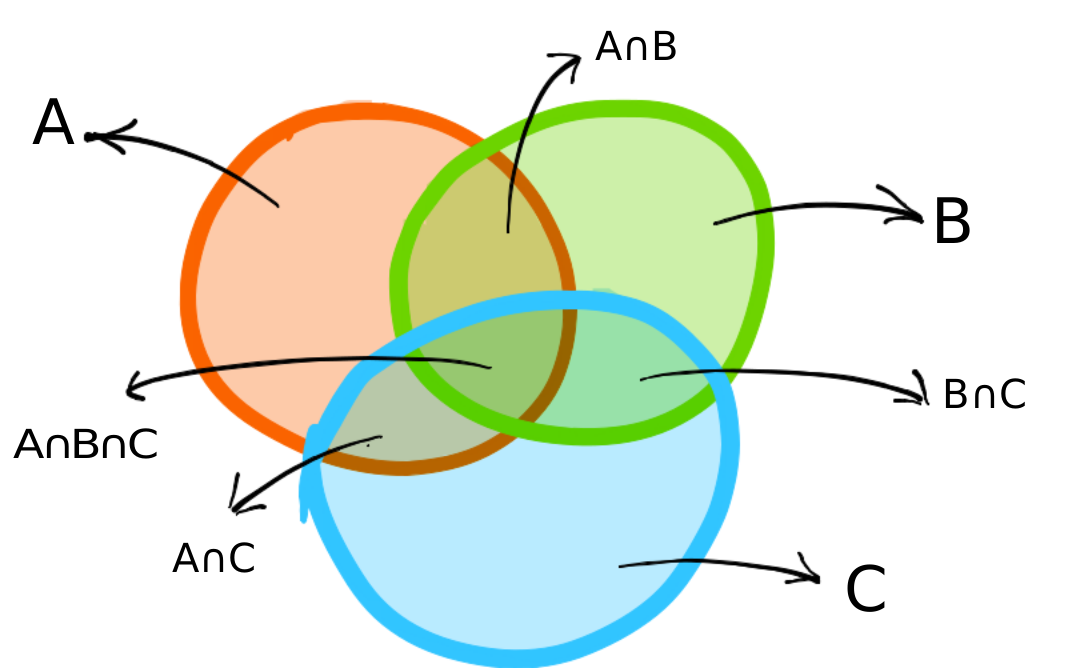
\includegraphics[scale=0.35]{FiguresBM/DV0.png}
    		\caption[Representación del diagrama de Venn para tres conjuntos]{Representación del diagrama de Venn para tres conjuntos. El círculo naranjo representa el conjunto $A$, el círculo verde representa el conjunto $B$ y el circulo celeste representa el conjunto $C$. Las secciones que se superponen dos círculos muestran la intersección de dos conjuntos y la superposición central es la intersección de los tres conjuntos.}
	\end{figure}
\end{center}

\subsection{Diferencia de conjuntos}
La diferencia entre dos conjuntos $A$ y $B$ es el conjunto de los elementos que pertenecen a $A$ y no pertenecen a $B$. La diferencia entre $A$ y $B$ se denota como $A-B$ o $A|B$. Escrito con cuantificadores queda de la siguiente manera: \\

\begin{equation}
A-B =\{x\in\mathcal{U}:x\in A\wedge x\notin B\}=\{x|x\in A\wedge x\notin B\}
\label{dif0}
\end{equation}
\begin{myexample}
Dado dos conjuntos finitos $A=\{a,b,c,d,e,f\}$ y $B=\{c,d,e,f,g,h\}$ determinar la diferencia $A-B$
\end{myexample}
Como se vio en la definición el conjunto resultante son los elementos que están en el conjunto $A$ pero no están en el conjunto $B$
\begin{equation*}
A-B=\{a,b\}
\end{equation*}

\begin{center}
	\begin{figure}[ht!]
	\centering
    		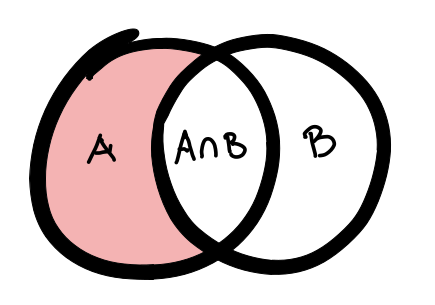
\includegraphics[scale=0.35]{FiguresBM/diferenciac.png}
    		\caption[Representación de diferencia de dos conjuntos]{Representación de diferencia de dos conjuntos usando el diagrama de Venn. Zona marcada con rojo marca $A-B$.}
	\end{figure}
\end{center}

se sacan los elementos que puedan estar en la intersección de ambos conjuntos y exclusivamente en el conjunto B.

\subsection{Complemento de un conjunto}
Dado el conjunto $A$, $\mathcal{U}-A$ se llama complemento de $A$ con respecto a $\mathcal{U}$ y se denota como $A^{c}$, $A'$ o $-A$. Entonces, en términos de cuantificadores lógicos el complemento se escribe de la siguiente manera:
\begin{equation}
A^{c}=\{x\in\mathcal{U}:x\notin A\}
\end{equation}
De la definición anterior se verifica que $\forall x\in\mathcal{U}$  una y solo una de la siguientes proposiciones:
\begin{equation*}
i)\hspace{2px} x\in A \hspace{20px} ii)\hspace{2px} x\in A^{c}
\end{equation*}

\begin{center}
	\begin{figure}[ht!]
	\centering
    		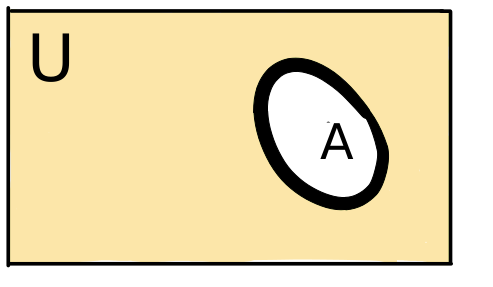
\includegraphics[scale=0.38]{FiguresBM/complemento.png}
    		\caption[Representación del complemento del conjunto $A$]{Representación del complemento del conjunto $A$. La zona oscurecida muestra el conjunto complemento, donde $\mathcal{U}$ es el conjunto universal.}
	\end{figure}
\end{center}

\subsection{Intersección de conjuntos }
La intersección de dos conjuntos $A$ y $B$ es el conjunto formado por todos los elementos comunes de los dos conjuntos. Se denota con el símbolo $A\cap B$ y se lee ``$A$ intersección $B$.\\
La intersección en términos de cuantificadores se escribe de la siguiente manera:\\
\begin{equation}
A\cap B=\{x\in\mathcal{U}:x\in A\wedge x\in B\}=\{x|x\in A\wedge x\in B\}
\end{equation} 

\begin{myexample}
Dado dos conjuntos finitos $A=\{a,b,c,d,e,f\}$ y $B=\{c,d,e,f,g,h\}$, determinar la intersección $A\cap B$
\end{myexample}
\begin{equation*}
A\cap B=\{c,d,e,f\}
\end{equation*}
\begin{myexample}
Dado dos conjuntos finitos $A=\{1,1,1,1,1,2\}$ y $B=\{1,2\}$, determinar la intersección $A\cap B$
\end{myexample}
\begin{equation*}
A\cap B=\{1,2\}
\end{equation*}

\begin{center}
	\begin{figure}[ht!]
	\centering
    		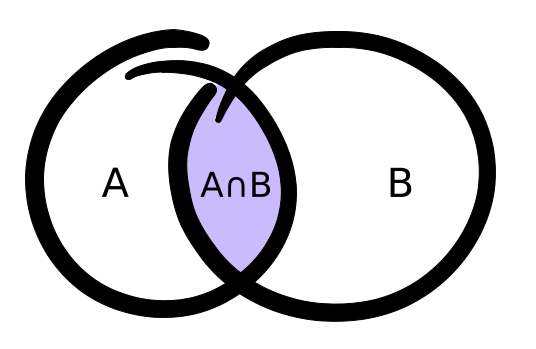
\includegraphics[scale=0.35]{FiguresBM/interseccion.png}
    		\caption[Representación de la intersección de dos conjuntos]{Representación de la intersección de dos conjuntos usando el diagrama de Venn. La zona oscurecida representa la intersección entre los conjuntos $A$ y $B$.}
	\end{figure}
\end{center}
Si dos conjuntos tienen intersección vacía se llaman \textit{conjuntos disjuntos}. Se escriben de la forma $A\cap B=\{\}$ o $A\cap B=\varnothing$.
\subsection{Unión de conjuntos}
La unión de dos conjuntos $A$ y $B$ contiene todos los elementos que pertenecen a $A$ y $B$. Esta operación es denotada por $A\cup B$ y se lee ``$A$ unido $B$'' o ``$A$ unión $B$''.\\
En términos de cuantificadores lógicos, la unión de conjuntos se representa de la siguiente manera:
\begin{equation}
A\cup B=\{x\in\mathcal{U}:x\in A\vee x\in B\}=\{x|x\in A\vee x\in B\}
\end{equation}
\begin{myexample}
Dado dos conjuntos finitos $A=\{a,b,c,d,e,f\}$ y $B=\{c,d,e,f,g,h\}$, determinar la unión $A\cup B$
\end{myexample}
\begin{equation*}
A\cup B=\{a,b,c,d,e,f,g,h\}
\end{equation*}
\begin{myexample}
Dado dos conjuntos finitos $A=\{1,1,1,1,1,1,2\}$ y $B=\{2,3\}$, determinar la unión $A\cup B$
\end{myexample}
\begin{equation*}
A\cup B=\{1,2,3\}
\end{equation*}

\begin{center}
	\begin{figure}[ht!]
	\centering
    		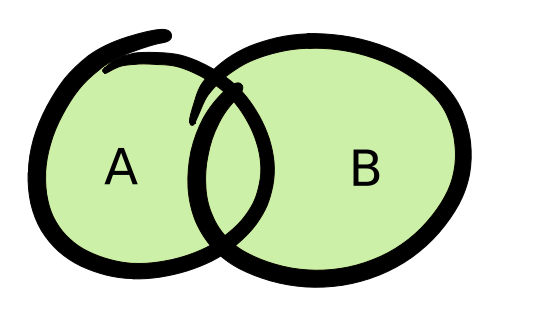
\includegraphics[scale=0.4]{FiguresBM/union.png}
    		\caption[Representación de la unión de dos conjuntos]{Representación de la unión de dos conjuntos usando el diagrama de Venn. La zona oscurecida muestra la unión entre el conjunto $A$ y $B$.}
	\end{figure}
\end{center}

\subsection{Diferencia simétrica de conjuntos}
La diferencia simétrica de dos conjuntos $A$ y $B$ es el conjunto que contiene la unión de ambos conjuntos, pero no considera la intersección de estos. La operación de diferencia simétrica se denota por $A\bigtriangleup B$ y en términos de cuantificadores se escribe de la siguiente manera:
\begin{equation*}
A\bigtriangleup B=\{x|x\in A\veebar B\}
\end{equation*}

\begin{center}
	\begin{figure}[ht!]
	\centering
    		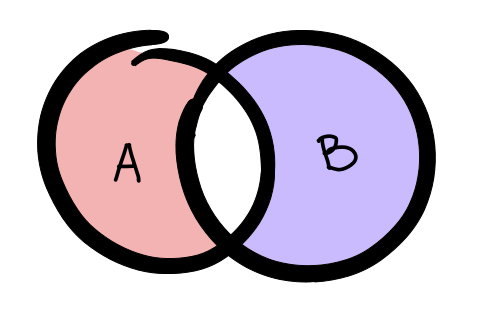
\includegraphics[scale=0.42]{FiguresBM/diferencias.png}
    		\caption[Representación de la diferencia simétrica entre el conjunto $A$ y $B$ ]{Representación de la diferencia simétrica entre el conjunto $A$ y $B$ usando el diagrama de Venn.}
	\end{figure}
\end{center}

\begin{myexample}
Sea dos conjuntos finitos $A=\{a,e,i,o,u\}$ y $B=\{a,b,c,d,e\}$. Calcular la diferencia simétrica entre los conjuntos $A$ y $B$.
\end{myexample}
\begin{eqnarray*}
A\bigtriangleup B =\{i,o,u,b,c,d\}
\end{eqnarray*}

\section{Propiedades de los conjuntos}
Con las operaciones vistas en (\ref{opc}) se ven importantes propiedades y ahora ocuparlas para reducir expresiones de dos o más conjuntos.

\subsection{Idempotencia}
La idempotencia es la propiedad de realizar una acción n-veces y aun así obtener el resultado como si se hubiera aplicado solo una vez.\\
\begin{eqnarray}
A\cup A&=& A\\
A\cap A&=& A
\end{eqnarray}

\begin{myexample}
Sea el conjunto finito $A=\{5,2,10\}$. Calcular $A\cup A$: 
\end{myexample}
\begin{eqnarray*}
A\cup A&=& \{5,2,10\}\cup\{5,2,10\} \nonumber\\
&=&\{5,2,10\} \\
&=&A
\end{eqnarray*}

%\begin{myexample}
%
%\end{myexample}
%\begin{eqnarray*}
%
%\end{eqnarray*}

\subsection{Conmutatividad}
La conmutatividad es la propiedad que tienen algunas operaciones en que el resultado de operar dos elementos no depende el orden en que se tomen estos mismos.\\
\begin{eqnarray}
A\cup B&=&B\cup A\\
A\cap B&=&B\cap A
\end{eqnarray}

\begin{myexample}
Sean los conjuntos finitos $A=\{Ibuprofeno,Naproxeno\}$ y \\ $B=\{ Aspirina,$ $Naproxeno,$ $Omeprazol \}$. Comprobar la propiedad conmutativa.
\end{myexample}
\begin{eqnarray*}
A\cap B&=& \{Ibuprofeno,Naproxeno\}\cap\{Aspirina,Naproxeno, Omeprazol \}\nonumber\\
&=& \{ Naproxeno\} \nonumber
\end{eqnarray*}
Análogamente
\begin{eqnarray*}
B\cap A&=&\{Aspirina, Naproxeno, Omeprazol \}\cap\{Ibuprofeno, Naproxeno\}\nonumber\\
&=& \{Naproxeno\}\nonumber\\
A\cap B &=& B\cap A \nonumber
\end{eqnarray*}

\subsection{Asociatividad}
La asociatividad es la propiedad de que el orden en que se ejecuten las operaciones no altera el resultado, siempre y cuando se mantenga intacto el orden de los elementos que se le aplica la operación (operandos).
\begin{eqnarray}
A\cup (B\cup C)&=&(A\cup B)\cup C\\
A\cap (B\cap C)&=&(A\cap B)\cap C
\end{eqnarray}
\subsection{Distributividad}
\begin{eqnarray}
A\cup (B\cap C)&=& (A\cup B)\cap(A\cup C)\label{distr0}\\
A\cap (B\cup C)&=& (A\cap B)\cup(A\cap C)
\end{eqnarray}

\begin{myexample}
Sean los conjuntos finitos $A=\{-5,-4,-3,-2,-1\}$, $B=\{-3,-2,-1,0,1,2,3\}$ y $C=\{-5,-2,-1,3,4\}$. Comprobar la propiedad distributiva
\end{myexample}
Primero se calcula el lado izquierdo de la ecuación (\ref{distr0}).
\begin{eqnarray}
A\cup (B\cap C) &=& \{-5,-4,-3,-2,-1\}\cup(\{-3,-2,-1,0,1,2,3\}\cap\{-5,-2,-1,3,4\}) \nonumber\\
&=& \{-5,-4,-3,-2,-1\}\cup\{-2,-1,3\}\nonumber\\
&=&\{-5,-4,-3,-2,-1,3\}\label{distr1}
\end{eqnarray}
ahora se desarrolla el lado derecho de la ecuación (\ref{distr0}).
\begin{eqnarray}
(A\cup B)\cap(A\cup C)&=&(\{-5,-4,-3,-2,-1,0,1,2,3\})\cap(\{-5,-4,-3,-2,-1,3,4\})\nonumber\\
&=&\{-5,-4,-3,-2,-1,3\}\label{distr2}
\end{eqnarray}
Como se puede ver, por las ecuaciones (\ref{distr1}) y (\ref{distr2}) se comprueba la propiedad distributiva de los conjuntos.

\subsection{Leyes de Morgan}
\begin{eqnarray}
(A\cup B)^{c}&=& A^{c}\cap B^{c}\\
(A\cap B)^{c}&=& A^{c}\cup B^{c}
\end{eqnarray}
\begin{myexample}
Demostrar mediante cuantificadores lógicos la expresión $(A\cap B)^{c}=A^{c}\cup B^{c}$
\end{myexample}

\begin{eqnarray}
x\in (A\cap B)^{c} &\Leftrightarrow & x\notin A\cap B \nonumber\\
&\Leftrightarrow & \sim ((x\in A)\wedge(x\in B))\nonumber\\
&\Leftrightarrow &\sim (x\in A)\vee\sim(x\in B)\nonumber\\
&\Leftrightarrow & x\in A^{c} \vee x\in B^{c}\nonumber\\
&\Leftrightarrow & x\in A^{c}\cup B^{c}\nonumber
\end{eqnarray}
Entonces se comprueba que $(A\cap B)^{c}=A^{c}\cup B^{c}$.


\section{Técnicas de conteo}
Para completar el conocimiento que se puede tener sobre un conjunto (o varios conjuntos) falta agregar las herramientas que nos permitan saber cuantos elementos tienen cada conjunto. Las técnicas de conteo solucionan esta problemática usando el concepto de cardinalidad (definido en \ref{cardinalidad}) y para dos casos, cuando los conjuntos no tienen intersección o si la tienen.
\subsection{Conteo en conjuntos disjuntos}
Como en este caso la intersección entre los conjuntos es vacía, la cardinalidad de la unión entre los conjuntos $A$ y $B$ está dada por:
\begin{equation}
|A\cup B|=|A|+|B| \label{conteo0}
\end{equation}
\begin{myexample}
Sea $A=\{1,2,3\}$ y $B=\{a,b,c\}$ dos conjuntos finitos y disjuntos. Mostrar la cardinalidad de la unión entre $A$ y $B$.
\end{myexample}
\begin{eqnarray*}
|A\cup B|=|A|+|B|=3+3=6
\end{eqnarray*}
Notar que $A\cup B=\{1,2,3,a,b,c\}$ y tiene cardinalidad 6. 
\begin{myexample}
En el examen único nacional de medicina (EUNACOM) del 2017\footnote{Informe final EUNACOM, enero 2018. Fuente: www.eunacom.cl} el área de Medicina interna tuvo $67$ preguntas, mientras que en pediatría fueron $29$. Si consideramos ambas áreas como conjuntos, ¿Cuál es la cardinalidad de la unión de ambos conjuntos? 
\end{myexample}
Identificaremos el conjunto de medicina interna como $MI$ y el de pediatría como $P$, ahora se aplica la ecuación (\ref{conteo0}) y resulta lo siguiente:
\begin{eqnarray}
|MI\cup P|=|MI|+|P|=67+29=96.
\end{eqnarray}

Además, mencionar que esto se puede expandir para $n$ conjuntos donde se debe sumar la cardinalidad de cada conjunto, ya que no hay intersección entre ellos.

\subsection{Conteo en conjuntos no disjuntos}
Para el caso en que si hay intersección entre dos conjuntos se sigue la misma lógica, pero se debe quitar la cardinalidad de la intersección para no cometer el error de contar dos veces algunos elementos.
\begin{equation}
|A\cup B|=|A|+|B|-|A\cap B|
\end{equation}
\begin{myexample}
Sea $A=\{1,2,3\}$ y $B=\{3,4,5\}$ dos conjuntos finitos y no disjuntos. Mostrar la cardinalidad de la unión entre estos dos conjuntos.
\end{myexample}
\begin{eqnarray}
|A\cup B|&=&|A|+|B|-|A\cap B|\nonumber\\
&=& 3+3-1=5\nonumber
\end{eqnarray}

\subsection{Conteo para la unión de tres conjuntos}
La ecuación para el caso de tres conjuntos se puede derivar de la ecuación para dos conjuntos no disjuntos.
\begin{eqnarray}
|A\cup B\cup C|&=&|A\cup (B\cup C)|\nonumber\\
&=&|A|+|B\cup C|-|A\cap (B\cup C)| \nonumber\\
&=&|A|+|B|+|C|-|B\cap C|-|A\cap (B\cup C)|\nonumber\\
&=&|A|+|B|+|C|-|B\cap C|-|(A\cap B)\cup(A\cap C)|\nonumber\\
&=&|A|+|B|+|C|-|B\cap C|-(|A\cap B|+|A\cap C|-|(A\cap B)\cap(A\cap C)|)\nonumber\\
&=&|A|+|B|+|C|-|B\cap C|-|A\cap B|-|A\cap C|+|(A\cap B)\cap(A\cap C)|\nonumber\\
&=&|A|+|B|+|C|-|B\cap C|-|A\cap B|-|A\cap C|+|A\cap B\cap C|
\label{uni3c}
\end{eqnarray}
La ecuación (\ref{uni3c}) muestra la ecuación para contar la unión de tres conjuntos no disjuntos.

Adicionalmente, desde el diagrama de Venn se puede definir las formulas para el número de elementos que solo se encuentran en un solo conjunto como solo en las intersecciones.\\

\begin{center}
\textbf{Número de elementos en un solo conjunto}\\
\end{center}


\noindent Los elementos que solo están en A:
\begin{eqnarray}
E_{A}=|A|-|A\cap B|-|A\cap C|+|A\cap B\cap C|
\end{eqnarray}
\noindent Los elementos que solo están en B:
\begin{eqnarray}
E_{B}=|B|-|A\cap B|-|B\cap C|+|A\cap B\cap C|
\end{eqnarray}
\noindent Los elementos que solo están en C:
\begin{eqnarray}
E_{C}=|C|-|A\cap C|-|B\cap C|+|A\cap B\cap C|
\end{eqnarray}

\begin{center}
\textbf{Número de elementos en la intersección de dos conjuntos, pero no en el tercero}\\
\end{center}

\noindent El número de elementos que están en $A\cap B$, pero no en C:\\
\begin{eqnarray}
E_{A\cap B}=|A\cap B|-|A\cap B\cap C|
\end{eqnarray}

\noindent El número de elementos que están en $A\cap C$, pero no en B:\\
\begin{eqnarray}
E_{A\cap C}=|A\cap C|-|A\cap B\cap C|
\end{eqnarray}

\noindent El número de elementos que están en $B\cap C$, pero no en A:\\
\begin{eqnarray}
E_{B\cap C}=|B\cap C|-|A\cap B\cap C|
\end{eqnarray}

\begin{center}
\textbf{Número de elementos en la unión de dos conjuntos, pero no en el tercero}\\
\end{center}

\noindent El número de elementos que está en $A$ o en $B$, pero no está en C:\\
\begin{eqnarray}
E_{A\cup B}=|A\cup B|-|A\cap B|-|B\cap C|+|A\cup B\cup C|
\end{eqnarray}

\noindent El número de elementos que está en $A$ o en $C$, pero no está en B:\\
\begin{eqnarray}
E_{A\cup C}=|A\cup C|-|A\cap B|-|B\cap C|+|A\cup B\cup C|
\end{eqnarray}

\noindent El número de elementos que está en $B$ o en $C$, pero no está en A:\\
\begin{eqnarray}
E_{B\cup C}=|B\cup C|-|A\cap B|-|A\cap C|+|A\cup B\cup C|
\end{eqnarray}

\begin{myexample}
Se encuestó a $100$ médicos sobre sus preferencias de especialidad y las respuestas arrojaron lo siguiente:
\end{myexample}
\begin{itemize}
	\item 32 Cirugía Pediátrica, $|CP|=32$.
	\item 20 Genética Clínica, $|GC|=20$.
	\item 45 Dermatología, $|D|=45$.
	\item 15 Cirugía pediátrica y Dermatología, $|CP\cap D|=15$.
	\item 7 Cirugía Pediátrica y Genética Clínica, $|CP\cap GC|=7$.
	\item 10 Genética Clínica y Dermatología, $|GC\cap D|=10$.
	\item 30 no prefieren ninguna de las tres especialidades.
\end{itemize}
\noindent a) Encontrar, el número de médicos que estudian las tres asignaturas.\\

Primero, notar que el número de médicos encuestados es el conjunto universo, entonces $\mathcal{U}=100$. Por lo que la unión de los tres conjuntos es:\\
\begin{eqnarray*}
|CP\cup GC\cup D|=100-30=70
\end{eqnarray*}
Segundo, de la ecuación (\ref{uni3c}) nos faltan dos términos, $|A\cup B\cup C|$ y $|A\cap B\cap C|$. Siendo el segundo el que se busca.

\begin{eqnarray*}
|CP\cup GC\cup D|&=&|CP|+|GC|+|D|-|CP\cap GC|-|CP\cap D|-|GC\cap D|+|CP\cap GC\cap D| \\
70&=&32+20+45-7-15-10+|CP\cap GC\cap D|\\
|CP\cap GC\cap D|&=&70-32-20-45+7+15+10\\
|CP\cap GC\cap D|&=&5\\
\end{eqnarray*}
Solo 5 médicos prefieren las tres especialidades.\\

\noindent  b) Encontrar el numero de médicos que prefieren una y solo una de las tres especialidades.\\

Se debe encontrar el número de médicos que prefiere una y solo una especialidad por separado.\\

\noindent Solo prefieren Cirugía Pediátrica:
\begin{eqnarray*}
|CP|-|CP\cap GC|-|CP\cap D|+|CP\cap GC\cap D| &=& 32-7-15+5=15\\
\end{eqnarray*}
Solo prefieren Genética Clínica:
\begin{eqnarray*}
|GC|-|GC\cap CP|-|GC\cap D|+|CP\cap GC\cap D| &=&20-7-10+5=8\\
\end{eqnarray*}
Dermatología :
\begin{eqnarray*}
|D|-|D\cap GC|-|D\cap CP|+|CP\cap GC\cap D| &=&45-10-15+5=25\\
\end{eqnarray*}
Finalmente el total de médicos que prefieren una y solo especialidad es: $15+8+25=48$ médicos.\\
	\lhead[\thepage]{CAPÍTULO \thechapter. \rightmark}
\rhead[CAPÍTULO \thechapter. \leftmark]{\thepage}
%======================================================================
\chapter{Números reales}
\label{nr}
\markboth{Números reales}{Números reales}
%======================================================================

%----------------------------------------------------------------------

%----------------------------------------------------------------------
En el capítulo (\ref{TC}) se vieron conjuntos de elementos que cuando tiene una característica en común se les llama conjuntos. Más explícitamente en el ejemplo (\ref{ejemplosNR}) se revisó los diferentes conjuntos de números que existen (No son los únicos). En el presente capítulo nos enfocaremos en el conjunto de los números reales, denotado por la letra $\mathbb{R}$.\\
Para representar los números reales, recurriremos al conjunto de los números irracionales ($\mathbb{I}$) y el conjunto de los números racionales ($\mathbb{Q}$), entonces la unión de estos dos conjuntos forman el conjunto de los números reales
\begin{eqnarray*}
\mathbb{R}&=&\mathbb{I}\cup \mathbb{Q} \nonumber\\
\mathbb{N}&\subset & \mathbb{Z }\subset \mathbb{Q}\subset \mathbb{R}\nonumber
\end{eqnarray*}
Mencionar que el conjunto de los números reales no es el más grande. El conjunto de los números complejos (denotado por la letra $\mathbb{C}$) es aún más grande y no se representa con una recta como reales sino con un plano de dos ejes.\\ 
\begin{figure}
	\centering
	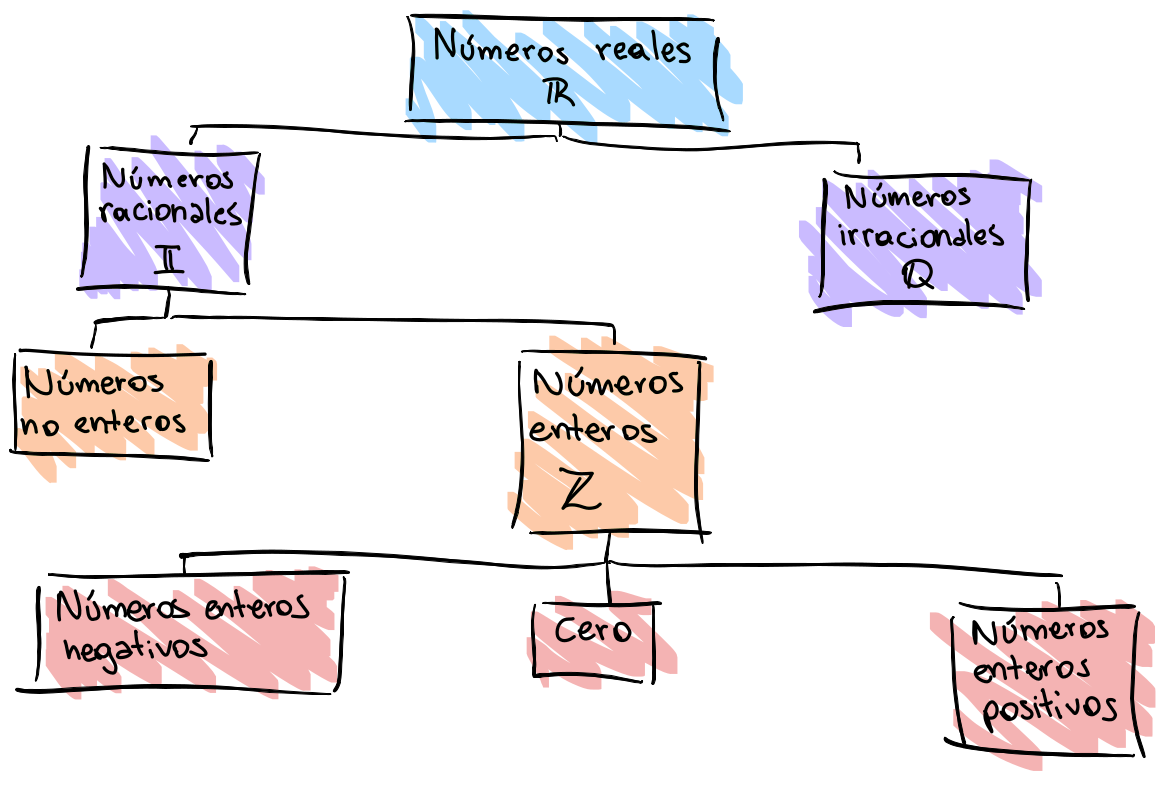
\includegraphics[scale=0.35]{esquemam.png}
	\caption[Esquema de los números reales]{Esquema de los números reales con los subconjuntos que lo conforman. }
\end{figure}
\begin{figure}
	\centering
	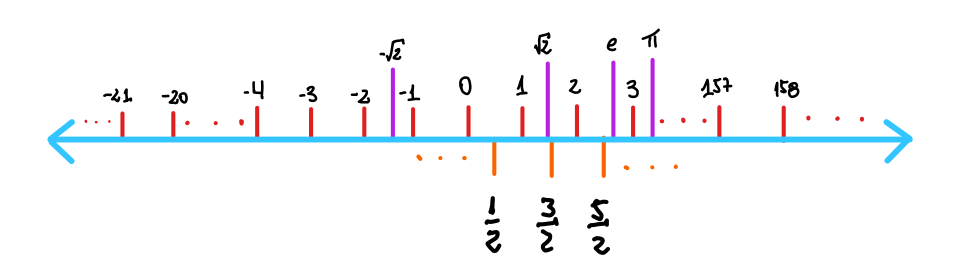
\includegraphics[scale=0.4]{rectar.png}
	\caption[Representación de la recta de los números reales]{Representación de la recta de los números reales mostrando algunos de los elementos pertenecientes a los subconjuntos que lo componen.}
	\label{rectar}
\end{figure}

\begin{myexample}
Representación de algunos elementos de los subconjuntos de los números reales
\end{myexample}

\begin{eqnarray}
\{1,3,100,263\}&\subset & \mathbb{N} \nonumber\\
\{-152,-5,0,7,670\}&\subset & \mathbb{Z} \nonumber\\
\left\{\dfrac{-3}{2},\dfrac{6}{2},\dfrac{25}{5},\dfrac{0}{9}\right\}&\subset & \mathbb{Q} \nonumber\\
\{e,\pi,\sqrt{2},\sqrt{7}\}&\subset & \mathbb{I} \nonumber\\
\left\{-10,\hspace{2px}0,\hspace{2px}\sqrt{6},\hspace{2px}2.333...,\hspace{2px}\pi,\hspace{2px}\dfrac{20}{7}\right\}&\subset & \mathbb{R} \nonumber
\end{eqnarray}

\section{Propiedades de los números reales}
\label{nr0}

El conjunto de los números reales contiene dos operaciones, una adición y una multiplicación que satisfacen las siguientes propiedades:
\subsection{Adición en los números reales}

\noindent 1) $a+(b+c)=(a+b)+c$, $\forall$ $a$, $b$, $c$ $\in \mathbb{R}$.\\

\noindent 2) $a+b=b+a$, $\forall$ $a,b\in \mathbb{R}$.\\

\noindent 3) Existe $0\in\mathbb{R}$ tal que $a+0=a$, $\forall a\in \mathbb{R}$.\\

\noindent 4) Para cada elemento $a \in \mathbb{R}$ existe un elemento $b\in\mathbb{R}$, tal que $a+b=0$. El elemento $b$ es el inverso aditivo del elemento $a$.\\

\begin{mydef}
\textbf{Sustracción.} $a-b=a+(-b)$, $\forall$ $a,b \in \mathbb{R}$ 
\end{mydef}


\subsection{Multiplicación en los números reales}
\noindent 1) $a\cdot(b\cdot c)=(a\cdot b)\cdot c$, $\forall a$, $b$, $c$ $\in \mathbb{R}$.\\

\noindent 2) $a\cdot b=b\cdot a$, $\forall$ $a$, $b$ $\in\mathbb{R}$.\\

\noindent 3) Existe $1\in\mathbb{R}$, $1\neq 0$, tal que $a\cdot 1=a$, $\forall a\in\mathbb{R}$.\\

\noindent 4) Para cada elemento $a\in\mathbb{R}$, no nulo, existe un elemento $c\in\mathbb{R}$, tal que $a\cdot c=1$. El elemento $c$ es el inverso multiplicativo de $a$ y todos los números lo tienen excepto el cero.\\

\begin{mydef}
\textbf{División.} $\dfrac{a}{b}=a\cdot b^{-1}$, $\forall a,b\in\mathbb{R}$, $b\neq 0$.
\end{mydef}

\subsection{Consecuencias de la adición y sustracción}
\label{consecu}
\noindent 1) Unicidad del 0 y del 1. Unicidad significa que existe solo un elemento dentro del conjunto, más específicamente, hay un solo elemento que cumple la acción del cero y el uno. \\

\noindent 2) Unicidad de los inversos. Tanto en la suma como en la multiplicación existe un solo inverso.\\

\noindent 3) $\forall a,b,c\in\mathbb{R}$, $a+c=b+c\Leftrightarrow a=b$. \\

\noindent 4) $\forall a,b,c\in\mathbb{R}$, $c\neq 0$, $a\cdot c=b\cdot c\Leftrightarrow a=b$. \\

\noindent 5) $a\cdot 0=0$, $\forall a\in\mathbb{R}$. \\

\noindent 6) $(-1)\cdot a=-a$, $\forall a\in\mathbb{R}$. \\

\noindent 7) $-(-a)=a$, $\forall a\in\mathbb{R}$. \\

\noindent 8) $(-a)\cdot b=a\cdot(-b)=-(a\cdot b)$; \hspace{8px} $(-a)\cdot(-b)=a\cdot b$, $\forall a,b\in\mathbb{R}$. \\

\noindent 9) Si $a\neq 0$, la ecuación $ax+b=c$ tiene solución única en $\mathbb{R}$. \\

\noindent 10) $-(a+b)=(-a)+(-b)=-a-b$, $\forall a,b\in\mathbb{R}$. \\

\noindent 11) $-(a+b)=-a-b,$ $-(-a-b)=a+b$, $\forall a,b\in\mathbb{R}$. \\

\noindent 12) $\forall a,b\in\mathbb{R}:$ $a\cdot b=0\Leftrightarrow a=0\vee b=0$. \\

\noindent 13) Si $a\neq 0$, entonces $(a^{-1})^{-1}=a$. \\

\noindent 14) Si $a,b\neq 0$, entonces $(a\cdot b)^{-1}=a^{-1}b^{-1}$. \\

\noindent 15) Si $b,d\neq 0$, $\dfrac{a}{b}=\dfrac{c}{d}\Leftrightarrow a\cdot d =b\cdot c$. \\

\noindent 16) Si $b,c\neq 0$, $\dfrac{a}{b}=\dfrac{a\cdot c}{b\cdot c}$. \\

\noindent 17) Si $c\neq 0$, $\dfrac{a}{c}\pm\dfrac{b}{c}=\dfrac{a\pm b}{c}$. \\

\noindent 18) Si $b,d \neq 0$, $\dfrac{a}{b}\cdot\dfrac{c}{d}=\dfrac{a\cdot c}{b\cdot d}$. \\

\noindent 19) Si $b,c,d\neq 0$, $\dfrac{a/b}{c/d}=\dfrac{a}{b}\cdot\dfrac{d}{c}$. \\

\noindent 20) Si $b,d\neq 0$, $\dfrac{a}{b}\pm\dfrac{c}{d}=\dfrac{a\cdot d\pm b\cdot c}{b\cdot d}$. \\
\section{Porcentajes}
De la figura (\ref{rectar}) se  pueden ver algunos elementos de los números reales son fracciones, que a su vez son números decimales. Mencionar que todo número real puede ser expresado como número decimal.
\begin{eqnarray*}
\dfrac{25}{7}=3.57142...
\end{eqnarray*}
Para algunos casos prácticos sirven estos decimales o fracciones para representar porcentajes de  alguna cantidad. Cuando se dice ``un $x$ porcentaje de algo'' se representa como
\begin{eqnarray}
\dfrac{x}{100}\cdot Cantidad
\end{eqnarray} 
Donde $x$ es el porcentaje que busco calcular de la cantidad. En algunos casos simplemente se multiplica la fracción y se multiplica directamente el número decimal por la cantidad

\begin{myexample}
Calcular el $20\%$ de $120$:
\begin{eqnarray*}
x_{20}&=&\dfrac{20}{100}\cdot 120\\
x_{20}&=&\dfrac{1}{5}\cdot 120\\
x_{20}&=&24
\end{eqnarray*}
\end{myexample}

Para otro caso que se utilizan los porcentajes, es para calcular el porcentaje de crecimiento o decrecimiento de cierta cantidad.\\

\noindent \textit{Porcentaje de aumento:}\\
\begin{eqnarray}
\dfrac{Cantidad\hspace{3px}de\hspace{3px}aumento}{Cantidad\hspace{3px}original}\times 100\%
\end{eqnarray}

\begin{eqnarray}
\dfrac{Valor\hspace{3px}final\hspace{3px}-\hspace{3px}Valor\hspace{3px}inicial}{Valor\hspace{3px}inicial}\times 100\%= \dfrac{V_{f}-V_{i}}{V_{i}}\times 100\%
\end{eqnarray}


\noindent \textit{Porcentaje de decrecimiento:}\\
\begin{eqnarray}
\dfrac{Cantidad\hspace{3px}de\hspace{3px}decrecimiento}{Cantidad\hspace{3px}original}\times 100\%
\end{eqnarray}

\begin{eqnarray}
\dfrac{Valor\hspace{3px}inicial\hspace{3px}-\hspace{3px}Valor\hspace{3px}final}{Valor\hspace{3px}inicial}\times 100\%=\dfrac{V_{i}-V_{f}}{V_{i}}\times 100\%
\label{percent1}
\end{eqnarray}


\noindent \textit{Porcentaje de transmición:}\\

\begin{eqnarray}
\dfrac{Cantidad\hspace{3px}despu\acute{e} s\hspace{3px}de\hspace{3px}Transmitirse}{Cantidad\hspace{3px}original}\times 100\%
\label{percent2}
\end{eqnarray}

\begin{myexample}
Un día por un canal entraron $150$ litros de agua, pero como estaba roto salieron solo $100$ litros, ¿Cuál es el porcentaje de transmisión del canal?\\

Sol: Primero, se identifica las cantidades que se deben reemplazar en (\ref{percent2}). 
\begin{eqnarray*}
\dfrac{100 \hspace{3px}litros}{150\hspace{3px}litros}&\times & 100\%\\
\dfrac{2}{3}&\times & 100\%\\
& 66,7\% &
\end{eqnarray*}
\end{myexample}

\begin{myexample}
El ejemplo anterior se puede resolver también con la formula de decreciemiento. Si definimos $V_{i}=150$ $litros$ y $V_{f}=100$ $litros$. 
\begin{eqnarray*}
\dfrac{V_{i}-V_{f}}{V_{i}}\times 100\% &=&\dfrac{150-100\hspace{3px}litros}{150\hspace{3px}litros}\times 100\%\\
&=& \dfrac{50\hspace{3px}litros}{150\hspace{3px}litros}\times 100\%\\
&=&\dfrac{1}{3}\times 100\%\\
&=&33,3\%
\end{eqnarray*}
\end{myexample}

Con las fórmulas de porcentaje se puede obtener diferente información desde un mismo problema según lo que uno necesite.\\
 
\section{Desigualdades}

En la figura (\ref{rectar}) se muestra la recta de los números reales, donde uno puede definir el elemento cero como el \textit{origen} y cada número, ya sea positivo o negativo, tener una distancia con respecto a ese origen. Cada número real puede representarte como un punto en esta recta que se llama \textit{coordenada}, pero usualmente solo se dice $5$ y no ``el punto $5$''.\\
Esta distancia que tienen los números permite dar un orden a los números reales, entonces si tomamos dos elementos $a$ y $b$ se puede decir las siguientes afirmaciones.\\

Si $a$ está a la izquierda de $b$, se dice que $a$ es menor que $b$ y se denota $a<b$. El otro caso es que si $a$ está a la derecha de $b$, entonces se dice que $a$ es mayor que $b$ y se denota $a>b$. Siguiendo esa lógica están los caso de menor o igual que se denota como $a\leq b$ y mayor igual $a\geq b$ que agrega la posibilidad que los elementos sean iguales. Estos cuatro elementos son los símbolos de las desigualdades.\\

Para definir las propiedades de las desigualdades se debe utilizar un subconjunto de los números reales que llamaremos $\mathbb{P}$ ($\mathbb{P}\subset\mathbb{R}$) donde sus elementos son los números positivos.\\

\noindent 1) $\forall a,b\in\mathbb{R}$, $a,b\in\mathbb{P}\Rightarrow a+b\in\mathbb{P}$ \\

\noindent 2) $\forall a,b\in\mathbb{R}$, $a,b\in\mathbb{P}\Rightarrow a\cdot b\in\mathbb{P}$ \\

\noindent Dado $a\in\mathbb{R}$, se verifica una y solo una de las alternativas:\\
\begin{eqnarray*}
a\in\mathbb{P}, \hspace{3px} a=0, \hspace{3px} -a\in\mathbb{R}
\end{eqnarray*}

\begin{mydef}
Dado $a,b\in\mathbb{R}$ se define:\\

\noindent 1) $a<b\Leftrightarrow b-a\in\mathbb{P}$.\\
\noindent 2) $a\leq b\Leftrightarrow a<b\vee a=b$. \\
\noindent 3) $a>b\Leftrightarrow b<a$. \\
\noindent 4) $a\geq b\Leftrightarrow b\leq a$. \\
\end{mydef}

\subsection{Propiedades de las desigualdades}

\noindent 1) $\forall a\in\mathbb{R}$, $a>0\Leftrightarrow a\in\mathbb{P}$ \\

\noindent 2) $a\in\mathbb{R}$,  $a<0\Leftrightarrow -a>0$ \\
\noindent 3) Para cada $a\neq 0$, $a^{2}>0$ \\
\noindent 4) Para $a,b,c\in\mathbb{R}$, 
$$\left\{\begin{array}{ll} 
a<b \\
\hspace{35px}\Rightarrow a<c\\
b<c
\end{array} \right. \\$$

\noindent 5) Para $a,b,c\in\mathbb{R}$ $a<b\Leftrightarrow a+c<b+c$\\

\noindent 6) Para $a,b,c,d\in\mathbb{R}$
$$
\left\{\begin{array}{ll}
a<b\\
\hspace{35px} \Rightarrow a+c<b+d\\
c<d
\end{array}\right. $$\\

\noindent 7) $a,b,c\in\mathbb{R}, c>0$, $a<b\Leftrightarrow a\cdot c< b\cdot c$\\

\noindent 8) $a,b,c\in\mathbb{R}, c<0$, $a<b\Leftrightarrow a\cdot c> b\cdot c$\\

\noindent 9) $a>0\Leftrightarrow a^{-1}>0$, \hspace{10px} $a<0\Leftrightarrow a^{-1}<0$

\noindent 10) $$ a\cdot b>0\Leftrightarrow \left\{ 
\begin{array}{ll}
a>0 \wedge b>0\\
\vee \\
a<0 \wedge b<0
\end{array}
\right. $$

\noindent 11) $$ a\cdot b<0 \left\{\begin{array}{ll}
a>0 \wedge b<0\\
\vee \\
a<0 \wedge b>0
\end{array} \right.$$

\noindent 12) Para $a,b>0$, $a<b\Leftrightarrow a^{-1}>b^{-1}$

\subsection{Intervalos con desigualdades}
Es momento de juntar lo visto hasta el momento de conjuntos con los conceptos de las desigualdades. Utilizaremos el paréntesis cuadrado (en algunos textos ocupan otros tipos de paréntesis) para identificar cuando un intervalo es \textit{cerrado} o \textit{abierto}.\\
\begin{eqnarray}
\left] a,b\right[ =\left\{x\in\mathbb{R}:a<x<b\right\} \label{abierto}\\
\left[ a,b\right] = \left\{x\in\mathbb{R}:a\leq x\leq b\right\}\label{cerrado} \\
\left[a,b\right[=\left\{x\in\mathbb{R}:a\leq x< b\right\}\label{abiertob} \\
\left]a,b\right]=\left\{x\in\mathbb{R}:a< x\leq b\right\} \label{abiertoa}
\end{eqnarray}
El caso (\ref{abierto}) se llama un intervalo abierto en ambos extremos o solamente abierto, esto significa que los elementos $a$ y $b$ no pertenecen al conjunto. Para el caso (\ref{cerrado}) es un conjunto cerrado, por lo que si considera a los elementos $a$ y $b$. Los casos (\ref{abiertob}) y (\ref{abiertoa}) son abiertos en un solo extremo y siguen las mismas reglas que los otros dos casos anteriores. Cuando hay un infinito en el intervalo siempre se considera abierto por ese extremo.
\begin{eqnarray}
\left]a,+\infty\right[=\{x\in\mathbb{R}:x>a\}\\
\left[a,+\infty\right[=\{x\in\mathbb{R}:x\geq a\}\\
\left]-\infty ,a\right[=\{x\in\mathbb{R}:x< a\}\\
\left]-\infty ,a\right]=\{x\in\mathbb{R}:x\leq a\}
\label{interif}
\end{eqnarray}

\section{Valor absoluto}
Así como anteriormente se mencionó que la recta permite dar orden a los números reales, también puede representar una distancia. Esta distancia que tiene un elemento dado con respecto al origen es el \textit{valor absoluto}. Como no hay distancias negativas, la distancia es la misma para un elemento $a$ como para un elemento $-a$. La notación son dos barras verticales $||$.

\begin{mydef}
\textbf{Valor absoluto}. Sea $a\in\mathbb{R}$, entonces el valor absoluto de un número se define como:\

$$ |a| \left\{\begin{array}{ll}
a, & si \hspace{6px} a\geq 0\\
-a, & si \hspace{6px} a<0 
\end{array} \hspace{6px} \right.$$
\label{absdef}
\end{mydef}

\subsection{Propiedades del valor absoluto}
\label{Propabs}
\noindent 1) $|a|\geq 0$, $\forall a\in\mathbb{R}$ \\

\noindent 2) $\forall a\in\mathbb{R}$, $|a|=0\Leftrightarrow a=0$ \\

\noindent 3) $\forall a\in\mathbb{R}$, $|-a|=|a|$ \\

\noindent 4) $\forall a,b\in\mathbb{R}$, $|a\cdot b|=|a|\cdot|b|$ \\

\noindent 5) $\forall a,b\in\mathbb{R}$, $b\neq 0$, $\left|\dfrac{a}{b}\right|=\dfrac{|a|}{|b|}$ \\

\noindent 6) $\forall a,b\in\mathbb{R}$, $|a \pm b|\leq |a|+|b|$ \\

\noindent 7) $\forall a,b\in\mathbb{R}$, $||a|-|b||\leq |a\pm b|$ \\

\noindent 8) $\forall a,b\in\mathbb{R}$, $|a|=|b|\Rightarrow a=b \vee a= -b$ \\

\noindent 9) Si $c>0$, entonces $\forall x\in\mathbb{R}$ se cumple que:\\

9.1) $|x|=c\Leftrightarrow x=c \vee x=-c$ \\

9.2) $|x|<c\Leftrightarrow -c<x<c \Leftrightarrow -c<x\wedge x<c$\\

9.3) $|x|>c\Leftrightarrow x>c \vee x<-c$
\begin{center}
	\begin{figure}[h!]
		\centering
		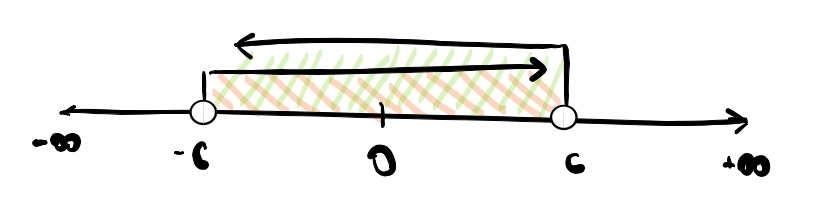
\includegraphics[scale=0.55]{abs0.png}
		\caption[Representación de un caso de valor absoluto de la propiedad 9.2]{Representación de un caso de valor absoluto de la propiedad 9.2. La zona sombreada es donde se encuentre la variable $x$ y las flechas muestran el sentido de la desigualdad particular. El resultado es la intersección de ambas condiciones.}
	\end{figure}
\end{center}
\begin{center}
	\begin{figure}[h!]
		\centering
		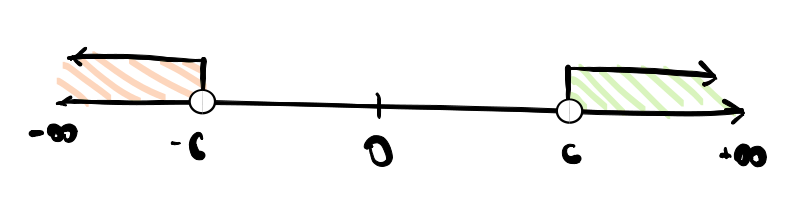
\includegraphics[scale=0.5]{abs1.png}
		\caption[Representación de un caso de valor absoluto de la propiedad 9.3]{Representación de un caso de valor absoluto de la propiedad 9.3. La zona sombreada es donde se encuentre la variable $x$ y las flechas muestran el sentido de la desigualdad particular. El resultado es la unión de ambas condiciones.}
	\end{figure}
\end{center}

\begin{myexample}
Ejercicios de valor absoluto.
\end{myexample}
\begin{eqnarray*}
&a)& |2|=2\\
&b)&|-2|=2\\
&c)&|5-7|=|-2|=2\\
&d)&|-3|-|-10|=3-(10)=-7
\end{eqnarray*}

\begin{myexample}
Encontrar el signo de la expresión $|x-6|$ para los casos cuando $a)$ $x>6$, $b)$ $x=6$ y $c)$ $x<6$
\end{myexample}
\noindent a) Primero notar que la variable toma cualquier valor mayor a $6$ y no considera al mismo número $6$. Se puede tomar cualquier número del conjunto para ver el signo del valor absoluto, por ejemplo el número $10$.\\
\begin{eqnarray}
|x-6|=|10-6|=|4|=4 \label{vaplus}
\end{eqnarray}
Entonces, de la ecuación (\ref{vaplus}) se concluye que el valor absoluto es positivo, en consecuencia $|x-6|=x-6$ para el caso cuando $x>6$.\\

\noindent b) Al igual que el caso anterior, se considera un caso particular cuando $x=6$.
\begin{eqnarray}
|x-6|=|6-6|=|0|=0
\end{eqnarray}

\noindent c) Para este último caso tomaremos un número de ejemplo, para ver el comportamiento del valor absoluto en este conjunto.
\begin{eqnarray}
|x-6|=|-10-6|=|-16|=16  \label{vapmenos}
\end{eqnarray} 
En la ecuación (\ref{vapmenos}) el resultado final es positivo por la operación del valor absoluto, pero $x-6$ es negativo por lo que se concluye que $|x-6|=-(x-6)=6-x$ cuando $x<6$.

\section{Exponentes}
\label{exponentes}
Cuando se suma varias veces una variable, para acortar la notación se escribe el número de las veces que se repite la variable y esto se multiplica por la variable, como por ejemplo $w+w+w+s+s=3w+2s$. Para el caso de la multiplicación de variables elevados a un número están las reglas de los exponentes (ya sean números enteros o fracciones) que veremos a continuación.\\

\begin{eqnarray}
x^{m}x^{n}&=&x^{m+n}\\
\left(\dfrac{x}{y}\right)^{n}&=&\dfrac{x^{n}}{y^{n}}\\
(x^{m})^{n}&=&x^{mn}\\
\dfrac{x^{m}}{x^{n}}&=&x^{m-n}\\
(xy)^{n}&=&x^{n}y^{n}
\end{eqnarray}

\subsection{Radicales}
Como se mencionó en la presentación del capítulo de exponentes, hay casos que los exponentes son fracciones y que se traducen en raíces (cuadradas, cúbicas, etc.) de la forma $\sqrt[n]{x}$, donde lo que está dentro de la raíz se llama radicando y $n$ es el índice de la raíz. Hay situaciones en que se llega a ecuaciones como $x^{2}=25$ o $y^{3}=64$ y las soluciones a estas ecuaciones se llaman \textit{raíces}, es decir, para este caso las raíces serían $5$ y el $4$ respectivamente. 
\begin{mydef}
Sea $x$ un número real y $n\geq 2$ es un número entero positivo.\\

\noindent i) Si $x>0$, entonces la raíz n-ésima principal de $\sqrt[n]{x}$  es el número r positivo tal que $x=r^{n}$.\\

\noindent ii) Si $x<0$ y n es un número entero positivo impar, entonces la raíz n-sima principal de $\sqrt[n]{x}$ es un número r negativo tal que $x=r^{n}$. Por ejemplo, la raíz cúbica está definida para cualquier número impar. \\

\noindent iii) Si $x<0$ y n es un número entero positivo par, entonces $\sqrt[n]{x}$ no es un número real. Pertenece a los números complejos ($x\in \mathbb{C}$). \\

\noindent iv) Si $x=0$, entonces $\sqrt[n]{x}=0$. \\
\end{mydef}

Las leyes que sirven para simplificar en los números radicales son las siguientes:\\
\begin{eqnarray}
&a)& (\sqrt[n]{x})^{n}=x \\
&b)& \sqrt[n]{xy}=\sqrt{x}\sqrt{y} \\
&c)& \sqrt[m]{\sqrt[n]{x}}=\sqrt[mn]{x}\\
&d)& \sqrt[n]{\dfrac{x}{y}}=\dfrac{\sqrt[n]{x}}{\sqrt[n]{y}}\\
&e)& \sqrt[n]{x^{n}}=\left\{\begin{array}{ll}
x&,\hspace{6px} si\hspace{2px} n\hspace{2px} es\hspace{2px} impar.\\
|x|& ,\hspace{6px} si\hspace{2px} n\hspace{2px} es\hspace{2px}par.
\end{array} \right.
\end{eqnarray}

\begin{myexample}
Ejercicios de exponentes
\end{myexample}
\begin{eqnarray*}
&a)& 77\cdot 77 \cdot 77\cdot 77 =77^{4}\\
&b)& 8^{-3}=\dfrac{1}{8^{3}}=\dfrac{1}{8\cdot 8\cdot 8}=\dfrac{1}{512}\\
&c)& \sqrt{2}=2^{1/2}\\
&d)& \sqrt[3]{10^{2}}=10^{2/3}\\
&e)& -5^{2}=-(5\cdot 5)=-25\\
&f)& (-5)^{2}=25\\
&g)& \sqrt{\dfrac{x^{2}}{25}}=\dfrac{\sqrt{x^{2}}}{\sqrt{25}}=\dfrac{|x|}{5}\\
&h)& \sqrt[3]{-8}=-2\\
&i)& \sqrt{256}=\sqrt{2^{8}}=2^{8/2}=2^{4}=16
\end{eqnarray*}

\subsection{Racionalización}
Se le llama racionalizar cuando ocupamos una operación matemática para quitar las raíces del numerador o denominador de una fracción. La técnica implica multiplicar por un \textit{uno} camuflado, por ejemplo:
\begin{equation*}
\dfrac{1+\sqrt{3}}{\sqrt{5}}=\dfrac{1+\sqrt{3}}{\sqrt{5}}\cdot\dfrac{\sqrt{5}}{\sqrt{5}}=\dfrac{(1+\sqrt{3})\sqrt{5}}{\sqrt{5}\cdot\sqrt{5}}=\dfrac{\sqrt{5}+\sqrt{15}}{\sqrt{5^{2}}}=\dfrac{\sqrt{5}+\sqrt{15}}{5}
\end{equation*}
Cuando el término es un factor de la forma $(\sqrt{x}\pm\sqrt{y})$ se debe multiplicar por el mismo término pero conjugado\footnote{El conjugado de una suma de números o variables consiste en cambiar el signo central entre ambos, osea que la expresión $a+b$ cambia a $a-b$, si se da el caso de $-a+b$ cambia a $-a-b$.}, es decir, el signo central es el opuesto.
$(\sqrt{x}\mp\sqrt{y})$.\\
\begin{eqnarray*}
(\sqrt{x}+\sqrt{y})(\sqrt{x}-\sqrt{y})&=& \sqrt{x}(\sqrt{x}-\sqrt{y})+\sqrt{y}(\sqrt{x}-\sqrt{y})\\
&=& (x-\sqrt{xy})+(\sqrt{yx}-y)\\
&=& x-y
\end{eqnarray*}

\begin{myexample}
Racionalizar la siguiente expresión fraccional
\end{myexample}
\begin{eqnarray*}
\dfrac{1}{\sqrt{x}+3}=\dfrac{1}{\sqrt{x}+3}\cdot \dfrac{\sqrt{x}-3}{\sqrt{x}-3}=\dfrac{\sqrt{x}-3}{x-9}
\end{eqnarray*}

Para el caso en que solo sea un término de raíz en la fracción, se debe multiplicar por el mismo termino.
\begin{eqnarray}
\dfrac{a}{\sqrt[n]{x^{k}}}\cdot\dfrac{\sqrt[n]{x^{n-k}}}{\sqrt[n]{x^{n-k}}}=\dfrac{a\sqrt[n]{x^{n-k}}}{\sqrt[n]{x^{k}}\sqrt[n]{x^{n-k}}}=\dfrac{a\sqrt[n]{x^{n-k}}}{\sqrt[n]{x^{k}\cdot x^{n-k}}}=\dfrac{a\sqrt[n]{x^{n-k}}}{\sqrt[n]{x^{k+n-k}}}=\dfrac{a\sqrt[n]{x^{n-k}}}{\sqrt[n]{x^{n}}}=\dfrac{a\sqrt[n]{x^{n-k}}}{x}
\end{eqnarray} 
Donde el número $k$ es al que está elevado el número dentro de la raíz y $n$ es la $n-$é$sima$ raíz del número.
\section{Factorización de polinomios}

\begin{mydef}
Un polinomio de grado $n$ en la variable $x$ es cualquier expresión algebraica de la forma:
\begin{eqnarray}
a_{n}x^{n}+a_{n-1}x^{n-1}+\cdots +a_{2}x^{2}+a_{1}x+a_{0}
\label{polg00}
\end{eqnarray}
con $a_{n}\neq 0$, $n$ es un número entero no negativo y $a_{i}$, $i=0,1,...,n$ son números reales.
\end{mydef}
Para los casos particulares, cuando $n=0$ es una constante, $n=1$ es un polinomio lineal, $n=2$ es un polinomio cuadratico, $n=3$ es un polinomio cúbico y para los $n\geq 4$ son polinomios de orden $n$.\\
\begin{myexample}
Sea  $5x^{4}+3x^{2}+1$ un polinomio de orden 4. Se identifican los términos desde la ecuación (\ref{polg00}) con el caso de $n=4$.
\begin{eqnarray*}
5x^{4}+3x^{2}+1&=& a_{4}x^{4}+a_{3}x^{3}+a_{2}x^{2}+a_{1}x+a_{0}x^{0}\\
&=& 5x^{4}+0x^{3}+3x^{2}+0x+1x^{0}\\
\end{eqnarray*}
Se deduce que $a_{4}=5$, $a_{3}=0$, $a_{2}=3$, $a_{1}=0$ y $a_{0}=1$.
\end{myexample}

Puede darse el caso en que hay una expresión que permite escribir un polinomio como producto de otro polinomio, esto se llama factorización. Es utilizado para simplificar resultados o separar ciertas variables. 

\begin{myexample}
Factorizar el siguiente polinomio.
\end{myexample}
\begin{eqnarray*}
6x^{4}y^{4}-4x^{2}y^{2}+10\sqrt{2}xy^{3}-2xy^{2}&=& 2xy^{2}(3x^{3}y^{2}-2x+5\sqrt{2}y-1)
\end{eqnarray*}
Lo importante en la factorización es encontrar el factor común que tienen los términos. Este factor puede ser común en todos los términos o solo en algunos.\\

\subsection{Factorización de polinomios cuadráticos}
\label{factor0}
En algunos casos es posible factorizar los polinomios cuadráticos de la forma $ax^{2}+bx+c$, donde los coeficientes $a$, $b$ y $c$ son números enteros, como 
\begin{eqnarray}
(Ax+B)(Cx+D) \label{fac0}
\end{eqnarray}
Donde $A$, $B$, $C$ y $D$ son también números enteros. Para comenzar solo consideraremos el caso en que $a=1$, entonces la ecuación queda de la forma $x^{2}+bx+c$ y los factores quedan definidos de la siguiente manera\\
\begin{eqnarray}
(x+B)(x+D) \label{fac1}
\end{eqnarray}
Si se expande la ecuación (\ref{fac1}):\\
\begin{eqnarray}
(x+B)(x+D)&=& x(x+D)+B(x+D)\nonumber\\
&=&x^{2}+xD+Bx+BD \nonumber\\
&=&x^{2}+x(D+B)+BD \label{expfac}
\end{eqnarray}
ahora se puede comparar la ecuación cuadrática término por término con la ecuación (\ref{expfac}). Se puede deducir las siguientes relaciones:
\begin{eqnarray*}
B+D=b \hspace{6px}y \hspace{6px}BD=c 
\end{eqnarray*}
\begin{myexample}
Factorizar el polinomio cuadrático de la forma $x^{2}-9x+18$
\end{myexample}
Los coeficientes son $b=-9$ y $c=18$, entonces $B+D=-9$ y $BD=18$. La segunda relación se puede escribir de diferentes formas:
\begin{eqnarray*}
1(18),\hspace{6px}2(9),\hspace{6px}3(6),\hspace{6px}-1(-18),\hspace{6px}-2(-9),\hspace{6px}o \hspace{6px}-3(-6),
\end{eqnarray*}
pero de todas las opciones anteriores solo sirve el caso en que  $B=-3$ y $D=-6$. Entonces los factores queda de la forma 
\begin{eqnarray*}
x^{2}-9x+18=(x-3)(x-6)
\end{eqnarray*}

\subsubsection{Polinomio cuadrática en caso general}
Para el caso  general donde el polinomio tiene la forma $ax^{2}+bx+c=0$ se debe aplicar la formula de ecuación cuadrática
\begin{eqnarray}
x_{\pm}=\dfrac{-b\pm\sqrt{b^{2}-4ac}}{2a}
\label{ecccuadra}
\end{eqnarray}
que se separa en dos soluciones, que son los números que componen los factores 
\begin{eqnarray}
x_{+}=\dfrac{-b+\sqrt{b^{2}-4ac}}{2a} \hspace{6px}y\hspace{6px}x_{-}=\dfrac{-b-\sqrt{b^{2}-4ac}}{2a}
\end{eqnarray}
Entonces los factores son:
\begin{eqnarray}
ax^{2}+bx+c&=&( x-x_{+})(x-x_{-})\\
&=&\left( x-\dfrac{-b+\sqrt{b^{2}-4ac}}{2a} \right) \left( x-\dfrac{-b-\sqrt{b^{2}-4ac}}{2a}\right)
\end{eqnarray}

\begin{myexample}
Resolver la ecuación cuadrática $5x^{2}+6x+1=0$
\end{myexample}
\begin{eqnarray*}
x&=&\dfrac{-6\pm\sqrt{6^{2}-4(5)(1)}}{2(5)}\\
&=&\dfrac{-6\pm\sqrt{36-20}}{10}\\
&=&\dfrac{-6\pm\sqrt{16}}{10}\\
&=&\dfrac{-6\pm 4}{10}\\
x_{+}=\dfrac{-6+ 4}{10} &y& x_{-}=\dfrac{-6- 4}{10}\\
x_{+}=\dfrac{-2}{10} &y& x_{-}=\dfrac{-10}{10}\\
x_{+}=\dfrac{-1}{5} &y& x_{-}=-1\\
\left(x+\dfrac{1}{5}\right)&\wedge &\left( x+1\right)=0
\end{eqnarray*}

Algo importante a notar en la ecuación (\ref{ecccuadra}) es el término que está bajo la raíz cuadrad al cual se le llama determinante. El término es $\sqrt{b^{2}-4ac}$ y se desprenden 3 casos posibles

\begin{itemize}
	\item Si $b^{2}-4ac>0$ la ecuación tiene soluciones distintas y reales.\\
	\item  Si $b^{2}-4ac=0$, tiene soluciones iguales y reales\\
	\item Si $b^{2}-4ac<0$ la solución pertenece a los números complejos $\mathbb{C}$.\\
\end{itemize}


\subsection{Formulas de factorización}
\label{facto}
\begin{eqnarray}
 x^{2}+2ax+a^{2}&=&(x+a)^{2} \label{fa0}\\
 x^{2}-a^{2}&=&(x+a)(x-a) \label{fa1}\\
 x^{3}-a^{3}&=&(x-a)(x^{2}+ax+a^{2})\label{fa2} \\
x^{3}+a^{3} &=& (x+a)(x^{2}-ax+a^{2}) \label{fa3}
\end{eqnarray}
La ecuación (\ref{fa0}) es un cuadrado perfecto, la ecuación (\ref{fa1}) es una diferencia de cuadrados, la ecuación (\ref{fa2}) es una diferencia de dos cubos y la ecuación (\ref{fa3}) es una suma de dos cubos. Siempre estas ecuaciones pueden cambiar las variables y no altera el resultado.

\section{Expresiones racionales}
Expandiendo el universo de posibilidades, veremos el caso de polinomios en fracciones. Aquí combinaremos lo visto en la sección anterior de polinomios con las propiedades vistas en la sección (\ref{consecu}).\\
Lo importante de esta sección es ver cuando se puede simplificar algunas expresiones, para ello, en algunos casos debemos dejar que los factores coincidan tanto en el denominador como en numerador de la fracción.\\
\begin{myexample}
Simpleficar la siguiente expresión:
\begin{eqnarray*}
\dfrac{2x^{2}-x-1}{x^{2}-1}=\dfrac{(2x+1)(x-1)}{(x+1)(x-1)}=\dfrac{2x+1}{x+1}
\end{eqnarray*}
\end{myexample}

\subsection{Mínimo común denominador (MCD)}
Al igual que en los números se busca el factor que tienen en común cada una de las fracciones. El factor se encuentra mediante la factorización de cada denominador y tomando los elementos en común que tengan. 

\begin{myexample}
Reduzca la siguiente expresión fraccional
\begin{eqnarray*}
\dfrac{x}{(x^{2}-4)}+\dfrac{1}{x^{2}+4x+4}&=& \dfrac{x}{(x-2)(x+2)}+\dfrac{1}{(x+2)^{2}}\\
&=&\dfrac{x(x+2)+(x-2)}{(x-2)(x+2)^{2}}\\
&=&\dfrac{x^{2}+2x+x-2}{(x-2)(x+2)^{2}}\\
&=&\dfrac{x^{2}+3x-2}{(x-2)(x+2)^{2}}\\
\end{eqnarray*}
\end{myexample}

\begin{myexample}
Reduzca la siguiente expresión fraccional
\begin{eqnarray*}
\dfrac{\dfrac{1}{x+h}-\dfrac{1}{x}}{h}&=&\dfrac{\dfrac{x-(x+h)}{x(x+h)}}{h}\\
&=&\dfrac{\dfrac{-h}{x(x+h)}}{h}\\
&=&\dfrac{-h}{x(x+h)}\cdot \dfrac{1}{h}\\
&=&\dfrac{-1}{x(x+h)}
\end{eqnarray*}
\end{myexample}
	\rhead[\thepage]{\scriptsize{CAPÍTULO \thechapter}. \rightmark}
\lhead[CAPÍTULO \thechapter. \leftmark]{}
%======================================================================
\chapter{Ecuaciones y desigualdades}
\label{EyD}
\markboth{Ecuaciones y desigualdades}{Ecuaciones y desigualdades}
%======================================================================

%----------------------------------------------------------------------
\section{Ecuaciones}
\label{ecc0}
%----------------------------------------------------------------------

En las ecuaciones se plantea que ambos lados de ellas son iguales. Para tener una única solución se debe tener igual número de ecuaciones y de variables que se desean encontrar. En el caso particular que veremos, necesitamos una ecuación para una sola variable.\\
\begin{equation}
x-10^{2}=0 \label{ecc01}
\end{equation} 
Entonces, al menos uno de los lados de la expresión debe contener la variable que se busca, en la ecuación (\ref{ecc01}) está al lado izquierdo y la variable es la $x$. Cuando se encuentra la (o las) solución(es) de la ecuación(es) se le llaman raíz (raíces en el caso de tener más de una). En términos de lógica matemática, la solución o raíz de una ecuación es cualquier número que convierte la expresión en una proposición verdadera.\\

\begin{mydef}
\textbf{Ecuaciones equivalentes} Dos ecuaciones son equivalentes si tienen las mismas soluciones
\end{mydef} 

\begin{mydef}
\textbf{Operaciones que producen ecuaciones equivalentes. }\\
\noindent i) Sumar o restar un elemento que represente un número real a ambos lados de la ecuación. \\
\noindent ii) Multiplicar o dividir cada miembro de la ecuación por un mismo elemento que represente un número real.\\
\end{mydef} 

\begin{myexample}
Encontrar la solución de la siguiente ecuación:
\begin{eqnarray*}
3x-18&=&0\\
3x-18+18&=&+18\\
3x&=&18\\
x&=&18/3\\
x&=&6\\
\end{eqnarray*}
\end{myexample}

\subsection{Ecuaciones con mas variables}
Está el caso en que tendremos más variables que número de ecuaciones, por lo que debemos elegir una variable para \textit{dejarla en función} de otras variables. Esto es muy común cuando tengo conocimiento parcial de las variables.
\begin{myexample}
Reduzca la siguiente ecuación y deje la variable $R_{2}$ en función de  $R$ y $R_{1}$
\begin{eqnarray*}
\dfrac{1}{R}&=&\dfrac{1}{R_{1}}+\dfrac{1}{R_{2}}\\
\dfrac{1}{R}-\dfrac{1}{R_{1}}&=&\dfrac{1}{R_{2}}\\
\dfrac{R_{1}-R}{RR_{1}}&=&\dfrac{1}{R_{2}}\\
R_{2}&=&\dfrac{RR_{1}}{R_{1}-R}
\end{eqnarray*}
\label{ejR}
\end{myexample}
En el ejemplo (\ref{ejR}) se puede ver que $R_{2}$ está en función de otras dos variables $R$ y $R_{1}$. Otra forma de escribirlo es $R_{2}\left( R,R_{1}\right)$.

\subsection{Problemas con enunciado}
\noindent 1) Escribir el doble y el triple de un número $x:$
  \begin{flalign*}
Sol: 2x \hspace{6px}y \hspace{6px} 3x && 
  \end{flalign*}

\noindent 2) El cuadrado del triple de un número $x:$
  \begin{flalign*}
Sol&: (3x)^{2}&& 
  \end{flalign*}

\noindent 3) Escribir la cuarta parte y las 3 cuarta partes de un número $x$:
  \begin{flalign*}
Sol: \dfrac{x}{4} \hspace{6px}y \hspace{6px} \dfrac{3x}{4} && 
  \end{flalign*}
  
 \noindent 4) Camila tiene $15$ años que es la tercera parte de la edad que tiene su madre ¿Cuál es la edad de la madre de Camila?\\
 
 Primero se identifica la edad de la madre de Camila como la variable que se busca, la llamaremos $x$
    \begin{flalign*}
Sol: \dfrac{x}{3}=15&&\\
x=45 && 
  \end{flalign*}

\noindent 5) Sea $x$ un número real el cual la suma de su mitad, su doble y su triple es $55$ ¿Cuál es el número $x$?
\begin{eqnarray*}
\dfrac{x}{2}+2x+3x&=&55\\
\dfrac{x}{2}+5x&=&55\\
\dfrac{x+10x}{2}&=&55\\
\dfrac{11x}{2}&=&55\\
11x&=&110\\
x&=&\dfrac{110}{11}=10\\
\end{eqnarray*}

Un médico usa habitualmente soluciones de alcohol al $20\%$ y otro al $70\%$, pero ahora necesita $15$ litros de una nueva solución de alcohol al $40\%$ ¿Cuantos litros de cada solución debe ocupar para lograr los 15 litros de solución al $40\%$?\\

\noindent\textit{Sol:} Primero se identifica las variables que son las dos soluciones de alcohol. A la solución del $20\%$ se la llamaremos $S_{20}$ y a la otra $S_{70}$. Entonces se puede formar dos ecuaciones con la información que nos entrega el enunciado 
\begin{eqnarray}
S_{20}+S_{70}&=&15 \label{s}\\
0,20\cdot S_{20}+0,70\cdot S_{70}&=&6\label{spor}
\end{eqnarray}
 La ecuación (\ref{s}) surge de que los litros de ambas soluciones deben sumar 15 litros y la ecuación (\ref{spor}) es de los litros netos de alcohol de cada solución, por lo mismo es que se saca el porcentaje neto de alcohol a los 15 litros ($40\cdot 0,15=6$). \\
 El procedimiento es despejar cualquier variable y luego reemplazar en la otra ecuación. En este caso despejamos $S_{20}$ en función de $S_{70}$.
\begin{eqnarray*}
S_{20}=15-S_{70},
\end{eqnarray*}
ahora se puede reemplazar la variable $S_{20}$ en la ecuación (\ref{spor}).
\begin{eqnarray}
0.20\cdot S_{20}+0,70\cdot S_{70}&=&6\nonumber\\
0.20\cdot (15-S_{70})+0,70\cdot S_{70}&=&6\nonumber\\
\dfrac{20}{100}\cdot (15-S_{70})+\dfrac{70}{100}\cdot S_{70}&=&6\nonumber\\
3-\dfrac{1}{5} S_{70}+\dfrac{70}{100}\cdot S_{70}&=&6\nonumber\\
-\dfrac{1}{5} S_{70}+\dfrac{70}{100}\cdot S_{70}&=&3\nonumber\\
\dfrac{-20+70}{100}\cdot S_{70}=3\nonumber\\
\dfrac{50}{100}\cdot S_{70}=3\nonumber\\
\dfrac{1}{2}\cdot S_{70}=3\nonumber\\
S_{70}=6\label{s70}
\end{eqnarray}
Ahora, falta reemplazar (\ref{s70}) en (\ref{s}) y se obtiene que $S_{20}=9$. Finalmente necesita 6 y 9 litros de cada solución.

\section{Desigualdades}
Así como la sección anterior plantea una igualdad de ambos lados de la ecuación y hay ciertos valores que convierten la proposición en verdadera (las raíces), pero en las desigualdades son intervalos los que hacen verdadera una proposición. Cualquier número del intervalo solución convierte la inecuación en verdadera.\\
\begin{mydef}
\textbf{Desigualdades equivalentes.} Si dos desigualdades (o inecuaciones) tienen el mismo conjunto solución, entonces se les llama desigualdades equivalentes.\\
\end{mydef}

\begin{myexample}
\textbf{Operaciones que producen desigualdades equivalentes.} Sea a y b dos números reales y c un número real distinto de cero. Entonces, la desigualdad $a<b$ es equivalente a
\begin{itemize}
	\item $a+c<b+c$
	\item $a\cdot c <b\cdot c $ para $c>0$
	\item $a\cdot c >b\cdot c $ para $c<0$
\end{itemize}
\end{myexample}
Para las expresiones con variables es similar el procedimiento al de las ecuaciones, por el momento solo se debe tener cuidado si se multiplica por un valor menor a cero en ambos lados.\\
\begin{myexample}
Resolver y encontrar el conjunto solución de la siguiente desigualdad.
\begin{eqnarray*}
8x+4&<&16+5x\\
8x-5x&<&16-4\\
3x&<&12\\
x&<&12/3\\
x&<&4\\
\end{eqnarray*}
El conjunto solución es $x\in ]\infty,4[$. Ver notación en (\ref{interif}). 
\end{myexample}

\begin{myexample}
Resolver y encontrar el conjunto solución de la siguiente desigualdad.
\begin{eqnarray*}
x+\dfrac{2}{5} &\leq& -3x +7\\
4x &\leq&  7-\dfrac{2}{5}\\
x &\leq&  \dfrac{33}{20}\\
\end{eqnarray*}
El conjunto solución es $]-\infty,33/20]$.
\end{myexample}

\subsection{Desigualdades simultaneas}
Está el caso en que la variable se encuentra entre dos desigualdades, pero el procedimiento es el mismo. Se debe seguir las reglas de las desigualdades y despejar la variable.
\begin{eqnarray*}
-16&<&5x+1<45\\
-16-1&<&5x+1-1<45-1\\
-17&<&5x<44\\
-17/5&<&x<44/5\\
\end{eqnarray*}
De la ecuación anterior se concluye que $x\in ]-17/5,44/5[$. Se debe notar que se extiende para los casos en que la desigualdad es con mayor o igual y menor o igual.\\

\begin{myexample}
La siguiente tabla muestra los rangos de la frecuencia cardíaca en reposo\footnote{Esta frecuencia es definida cuando la persona está despierta, con temperatura ambiente y no ha estado sujeto a un esfuerzo reciente o estimulación recientemente. Ver aquí \url{https://en.wikipedia.org/wiki/Heart_rate}}
\end{myexample}

\begin{table}[h!]
\begin{center}
\begin{tabular}{|c|c|}
\hline
Recien nacido ($0-1$ mes)& $70<x<190$\\
\hline
Infante ($1-11$ meses)& $80<x<160$\\
\hline
Niños y niñas ($1-2$ años)& $80<x<130$\\
\hline
Niños y niñas ($3-4$ años)& $80<x<120$\\
\hline
Niños y niñas ($5-6$ años)& $75<x<115$\\
\hline
Niños y niñas ($7-9$ años)& $70<x<110$\\
\hline
Niños y niñas sobre 10 años, adultos y tercera edad & $60<x<100$\\
\hline
Atletas adultos bien entrenados & $40<x<60$\\
\hline
\end{tabular}
\caption[Tabla de ritmos cardíacos de personas en reposo según rango etario]{Tabla de ritmos cardíacos de personas en reposo según rango etario. Donde la variable $x$ representa la edad específica de cada persona estudiada y al tomar un valor especifico se ubica en el rango que le corresponde.}
\end{center}
\end{table}

\section{Ecuaciones y desigualdades con valor absoluto}
\subsection{Ecuaciones}
Por la definición (\ref{absdef}) se puede que tanto $a$ como $-a$ pueden ser $|a|$, eso quiere decir que hay dos posibles soluciones para una ecuación con valor absoluto. La siguiente definición muestra los dos casos.
\begin{mydef}
\textbf{Ecuación de valor absoluto.}
\begin{eqnarray*}
|x|=a\hspace{6px} si\hspace{3px}y\hspace{3px}solo\hspace{3px}si\hspace{3px}x=-a\hspace{3px}o\hspace{3px}x=a
\end{eqnarray*}
\end{mydef}
Para obtener el conjunto solución de las ecuaciones lineales con valor absoluto se debe evaluar ambos casos.

\begin{myexample}
Resolver la siguiente ecuación con valor absoluto
\begin{eqnarray*}
|5x-3|&=&8\\
5x-3=-8 &\vee & 5x-3=8\\
5x=-5 &\vee & 5x=11\\
x=-1 &\vee & x=11/5\\
\{-1\} &\cup & \{11/5\}
\end{eqnarray*}
\end{myexample}
Como las ecuaciones de valores absolutos tienen más de una solución, sucede que la ecuación \textit{puede ser de una forma u otra}. Esto hace aparecer el conector lógico $\vee$, que en conjuntos es una unión de elementos o intervalos.\\

\subsection{Desigualdades}

Para el caso de las desigualdades se debe tomar mayor precaución, ya que los casos son diferentes. Como se explicó en la sección (\ref{Propabs}), hay un caso de intersección y otro de unión de intervalos.\\

\begin{mydef}
\textbf{Desigualdades de valor absoluto.}\\

\noindent i) $|x|<a$ si y solo si $-a<x<a$. Que es análogo a $ -a<x\wedge x<a$.\\
\noindent ii) $|x|>a$ si y solo si $x<-a$ o $x>a$. Que es análogo a $x<-a$ $\vee$ $x>a$ .
\end{mydef}
Para esta definición son igualmente válidas si se cambian los símbolos de $<$ y $>$ por $\leq$ y $\geq$. 

\begin{myexample}
\label{ejemplodosd}
Resolver las siguientes desigualdades:\\

\textit{i)}\\
\begin{eqnarray*}
|x-1|&\leq &  3\\
-3 \leq & x-1 &\leq 3 \\
-2 \leq & x &\leq  4 \\
&[-2,4]&
\end{eqnarray*}
\textit{ii)}\\
\begin{eqnarray*}
|x+3|&\geq & 5 \\
x+3\leq -5 &\vee &x+3\geq 5\\
x\leq -8 &\vee &x\geq 2\\
]-\infty,-8]&\cup & [2,+\infty [
\end{eqnarray*}
\end{myexample}

\textit{iii)}\\
\begin{eqnarray*}
|6x-11| &<& 5 \\
-5< 6x-11 &\wedge& 6x-11<5\\
6< 6x &\wedge & 6x<16\\
1< x &\wedge & x<16/6\\
1< x &\wedge & x<8/3\\
& ]1,8/3[ &
\end{eqnarray*}

\section{Desigualdades racionales y polinomiales}
Hasta el momento se ha visto ecuaciones y desigualdades lineales con valor absoluto de la forma $ax+b$, ahora se ampliará el abanico de posibilidades. Será una división de polinomios de la forma:
\begin{eqnarray*}
\dfrac{P(x)}{Q(x)}, \hspace{6px} Q(x)\neq 0
\end{eqnarray*}

\subsection{Desigualdades polinomiales}

Si se va reemplazando los números reales en el polinomio, está la posibilidad que en algún número $c$ cambien de signo los factores, es decir, cuando $P(c)=0$. A estos números se les llaman \textit{ceros del polinomio}.\\
Lo que se busca en esos intervalos, es que coincida la condición de la desigualdad (mayor o menor que cero) con el intervalo, en otras palabras, solo me interesa cuando el polinomio es positivo o negativo según la condición de la desigualdad. Para encontrar estos rangos se construye \textit{la tabla de signos} que contiene los ceros del polinomio y que signo tiene en ese determinado intervalo.\\

\begin{mydef}
\textbf{Tabla de signos:}\\

\noindent i) Despejar la igualdad de forma que en un lado estén las variables y del otro el cero, es decir, debe quedar de la forma $P(x)/Q(x)>0$. Esto es válido para las cuatro posibilidades que tiene una desigualdad ($<$, $>$, $\leq$ y $\geq$). \\

\noindent ii) Factorizar lo máximo posible los polinomios. Visto en la sección (\ref{facto}). \\

\noindent iii) Encontrar los ceros de cada polinomio ($P(x)$ y $Q(x)$ por separado). Cada cero del polinomio es una línea divisoria entre los intervalos. \\

\noindent iv) Determinar el signo de la expresión total ($P(x)/Q(x)$) con un número específico que esté en cada intervalo. Luego, hacer el producto entre los signos de cada factor de la fracción. El resultado del producto es el signo que tiene la expresión en ese intervalo.\\
\end{mydef}
\newpage
\begin{myexample}
\label{ejem441}
Resolver la siguiente desigualdad:\\
\begin{eqnarray*}
x^{2}&\geq & -2x+15 \\
x^{2}+2x-15&\geq & 0\\
x^{2}+2x-15&\geq & 0\\
(x+5)(x-3)&\geq & 0\\
Identificar\hspace{3px} ceros: \\
(x+5)=0 &\vee & (x-3)=0\\
x=-5 &\vee & x=3 \\
\end{eqnarray*}
Tabla de signos, donde los ceros son el $-5$ y el $3$.

\begin{center}
	\begin{table}[h!]
	\centering
		\begin{tabular}{|c|c|c|}
\hline
$-\infty$ a $-5$ &$-5$ a $3$ &$3$ a $+\infty$ \\
\hline
$x=-10$ & $x=0$ & $x=10$\\
$(-)(-)=+$ & $(+)(-)=-$ & $(+)(+)=+$ \\
\hline
		\end{tabular}
		\caption[Tabla de signos.]{Tabla de signos. En la primera fila se ubican los intervalos donde los extremos son los infinitos y los ceros de los polinomios en orden de menor a mayor. En la segunda fila se toma un número particular que pertenece al intervalo y se reemplaza en cada paréntesis y/o elemento de la expresión. Finalmente, se hace el producto de los signos y se ve el signo del intervalo completo.}
	\end{table}
\end{center}

\begin{center}
\begin{figure}[h!]
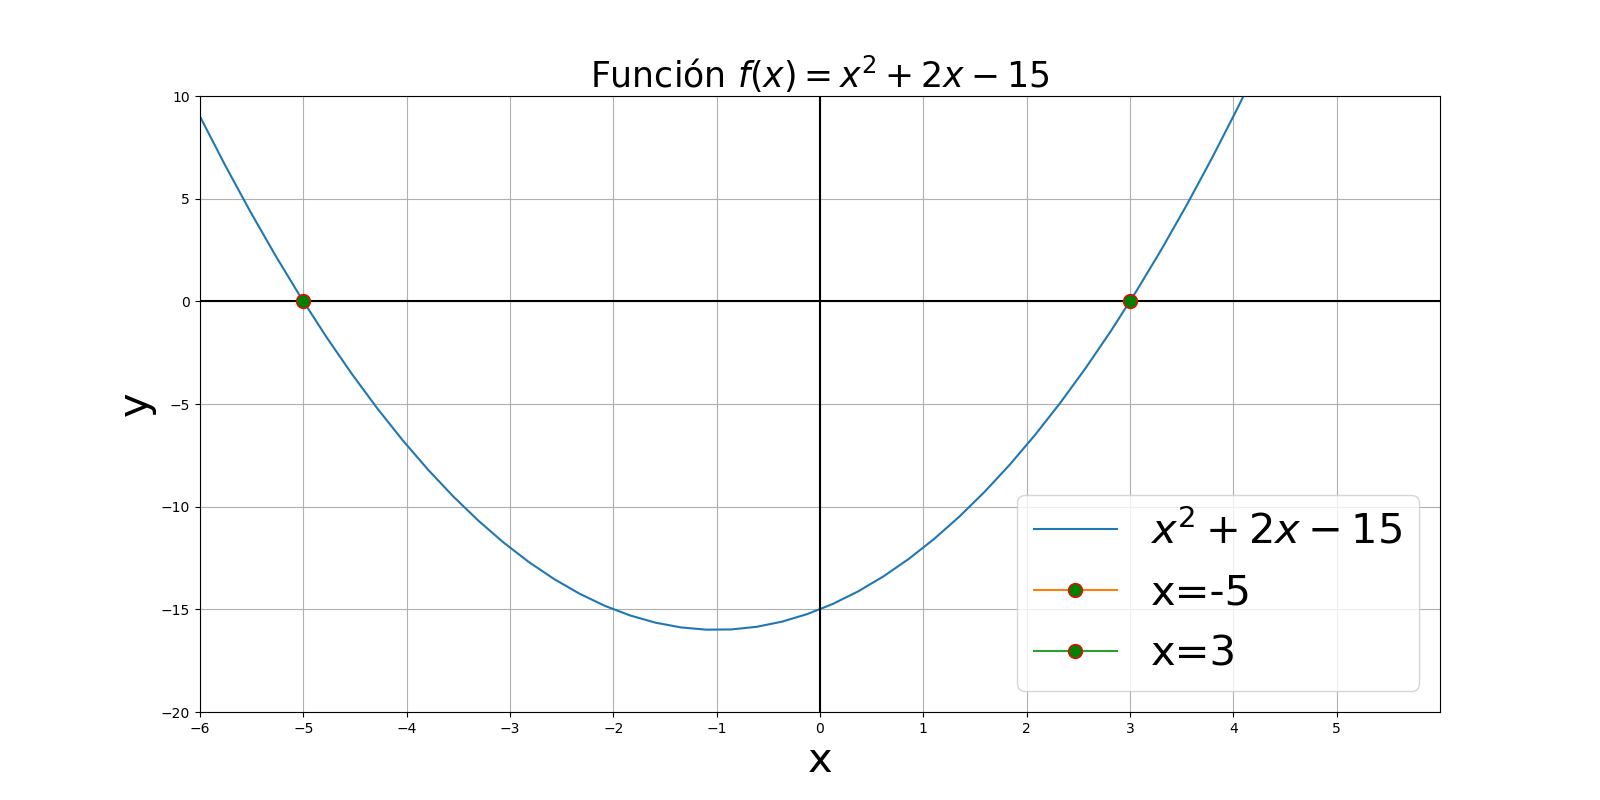
\includegraphics[scale=0.30]{cua441.png}
\caption[Gráfica de función cuadrática del ejemplo (\ref{ejem441}).]{Gráfica de función cuadrática del ejemplo (\ref{ejem441}). La expresión cuadrática tiene dos puntos de intersección con el eje $x$, que son justamente en donde cambia de signo los intervalos. }
\end{figure}
\end{center}
La desigualdad solicita que sea mayor que cero, por lo que los intervalos solución son $]-\infty,-5]\cup [3,+\infty[$. Los infinitos siempre son intervalos abiertos, en los otros casos lo determina el símbolo de la desigualdad (en este caso es un intervalo cerrado por el símbolo de la igualad).
\end{myexample}

Para las expresiones fraccionales con polinomios el procedimiento es análogo, pero hay que considerar que el denominador debe ser $\neq 0$.\\

\begin{myexample}
\label{ejemplo442}
Resolver la siguiente desigualdad fraccional:\\
\begin{eqnarray}
\dfrac{x+1}{x+3}+1&\leq &0 \\
\dfrac{x+1+x+3}{x+3} &\leq &0 \\
\dfrac{2x+4}{x+3}& \leq & 0 
\end{eqnarray} 
Los ceros son $x\neq-3$ y $x=-2$. Ahora se hace la tabla de signos con los ceros encontrados.\\
\begin{center}
\begin{table}[h!]
\centering
\begin{tabular}{|c|c|c|}
\hline
$-\infty$ a $-3$&$-3$ a $-2$& $-2$ a $+\infty$ \\
\hline
$x=-10$&$x=-2,5=-5/2$&$0$ \\
$\dfrac{(-)}{(-)}=+$&$\dfrac{(-)}{(+)}=-$&$\dfrac{(+)}{(+)}=+$ \\
\hline 
\end{tabular}
\caption[Tabla de signos de una inecuación fraccional.]{Tabla de signos de una inecuación fraccional.}
\end{table}
\end{center}
El intervalo que cumple con la condición de la desigualdad es $]-3,-2]$. Notar que el intervalo debe ser abierto en $-3$ y cerrado $-2$, o si no la desigualdad queda indefinida.
\end{myexample}

\begin{center}
\begin{figure}[h!]
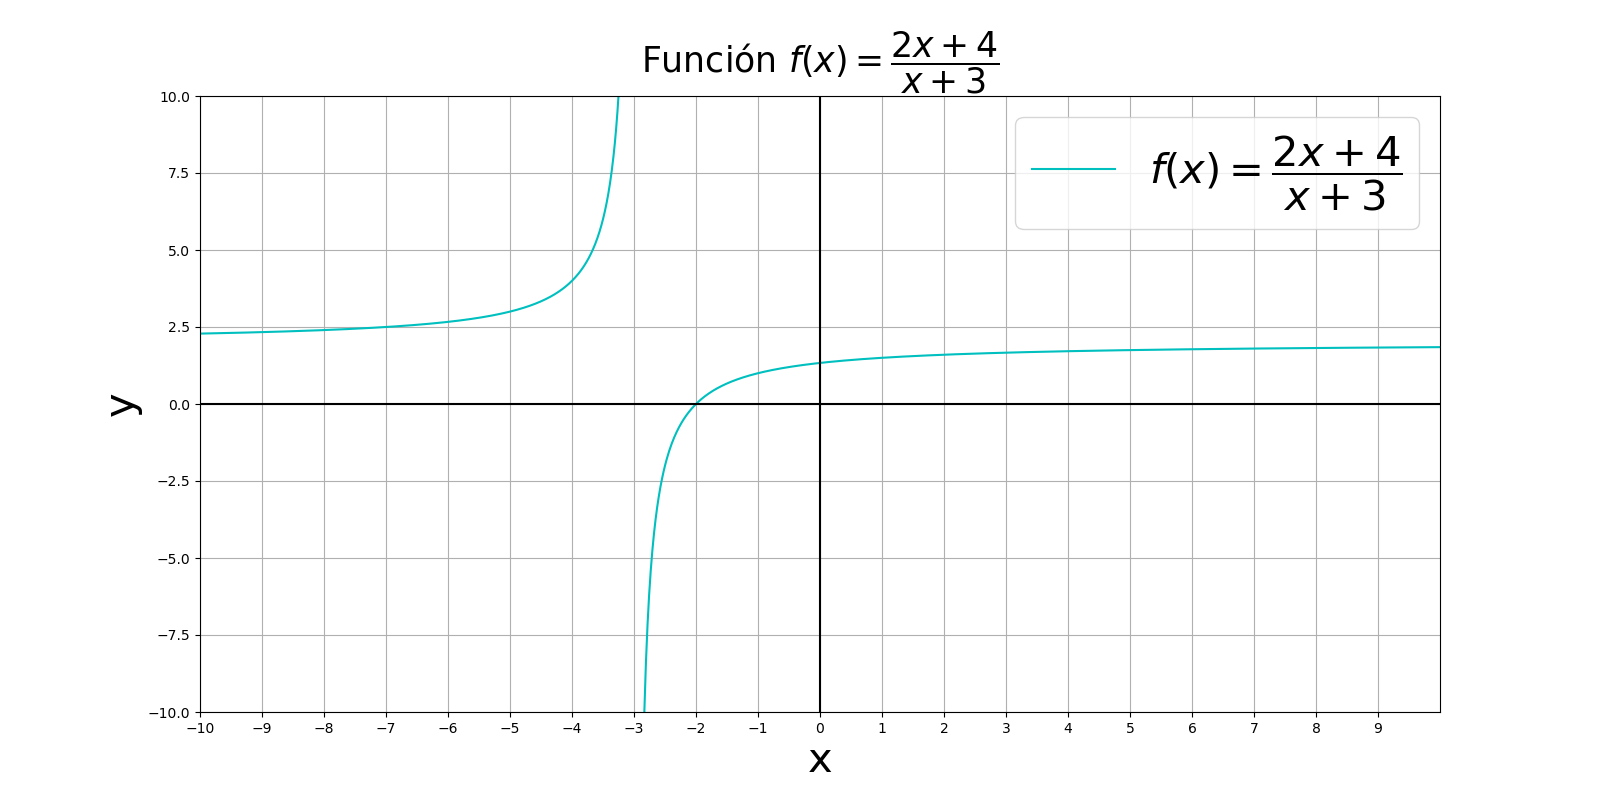
\includegraphics[scale=0.30]{inefracc0.png}\caption[Gráfico del ejemplo (\ref{ejemplo442}).]{Gráfico del ejemplo (\ref{ejemplo442}). Se Muestra (nuevamente) el intervalo en que la función cumple con la condición de la desigualdad (menor que cero, $\leq 0$).}
\end{figure}
\end{center}
\newpage
\subsection{Desigualdades polinomiales con valor absoluto}
Para finalizar el análisis de las desigualdades racionales, veremos el caso cuando tienen un valor absoluto. El procedimiento es el mismo solo que ahora se debe tener en consideración que habrán dos tablas con su (o sus) respectivo(s) conjunto(s) solución (o soluciones), que se deben unir. Luego, los conjuntos de las tablas se deberán intersectar o unir según el caso de valor absoluto. Ver el segundo ejercicio del ejemplo (\ref{ejemplodosd}).


\begin{myexample}
Resolver las siguientes expresiones polinomiales de fracciones con valor absoluto.\\

\noindent\textit{i)}
\begin{eqnarray*}
\left|\dfrac{1}{x}+3 \right| &\leq &3 \\
-3\leq &\dfrac{1}{x}+3& \leq 3 \\
-3\leq \dfrac{1}{x}+3 &\wedge &\dfrac{1}{x}+1 \leq 1 \\
0\leq \dfrac{1}{x}+6 &\wedge &\dfrac{1}{x} \leq 0\\
\underbrace{0\leq \dfrac{1+6x}{x}}_\text{$x\neq 0$,  $x=-1/6$} &\wedge &\underbrace{\dfrac{1}{x}\leq 0}_\text{$x\neq 0$}\\
\end{eqnarray*}

\begin{minipage}{0.5\textwidth}
\begin{tabular}{|c|c|c|}
\hline
  $-\infty$ a $-1/6$ & $-1/6$ a $0$ & $0$ a $+\infty$ \\
\hline
 $x=-10$ & $x-1/12$ & $x=10$  \\
  $\dfrac{(-)}{(-)}=+$&$\dfrac{(+)}{(-)}=-$&$\dfrac{(+)}{(+)}=+$  \\
\hline
\end{tabular}
\end{minipage}
\begin{minipage}{0.5\textwidth}
\begin{tabular}{|c|c|}
\hline
 $-\infty$ a $0$ & $0$ a $\infty$    \\
\hline
 $x=-1$&$x=1$   \\
  $\dfrac{(1)}{(-)}=-$& $\dfrac{(1)}{(+)}=+$  \\
  \hline
\end{tabular}
\end{minipage}

Ahora se debe hacer la intersección de ambas tablas, resultando como conjunto solución $\left( ]-\infty,-1/6]\cup ]0,+\infty[\right) \cap ]-\infty,0[=]-\infty,-1/6]$.\\
\begin{center}
\begin{figure}[h!]
\centering
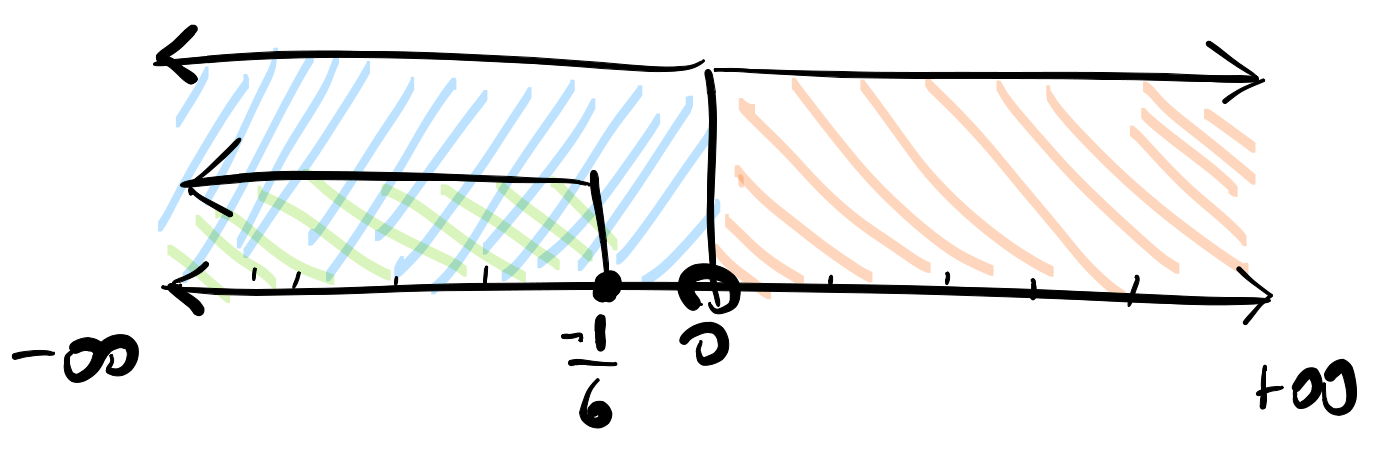
\includegraphics[scale=0.25]{Desabsfracc0.png}
\caption[Gráfica de los intervalos en la recta de los números reales.]{Gráfica de los intervalos en la recta de los números reales. Siempre se dibujan todos los  intervalos que cumplen la condición de la desigualdad (mayor o menor que 0).}
\end{figure}
\end{center}

\noindent\textit{ii)}\\
\begin{eqnarray*}
\left|\dfrac{3x-1}{x}\right| &\geq &4  \\
\dfrac{3x-1}{x}\geq 4 &\vee & \dfrac{3x-1}{x}\leq -4\\
\dfrac{3x-1}{x}-4\geq 0 &\vee & \dfrac{3x-1}{x}+4\leq 0\\
\dfrac{3x-1-4x}{x}\geq 0 &\vee & \dfrac{3x-1+4x}{x}\leq 0\\
\underbrace{\dfrac{-1-x}{x}\geq 0}_{x\neq 0, x=-1} &\vee & \underbrace{\dfrac{7x-1}{x}\leq 0}_{x\neq 0, x=1/7}
\end{eqnarray*}
\end{myexample}

\begin{minipage}{0.5\textwidth}
\begin{tabular}{|c|c|c|}
\hline
  $-\infty$ a $-1$ & $-1$ a $0$ & $0$ a $+\infty$ \\
\hline
 $x=-10$ & $x=-1/2$ & $x=10$  \\
  $\dfrac{(+)}{(-)}=-$&$\dfrac{(-)}{(-)}=+$&$\dfrac{(-)}{(+)}=-$\\
\hline
\end{tabular}
\end{minipage}
\begin{minipage}{0.5\textwidth}
\begin{tabular}{|c|c|c|}
\hline
 $-\infty$ a $0$ & $0$ a $1/7$& $1/7$ a $+\infty$    \\
\hline
 $x=-1$&$x=1/14$&$x=10$   \\
  $\dfrac{(-)}{(-)}=+$& $\dfrac{(-)}{(+)}=-$& $\dfrac{(+)}{(+)}=+$ \\
  \hline
\end{tabular}
\end{minipage}

En este caso debemos unir todos los resultados. De ambas tablas solo sirve un intervalo de cada una, entonces el conjunto solución es $[-1,0[\cup ]0,1/7]=[-1,1/7]-\{0\}$.

\begin{center}
\begin{figure}[h!]
\centering
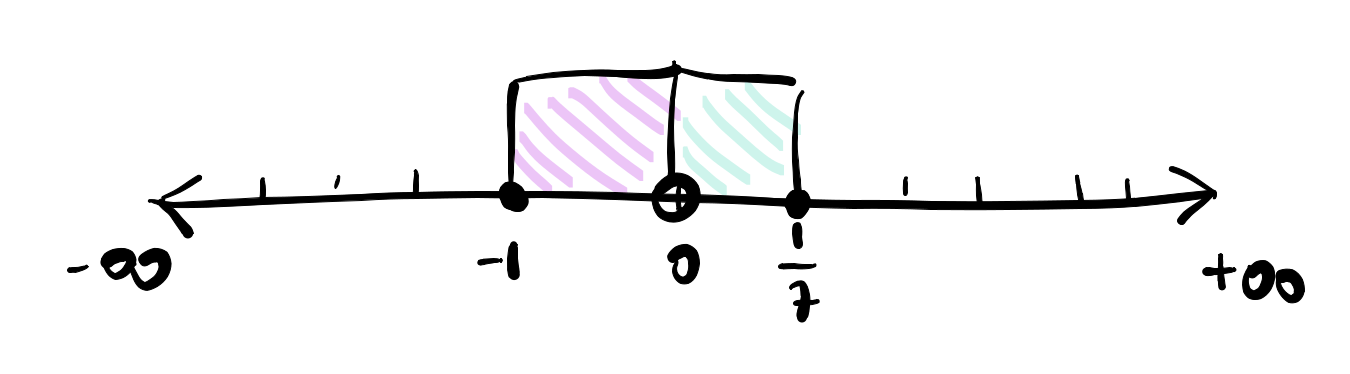
\includegraphics[scale=0.25]{Desabsfracc1.png}
\caption[Gráfica de los intervalos en la recta de los números reales.]{Gráfica de los intervalos en la recta de los números reales. Procedimiento similar al ejemplo anterior, solo que en este caso se debe unir los intervalos en vez de intersectarlos.}
\end{figure}
\end{center}
	\rhead[\thepage]{\scriptsize{CAPÍTULO \thechapter}. \rightmark}
\lhead[CAPÍTULO \thechapter. \leftmark]{}
%======================================================================
\chapter{Funciones matemáticas}
\label{FM}
\markboth{Funciones matemáticas}{Funciones matemáticas}
%======================================================================
Usualmente, se necesita agrupar elementos bajo ciertas condiciones como lo vimos en la sección (\ref{TC}). Ahora, hay ciertos grupos que tienen una correspondencia que asocia estos conjuntos, entonces se genera una dependencia del valor de un conjunto con respecto a otro, a esto se le llama \textit{función matemática}. 
\begin{mydef}
\textbf{Función matemática. }Una función de un conjunto $X$ a un conjunto $Y$ es una regla de correspondencia que asigna a cada elemento $x$ de $X$ exactamente un elemento $y$ de $Y$.
\end{mydef}

A las funciones se le acostumbra asignar letras como $f$, $g$ o $h$, pero puede ser cualquier letra o símbolo. La primera notación que usualmente se utiliza es $f:X\longrightarrow Y$ que nos dice desde donde y hasta donde va la función. En este caso va desde el conjunto $X$ que se llama \textit{dominio} hasta el conjunto $Y$ que se llama \textit{imagen} o \textit{recorrido}. La segunda forma de representar la función es $y=f(x)$, donde $y$ es un elemento de la imagen y $x$ es una elemento del dominio que se le aplicó la función $f()$.\\
La aplicación de una función se puede asemejar a un proceso que tiene entradas (los elementos $x$ del conjunto $X$), una función y salidas (los elementos $y$ del conjunto $Y$) con la función aplicada. Las entradas $x$ no dependen de nada previo, por lo que se les llama variables independientes y como las salidas $y$ dependen de las entradas se les llama variables dependientes.\\

La variable que aparece dentro del paréntesis en $f()$ es la que se reemplaza cada vez que aparezca la variable, es decir, si la función es $f()=()+3$ y uno desea saber la expresión de $f(j^{3})=j^{3}+3$.\\
\begin{myexample}
Evaluar una función con un elemento del dominio.
\begin{eqnarray*}
f(x)&=&x^{4}+3x^{2}+x+56\\
f(7)&=& (7)^{4}+3\cdot (7)^{2}+(7)+56=2611
\end{eqnarray*}
\end{myexample}

\begin{center}
\begin{figure}[h!]
\centering
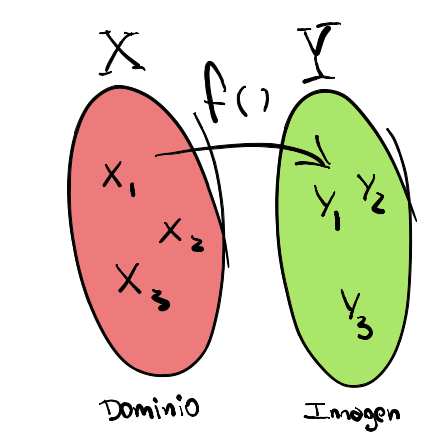
\includegraphics[scale=0.45]{function.png}
\caption[Esquema de una función matemática.]{Esquema de una función matemática. El óvalo rojo representa el dominio de la función que es un conjunto $X$ con los elementos $x_{1}$, $x_{2}$ y $x_{3}$. La flecha muestra la dirección de la función y la operación que se aplicará. El óvalo verde representa la imagen de la función de un conjunto $Y$ con elementos $y_{1}$, $y_{2}$ y $y_{3}$.}
\label{fn00}
\end{figure}
\end{center}

\begin{center}
\begin{figure}[h!]
\centering
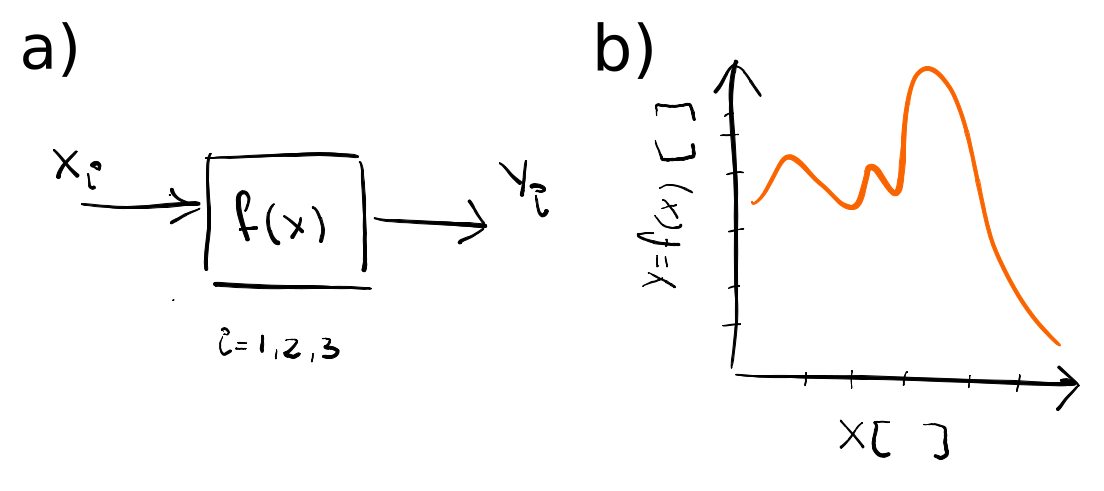
\includegraphics[scale=0.45]{function0.png}
\caption[Esquema de una función y gráfico de una variable dependiente e independiente.]{Esquema de una función y gráfico de una variable dependiente e independiente. a) Las variables $x_{i}$ representan las entradas de la función. Luego, la caja es donde se aplica la función $f(x)$ y finalmente se tiene una salida que son las variables $y_{i}$. b) Gráfica de una variable independiente, $x$, y una variable dependiente, $y$, que va cambiando su valor cuando se evalúa cada elemento del dominio (los $x_{i}$).}
\label{imagfx}
\end{figure}
\end{center}

%----------------------------------------------------------------------
\section{Dominio e imagen de una función}
\label{domim}
%----------------------------------------------------------------------
\begin{mydef}
\textbf{Dominio de una función.} El dominio de una función $f$ es el mayor subconjunto de números reales para los que $f(x)$ es un número real. Se denota $Dom(f(x))$.
\begin{eqnarray}
Dom(f(x))=\{x\in X|\exists y \in Y,f(x)=y\}
\end{eqnarray}
\label{domfx}
\end{mydef}
Entonces, el dominio de una función es el conjunto más grande donde está definida, por ejemplo $1/x$ está definido en para cualquier número real menos para el cero, por lo que el dominio de la función son todos los números reales menos el cero ($\mathbb{R}-\{0\}$). La imagen de la función son todos los valores que puede tomar $f(x)$.

\begin{mydef}
\textbf{Imagen de una función.} Es el conjunto $Y$ que tiene como elementos todos los posibles valores que puede tomar la función. Se denota como $Im(f(x))$.
\begin{eqnarray}
Im(f(x))=\{y\in Y|\exists x\in X,f(x)=y \}
\end{eqnarray}
\label{imfx}
\end{mydef}

\begin{myexample} Encontrar el dominio de las siguientes funciones:\\

\noindent\textit{i)}
\begin{eqnarray*}
f(x)&=&\sqrt{x+7}\\
Dom(f(x))&=& x+7\geq 0\\
Dom(f(x))&=& x\geq -7\\
Dom(f(x))&=& [-7,+\infty [
\end{eqnarray*}

\noindent\textit{ii)}
\begin{eqnarray*}
f(x)&=&\dfrac{1}{x^{2}-4}\\
Dom(f(x))&=& x^{2}-4\neq 0 \\
Dom(f(x))&=& x^{2}\neq 4 \\
Dom(f(x))&=& \sqrt{x^{2}}\neq \sqrt{4} \\
Dom(f(x))&=& |x|\neq 2 \\
Dom(f(x))&=& x\neq \pm 2 \\
Dom(f(x))&=& \mathbb{R}-\{-2,+2\}
\end{eqnarray*}
\end{myexample}

Para calcular el dominio de una función no hay un procedimiento único, por lo que se debe analizar el tipo de función que tenemos y que no se anule para que tome siempre valores reales. Por ejemplo, en el caso de las raíces cuadradas se debe cumplir que el radicando debe ser mayor que cero o para el caso de las expresiones fraccionales, el denominador debe ser distinto de cero. A continuación cual es el dominio de cierto tipo de funciones.

\begin{itemize}
	\item Funciones polinomiales: El dominio son todos los números reales.
	\begin{eqnarray*}
	f(x)&=&4x^{7}+50x^{25}+2\\
	Dom(f(x))&:& \mathbb{R}
	\end{eqnarray*}
	\item Función racional (fracciones): Son todos los números reales, menos los valores que hace cero al denominador.
	\begin{eqnarray*}
	f(x)&=&\dfrac{1}{x+2}\\
	Dom(f(x))&:&\mathbb{R}-\{-2\}
	\end{eqnarray*}
	\item Funciones radicales con índice par: El dominio son todos los valores que hacen que el radicando sea mayor que cero.
	\begin{eqnarray*}
	f(x)&=&\sqrt{3x+7}\\
	Dom(f(x))&:& \left[\dfrac{-7}{3},+\infty \right[
	\end{eqnarray*}
	\item Funciones radicales con índice impar: Es el dominio del radicando, no está sujeta a una desigualdad.
	\begin{eqnarray*}
	f(x)&=&\sqrt[3]{7x+3}\\
	Dom(f(x))&:& \mathbb{R}
	\end{eqnarray*}
	\item Función logarítmica: El dominio está formado por todos los valores que hacen que el argumento del logaritmo sea mayor que cero.
	\begin{eqnarray*}
	f(x)&=&log\left(2x^{2}+3x+1\right)\\
	Dom(f(x))&:& \left]-\infty ,-1\right[ \cup \left]-\dfrac{1}{2},\infty \right[
	\end{eqnarray*}
	\item Función exponencial: El dominio son todos los reales, excepto los valores que anulan a la función que está en el exponente.
	\begin{eqnarray*}
	f(x)&=&e^{x}\\
	Dom(f(x))&:&\mathbb{R}
	\end{eqnarray*}
	\begin{eqnarray*}
	f(x)&=&e^{1/x}\\
	Dom(f(x))&:&\mathbb{R}-\{0\}
	\end{eqnarray*}
\end{itemize}

\section{Gráficas de una función}
Al momento de plasmar una función cualquiera debemos juntar las definiciones de dominio (\ref{domfx}), imagen (\ref{imfx}) y la figura (\ref{imagfx}), con estos tres elementos podemos graficar una función. Cada punto de la gráfica tiene la forma $(x_{i},y_{i})$ o $(x_{i},f(x_{i}))$, por lo que el eje $x$ representa el dominio de la función y el eje $y$ la imagen. \\
La función para un valor $y$ puede tener más de un valor en $x$, por ejemplo en $x^{2}$. No se puede dar el caso inverso, es decir, que por un valor de $x$ la función tenga dos o más valores en el $y$, es por ello que si uno traza una línea vertical en las gráficas, esta línea debe tocar solo un punto del gráfico, si no, no es una función.\\

\begin{center}
\begin{figure}[h!]
\centering
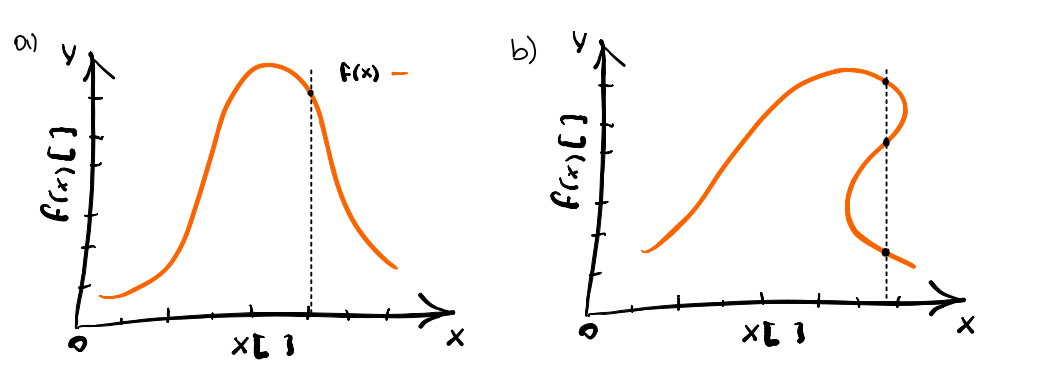
\includegraphics[scale=0.5]{lineafn.png}
\caption[Gráfica para diferenciar una función.]{Gráfica para diferenciar una función. a) Es una gráfica que muestra una línea vertical que toca en un solo punto a la gráfica, por lo tanto, es una función. b) La gráfica no es una función, ya que la línea toca a la función en tres puntos.}
\label{difx}
\end{figure}
\end{center}
Si la línea solo debe tocar en un punto, entonces ¿Qué ocurre cuando se grafica un círculo? En casos de círculos o elipses son dos funciones que al momento de graficarlas al mismo tiempo forman la figura. Por ejemplo, las gráficas que forman un círculo de radio 3 son $y=\pm\sqrt{9-x^{2}}$. 

\subsection{Intersecciones con los ejes}
Una de las formas más rápidas de obtener información de la gráfica de la función es ver en que puntos pasa por los ejes, se debe ver que para las intersecciones en el eje $y$ son de la forma ($0,f(0)$) mientras que para los del eje $x$ son ($x,0$). De esto se desprende que hay ciertos valores de $x$ que hacen que $y=0$, entonces el objetivo es encontrar esos $x$ que hace que $f(x)=0$. \\
Cuando se encuentran esos números se le llaman \textit{raíces} o \textit{soluciones} de la función que satisfacen la ecuación $f(c)=0$, siendo $c$ los números reales que son solución de la función.\\

Como se puede notar no siempre las funciones pasan por los ejes, hay casos en que la función toca en un solo punto, pero no cruza, a esto se llama una gráfica \textit{tangente} al eje. La función solo puede pasar o tocar al eje $y$ en un solo punto, siempre y cuando el $0$ esté en el dominio de la función.\\ 

\begin{center}
\begin{figure}[h!]
\centering
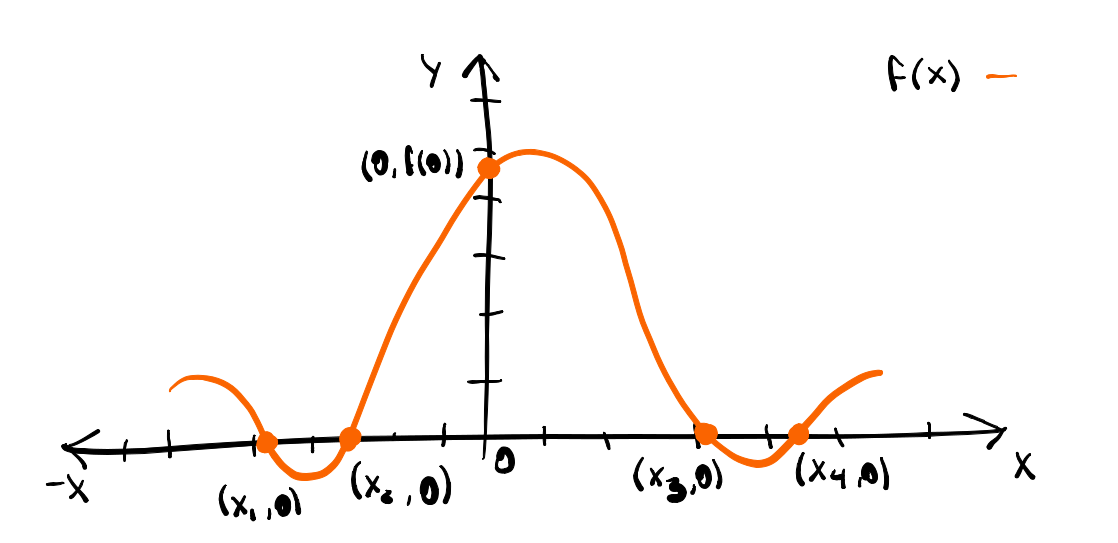
\includegraphics[scale=0.35]{interfn.png}
\caption[Función que intersecta los ejes.]{Función que intersecta los ejes. La función intersecta en 5 puntos y a los que pasan por el eje $x$ se les denomina ceros de la función. }
\label{interfx}
\end{figure}
\end{center}

\subsection{Simetrías y transformaciones }
El primer paso fue encontrar los puntos de intersección con los ejes, lo siguiente es identificar ciertos tipos de funciones para ver de forma rápida su gráfica en el plano. Hay ciertas funciones que tienen una invarianza\footnote{Es algo que no cambia al aplicarle una transformación.} que la llamaremos \textit{simetrías}. Todo esto al momento de ver la gráfica se ve que la función tiene un eje de simetría con respecto a un eje o recta.\\
Por la figura (\ref{imagfx}) se ve que la función solo puede tener simetría con respecto al eje $y$ (o una traslación del mismo), porque en caso contrario no sería una función. Esta simetría se puede clasificar en dos tipos, funciones \textit{pares} e \textit{impares}.
\begin{mydef}
\textbf{Funciones pares e impares.} Sea $x$ y $-x$ elementos perteneciente al dominio de la función $f(x)$. Se dice que:\\
\noindent i) Una función $f$ es par si $f(-x)=f(x)$.\\
\noindent ii) Una función $f$ es impar si $f(-x)=-f(x)$.\\
\end{mydef}


\begin{myexample}
Funciones pares e impares:\\

\noindent i) Función par:\\
\begin{eqnarray*}
f(x)&=&x^{2}\\
f(-2)&=&(-2)^{2}=4\\
f(2)&=&(2)^{2}=4\\
f(x)&=&f(-x)\\
\end{eqnarray*}
\noindent ii) Función impar:\\
\begin{eqnarray*}
f(x)&=&x^{3}\\
f(-2)&=&(-2)^{3}=-8\\
f(2)&=&(2)^{3}=8\\
f(x)&=&-f(x)
\end{eqnarray*}
\end{myexample}

\begin{center}
\begin{figure}[h!]
\centering
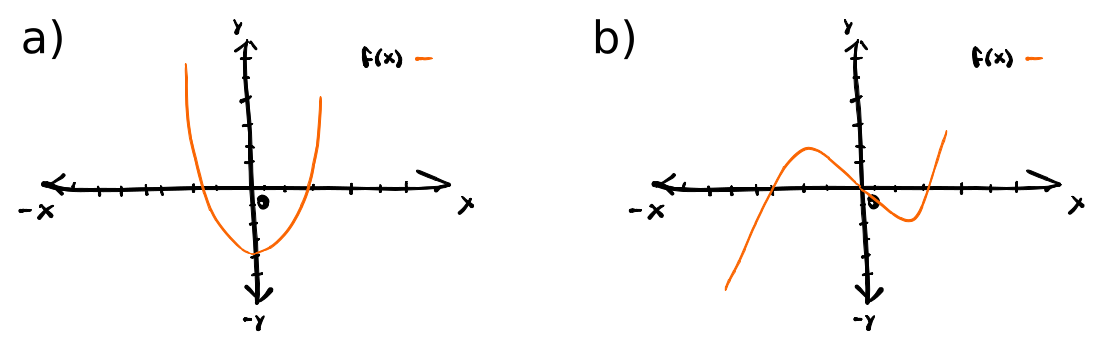
\includegraphics[scale=0.5]{parimpar.png}
\caption[Función par e impar.]{Función par e impar. a) Muestra una parábola que es una función par, es decir, los puntos ($x,y$) y (-$x,y$) son parte de la gráfica. b) Muestra una función impar, es decir, que los puntos ($x,y$) y ($-x,-y$) son parte de la gráfica.}
\label{parimparfx}
\end{figure}
\end{center}

\begin{mydef}
\textbf{Simetría.}\\

\noindent i) Una función $f$ es par si y sólo si su gráfica es simétrica respecto al $y$. \\
\noindent ii) Una función $f$ es impar si y sólo si su gráfica es simétrica respecto al origen.\\
\end{mydef}

\subsection{Transformaciones rígidas}
Este tipo de transformaciones es cualquiera que mueve la gráfica por el plano, pero no cambia la forma, es decir, son todo tipo de traslaciones de la función.\\

\begin{mydef}
\textbf{Transformaciones rígidas: Desplazamientos verticales y horizontales.} Sea $f(x)$ una función definida en los números reales y $c$ una constante real mayor que cero ($c>0$), entonces, las gráficas se someten a las siguientes traslaciones:\\

\noindent i) $y=f(x)+c$ es la gráfica desplazada verticalmente en $c$ hacia arriba.\\

\noindent ii) $y=f(x)-c$ es la gráfica desplazada verticalmente en $c$ hacia abajo.\\

\noindent iii) $y=f(x+c)$ es la gráfica desplazada horizontalmente en $c$ unidades hacia la izquierda.\\

\noindent iv) $y=f(x-c)$ es la gráfica desplazada horizontalmente en $c$ unidades hacia la derecha.\\
\end{mydef}

Se puede combinar estas traslaciones, que en el gráfico sería trasladar en \textit{diagonal} a la función y con las fórmulas de la definición anterior es $y=f(x\pm c)\pm c$.

\begin{center}
\begin{figure}[h!]
\centering
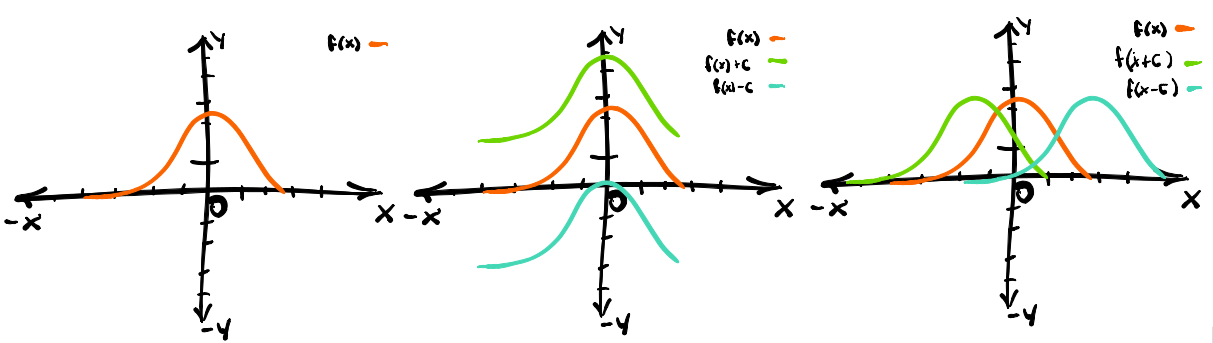
\includegraphics[scale=0.5]{trasfn.png}
\caption[Transformaciones rígidas.]{Transformaciones rígidas. a) Es la función original. b) Muestra la función original (linea naranja) y sus traslaciones verticales en $c$ unidades. c) Muestra la función original y sus respectivas traslaciones horizontales en $c$ unidades.}
\label{trasfx}
\end{figure}
\end{center}

\begin{mydef}
\textbf{Reflexiones.} Sea $f(x)$ una función definida en los números reales, entonces:

\noindent i) $y=-f(x)$ es la gráfica de $f(x)$ reflejada en el eje $x$.\\
\noindent ii) $y=f(-x)$ es la gráfica de $f(x)$ reflejada en el eje $y$. \\
\end{mydef}
%ejemplos 
\subsection{Transformaciones no rígidas}
A diferencia de la subsección anterior, ahora si se modificará la forma de la función original. Ahora, la función se puede achatar, estirar o en otros casos cambiar la pendiente.
\begin{mydef}
\textbf{Transformaciones no rígidas: Estiramientos y compresiones verticales.} Sea $f(x)$ una función definida en los números reales, entonces la gráfica de $y=c\cdot f(x)$ es:\\

\noindent i) Estirada verticalmente por un factor de $c$ unidades, si $c>1$.\\

\noindent ii) comprimida verticalmente por un factor de $c$ unidades, si $0<c<1$.\\
\end{mydef}

\begin{center}
\begin{figure}[h!]
\centering
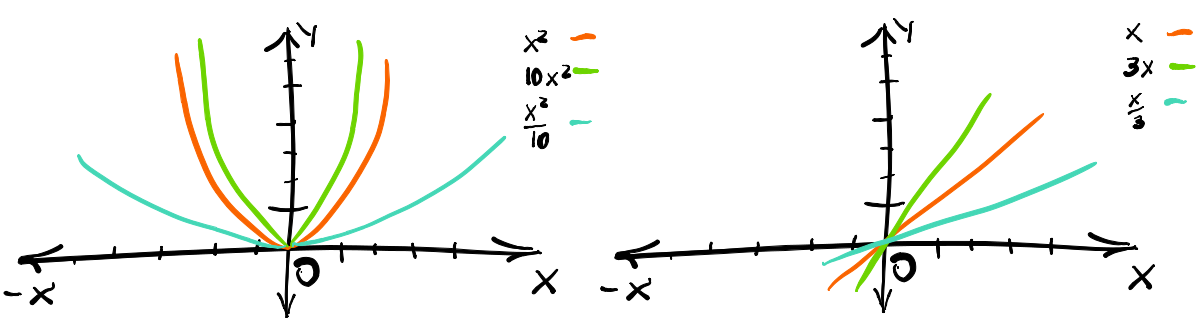
\includegraphics[scale=0.35]{deforfn.png}
\caption[Transformaciones no rígidas.]{Transformaciones no rígidas. Se ven las posibilidades de deformar la función $f(x)$ cambiando su forma, para el gráfico de la izquierda es una función cuadrática con forma $y=a_{2}x^{2}$ y el de la derecha es una función lineal de la forma $y=a_{1}x+a_{0}$. La definición de coeficientes se ve en la ecuación (\ref{polg00}).}
\label{deforfx}
\end{figure}
\end{center}

\section{Función cuadrática y lineal}
\label{fnlincua}
Anteriormente vimos a los polinomios y su forma más general (ver la ecuación  \ref{polg00}), entonces ahora veremos algunos casos particulares. Recordando la fórmula de un polinomio con un exponente $n$ que es entero y no negativo
\begin{eqnarray}
f(x)=a_{n}x^{n}+a_{n-1}x^{n-1}+\cdots +a_{2}x^{2}+a_{1}x+a_{0}
\label{polfn}
\end{eqnarray}
De (\ref{polfn}) desprenderemos tres casos. La constante es cuando $a_{0}\neq 0$, el caso lineal es cuando $a_{0},a_{1}\neq 0$ y el caso cuadrático es cuando $a_{0},a_{1}, a_{2}\neq 0$.

\begin{mydef}
\textbf{Funcionales polinomiales.} Sea $f(x)$ una función polinomial definida en los números reales, se desprenden los siguientes casos:\\

\noindent i) Si $f(x)=a$ es una función constante.\\
\noindent ii) Si $f(x)=ax+b$ es una función lineal.\\
\noindent iii) Si $f(x)=ax^{2}+bx+c$ es una función cuadrática.\\

Los coeficientes $a_{0}$, $a_{1}$ y $a_{2}$ fueron redefinidos por simplicidad, pero no se pierde generalidad.\\
\end{mydef}

\subsection{Función lineal}
Ya tuvimos una aproximación con este tipo de cuentas y lucen como el gráfico a la derecha de la figura (\ref{deforfx}). El caso más simple es cuando la recta pasa por el origen, por lo que la función luce de la forma $f(x)=ax$. El coeficiente $a$ nos da la pendiente de la recta, es decir, si $a$ negativo la recta cambia su sentido.\\

El dominio de estas funciones (y el de todas las funciones polinomiales que no son fracciones) son todos los números reales, porqué en ningún caso se indetermina la expresión.
\begin{myexample}
Muestra de algunas ecuaciones lineales:\\

\noindent i) $f(x)= x-2$ \\
\noindent ii) $f(x)=x $\\
\noindent iii) $f(x)= x+2 $\\
\noindent iv) $f(x)= -x$ \\

\begin{center}
\begin{figure}[h!]
\centering
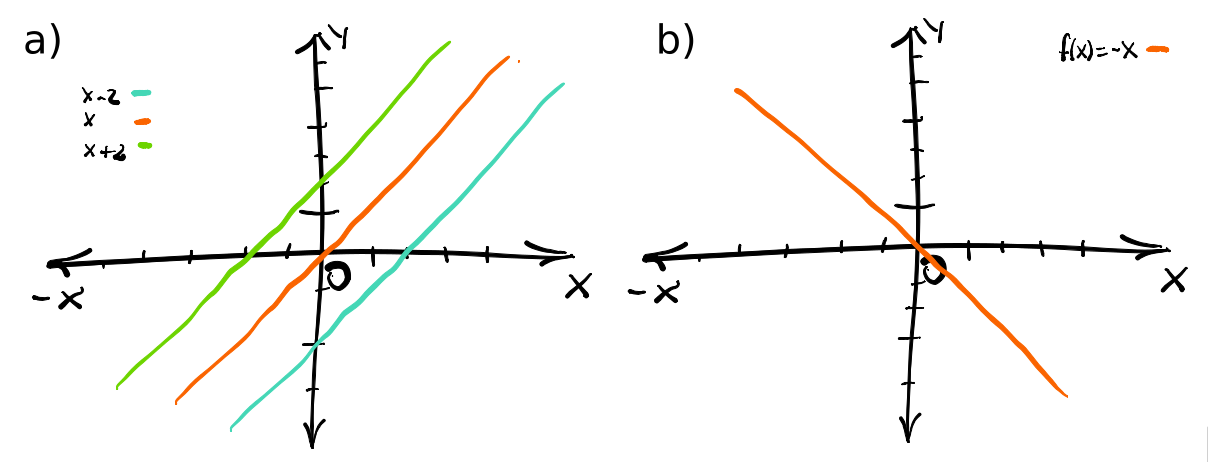
\includegraphics[scale=0.5]{linfn.png}
\caption[Funciones lineales.]{Funciones lineales. a) Ejemplo de tres funciones lineales, la recta naranja grafica la función $ii$ y las otras dos rectas son la misma función pero desplazadas (caso $i$ y $ii$). b) Gráfica de la recta $f(x)=-x$ que da muestra que el factor que acompaña a $x$ es la pendiente de la recta.} \label{linfn}
\end{figure}
\end{center}
\end{myexample}


\subsection{Función cuadrática}
Subiendo de $n$ en las funciones polinomiales nos encontramos con el caso cuadrático, usualmente llamado parábola. El caso mas simple es $f(x)=ax^{2}$, pero el caso más general tiene deformaciones y traslaciones que la dejan de la forma $f(x)=ax^{2}+bx+c$.\\
Si el coeficiente $a<0$ la parábola es un reflejo de $ax^{2}$ con $a>0$, o lo que se dice frecuentemente que \textit{apunta hacia abajo}. El coeficiente $c$ es el que desplaza horizontal o verticalmente la gráfica.\\
\newpage
\begin{myexample}
Muestra de algunas ecuaciones cuadráticas:\\

\noindent i) $f(x)= x^{2}-2$ \\
\noindent ii) $f(x)=x^{2} $\\
\noindent iii) $f(x)= x^{2}+2 $\\
\noindent iv) $f(x)= -x^{2}$ \\

\begin{center}
\begin{figure}[h!]
\centering
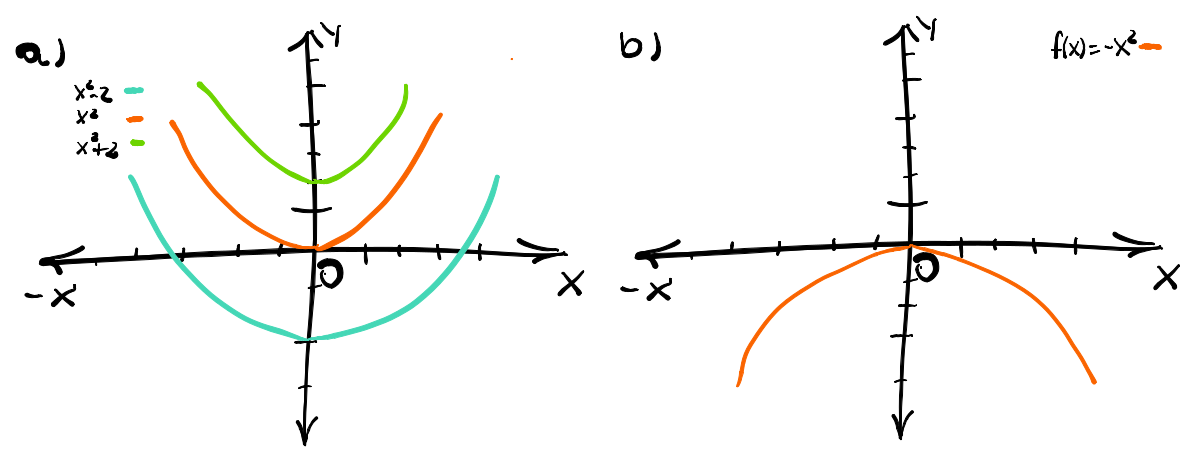
\includegraphics[scale=0.5]{cuafn.png}
\caption[Funciones cuadraticas.]{Funciones cuadráticas. a) Gráfica de funciones cuadráticas desplazadas con respecto a la función original $f(x)=x^{2}$. b) Gráfica de la función parabólica de $f(x)=-x^{2}$ que es el reflejo con respecto al eje $x$ de $x^{2}$. } \label{cuadfn}
\end{figure}
\end{center}
\end{myexample}


\subsubsection{Vértice y eje}
Los puntos que caracterizan a una parábola son el signo de $a$ para ver hacia donde crece, los posibles puntos de intersección con el eje $x$ y su vértice. La parábola puede estar apuntando hacia arriba ($a>0$) o hacia abajo ($a<0$), el punto más abajo ($a>0$) o más arriba ($a<0$) se llama vértice. Este punto marca la mitad de la parábola, que al hacer una línea en $x=h$ marca el eje de simetría. La forma matemática de obtener el vértice de una parábola cualquiera es la siguiente:\\
\begin{eqnarray}
f(x)=a(x-h)^{2}+k,\label{eqver}
\end{eqnarray}
ahora modificaremos el polinomio de segundo grado para compararlos con (\ref{eqver}).
\begin{eqnarray}
f(x)&=& ax^{2}+bx+c\nonumber\\
f(x)&=& a\left(x^{2}+\dfrac{b}{a}x \right)+c\nonumber\\
f(x)&=& a\left(x^{2}+\dfrac{b}{a}x-\dfrac{b^{2}}{4a^{2}}+\dfrac{b^{2}}{4a^{2}}  \right)+c\nonumber\\
f(x)&=& a\left(x^{2}+\dfrac{b}{a}x+\dfrac{b^{2}}{4a^{2}} \right)-\dfrac{b^{2}}{4a} +c\nonumber\\
f(x)&=& a\left(x+\dfrac{b}{2a} \right)^{2}+\dfrac{4ac-b^{2}}{4a} \label{eqver0}
\end{eqnarray}
Luego, se compara término a término entre las ecuaciones (\ref{eqver}) y (\ref{eqver0}), por lo que el vértice y el eje quedan definidos como:\\
\begin{eqnarray*}
h=\dfrac{-b}{2a}\hspace{6px}y\hspace{6px}k=\dfrac{4ac-b^{2}}{4a}
\end{eqnarray*}
En consecuencia el vértice de la parábola $(h,k)$. El punto del vértice es:
\begin{eqnarray}
\left(-\dfrac{b}{2a},f\left(-\dfrac{b}{2a} \right) \right)
\end{eqnarray}

Notar que para llegar a la ecuación (\ref{eqver0}) se realizó la operación de completar cuadrado (Para ver en detalle el completar cuadrado revisar el apéndice \ref{completarbi}). Consiste en sumar y restar un mismo termino, es decir, un cero para que quede un cuadrado de binomio de la forma $(a+b)^{2}$ más un término.  

\subsubsection{Intersección con los ejes}
Para encontrar los puntos en que la parábola pasa por los ejes utilizaremos un concepto ya visto, la soluciones de la ecuación de segundo grado. En la ecuación (\ref{raicesseg}) se ven las dos soluciones, que son justamente los dos puntos donde la parábola toca el eje $x$.\\ 
\begin{eqnarray}
x_{+}=\dfrac{-b+\sqrt{b^{2}-4ac}}{2a} \hspace{6px}y\hspace{6px}x_{-}=\dfrac{-b-\sqrt{b^{2}-4ac}}{2a}
\label{raicesseg}
\end{eqnarray}
Los puntos $x_{+}$ y $x_{-}$ son los que muestran las intersecciones con el eje $x$.

\begin{myexample}
Encontrar las intersecciones y el vértice de la siguiente función:
\begin{eqnarray*}
f(x)&=& x^{2}+2x-3\\
f(x)&=& (x+1)(x-3)\\
x=-1 &y& x=3\\
(-1,0) &y& (3,0)\\
\end{eqnarray*}
Para el vértice se debe completar cuadrados para igualar $f(x)$ con la ecuación (\ref{eqver}).
\begin{eqnarray*}
f(x)&=& x^{2}-2x-3\\
f(x)&=& x^{2}-2x+1-1-3\\
f(x)&=& (x^{2}-2x+1)-4\\
f(x)&=& (x-1)^{2}-4\\
f(x)&=& a(x-h)^{2}+k\\
\end{eqnarray*}
Al comparar los términos se obtiene que el vértice de la parábola está en el punto $(1,-4)$.
\end{myexample}

\section{Funciones crecientes y decrecientes}
\label{funcrede}
Hemos visto en las figuras (\ref{deforfx}), (\ref{linfn}) y (\ref{cuadfn}) un comportamiento de las funciones que aumentan y disminuyen por tramos. Cuando la función se mantiene en una tendencia de crecer o decrecer se clasifican en los siguientes casos:
\begin{mydef}
\textbf{Funciones crecientes y decrecientes.} Sea $f(x)$ una función real que está definida en un intervalo con extremos $x_{1}$ y $x_{2}$, que son dos números cualesquiera tales que $x_{1}<x_{2}$. Entonces, se cumple lo siguiente:\\

\noindent i) La función $f(x)$ es creciente en el intervalo si, $f(x_{1})<f(x_{2})$. \\
\noindent ii) La función $f(x)$ es decreciente en el intervalo si, $f(x_{1})>f(x_{2})$.  \\

\begin{center}
\begin{figure}[h!]
\centering
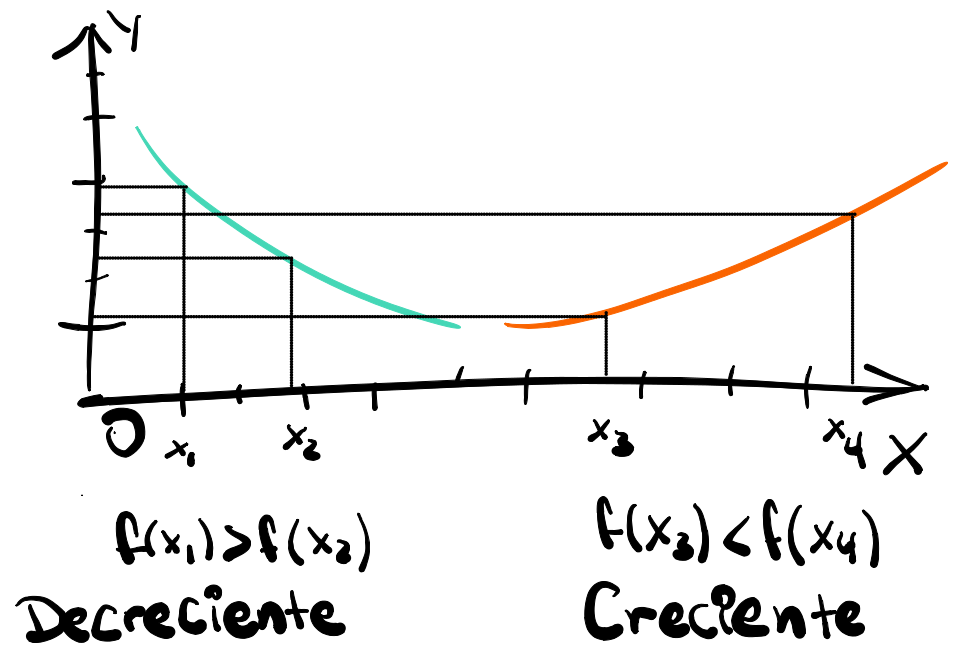
\includegraphics[scale=0.30]{credrefn.png}
\caption[Funciones crecientes y decrecientes.]{Funciones crecientes y decrecientes. .} \label{credrefn}
\end{figure}
\end{center}
\end{mydef}

Esta clasificación es una primera herramienta para saber como se comporta la función y consiste en seleccionar dos elementos del dominio para ver la respectiva imagen. Se debe considerar que una herramienta más poderosa se verán más adelante en el capítulo de calculo infinitesimal.

\begin{myexample}
Sean las funciones $f(x)=x^{2}$ y $g(x)=-x^{2}$ definida en los números reales. Seleccione dos elementos del dominio y mencione si es creciente o decreciente.\\

i) $f(x)=x^{2}$:\\
\begin{eqnarray*}
f(x_{1})&=& f(x_{1}=3)=f(3)=3^{2}=9\\
f(x_{2})&=& f(x_{2}=4)=f(4)=4^{2}=16
\end{eqnarray*}
$x_{2}>x_{1}$, por lo que $f(x)$ es una función creciente en este intervalo. \\

i) $g(x)=-x^{2}$:\\
\begin{eqnarray*}
f(x_{1})&=& f(x_{1}=3)=f(3)=-3^{2}=-9\\
f(x_{2})&=& f(x_{2}=4)=f(4)=-4^{2}=-16
\end{eqnarray*}
$x_{2}<x_{1}$, por lo que $g(x)$ es una función decreciente en este intervalo. \\
\end{myexample}
Si los valores coinciden para ambos $x$, entonces es una función constante.
\newpage
\section{Funciones por partes}
Como el nombre lo dice, es una función que según el tramo del dominio que uno seleccione va a tener una función diferente. El primer acercamiento es el valor absoluto, que en su versión mas simple son dos rectas con pendientes opuestas (ver la definición \ref{absdef}).\\

\begin{myexample}
\textbf{Función por tramos}. Cantidades de medicina (mg) contra la alergia según la edad del paciente (años):\\
%\begin{center}
%\begin{table}[h!]
%\centering
%\begin{tabular}{|c|c|}
%\hline
%Bajo $6$ años de edad &Preguntar al Doctor \\
%\hline
%De $6$ a $12$ años& $12,5$ a $25$ $mg$ \\
%\hline
%De $12$ años hacia arriba & $25$ a $50$ $mg$\\
%\hline
%\end{tabular}
%\caption[Tabla de medicina anti alergia según la edad.]{Tabla de medicina anti alergia según la edad.}
%\end{table}
%\end{center}
%Esta tabla se puede pasar a una función por tramos 

$$ f(x)= \left\{\begin{array}{ll}
Preguntar\hspace{3px} al\hspace{3px} doctor&,\hspace{2px} si\hspace{6px}0\leq x< 6\\
\dfrac{6x}{12,5}+19,24 &,\hspace{2px} si \hspace{6px}  6\leq x< 12\\ 
\dfrac{87x}{25}-16,76 &,\hspace{2px} si \hspace{6px} x \geq12
\end{array} \hspace{6px} \right.$$
El dominio de la función es rango etario que se considere (el x), mientras que la imagen son los miligramos de medicamentos.
\end{myexample}

\begin{myexample}
Se da un modelo simple\cite{Cancer} para ver si hay o no presencia de un tumor. Sea $M_{1}$, $M_{2},...,$ $M_{n}$ denota la alteración genética de interés. Esta alteración puede ser un punto de mutación, ganancia o perdida de una región cromosómica u otro evento genético. $N$ independientes especímenes (``tumores'') son obtenidos y la presencia o ausencia de la alteración de interés es guardad como un vector binario\footnote{Solo tiene dos resultados, en este caso es $0$ o $1$.} $x_{j}=\{x_{j1},x_{j2},...,x_{jn}\}$, donde: \\

	\begin{eqnarray*}
 x_{jl}= \left\{\begin{array}{ll}
0&,\hspace{4px} si\hspace{3px}en\hspace{3px}el\hspace{3px}j-esimo\hspace{3px}hay \hspace{3px}ausencia\hspace{3px}de\hspace{3px}alteraci\acute{o}n\hspace{3px}M_{l}\\
1 &,\hspace{4px} si\hspace{3px}en\hspace{3px}el\hspace{3px}j-esimo\hspace{3px}hay \hspace{3px}presencia\hspace{3px}de\hspace{3px}alteraci\acute{o}n\hspace{3px}M_{l}\\ 
				\end{array} \hspace{6px} \right.
	\end{eqnarray*}
	
Si tenemos por ejemplo el vector $x_{1}=\{x_{11},x_{12},..,x_{1n}\}$, ahora se debe calcular cada elemento del vector con la función por partes, por ejemplo si tomamos el primer elemento $x_{11}$.\\

	\begin{eqnarray*}
 x_{11}= \left\{\begin{array}{ll}
0&,\hspace{4px} si\hspace{3px}en\hspace{3px}el\hspace{3px}j-esimo\hspace{3px}hay \hspace{3px}ausencia\hspace{3px}de\hspace{3px}alteraci\acute{o}n\hspace{3px}M_{1}\\
1 &,\hspace{4px} si\hspace{3px}en\hspace{3px}el\hspace{3px}j-esimo\hspace{3px}hay \hspace{3px}presencia\hspace{3px}de\hspace{3px}alteraci\acute{o}n\hspace{3px}M_{1}\\ 
				\end{array} \hspace{6px} \right.
	\end{eqnarray*}
	
El dato de $0$ o $1$ estará dado por los datos recolectados de la muestra $M_{1}$, entonces una ejemplo del vector binario es $x_{j}=\{x_{j1},x_{j2},...,x_{jn}\}=\{0,1,0,...,0\}$.
\end{myexample}


\begin{myexample}
Graficar la siguiente función por tramos:
\begin{eqnarray*}
 f(x)= \left\{\begin{array}{ll}
-1&, x< 0\\
0 &, x=0\\ 
x+1 &, x>0 \\
\end{array} \hspace{6px} \right.
\end{eqnarray*}

\begin{center}
\begin{figure}[h!]
\centering
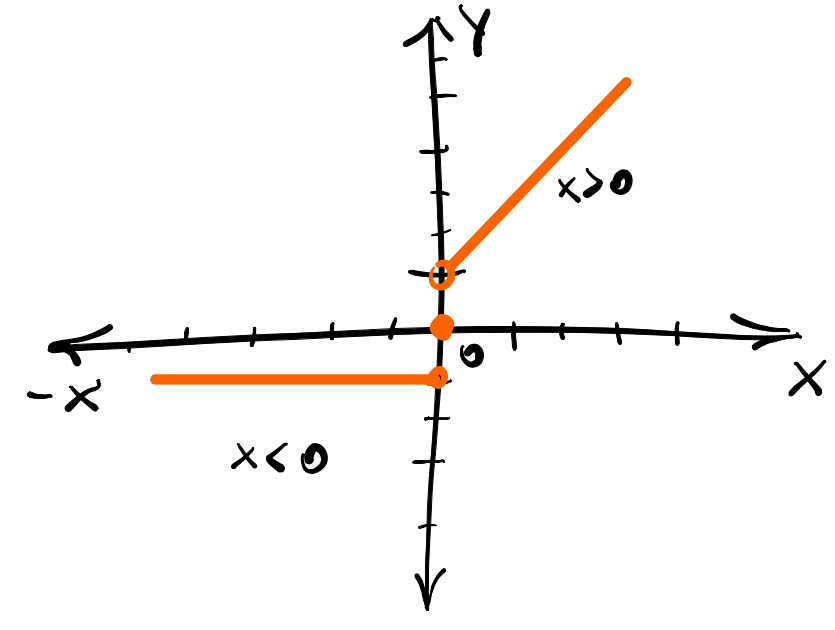
\includegraphics[scale=0.3]{partefn.png}
\caption[Función por partes.]{Función por partes. Son tres funciones, la primera es una función constante, la segunda un punto y la tercera es una recta. Notar que los extremos de la primera y tercera función consideran los extremos (por eso los círculos sin pintar). } \label{partefn}
\end{figure}
\end{center}
\end{myexample}
La lógica de las funciones por partes es igual, pero veremos un caso particular por su uso cotidiano. La función es una unión de funciones constantes, con dominio continuo si se unen los dominios de las partes, usualmente se llama \textit{función máximo entero}.
\begin{eqnarray*}
 f(x)= \left\{\begin{array}{ll}
 \vdots \\
-2&, -2\leq x< -1\\
-1&, -1\leq x<0\\ 
0 &, 0\leq x < 1\\
1&, 1\leq x <2\\
\vdots
\end{array} \hspace{6px} \right.
\end{eqnarray*}
%escalerafn.png

\begin{center}
\begin{figure}[h!]
\centering
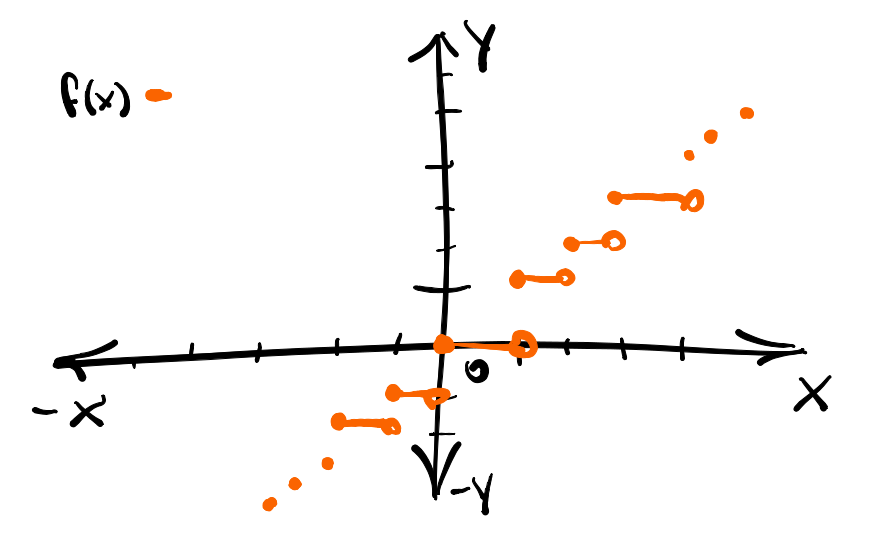
\includegraphics[scale=0.30]{escalerafn.png}
\caption[Función máximo entero.]{Función máximo entero.  } \label{escalerafn}
\end{figure}
\end{center}

La imagen de la función es discreta, es decir, tomar ciertos valores y no es un \textit{continuo} de valores. 
\newpage
\subsection{Dominio de una función por partes}

Al momento de analizar el dominio completo de la función por partes, se debe ver la definición de la misma. Si se ve el lado derecho, se encuentran las expresiones de las funciones y al lado izquierdo los intervalos en los cuales se defines las funciones, justamente son el dominio de cada función. Entonces, el dominio de la función por partes es la unión de cada uno de los dominios de la funciones que lo conforman.\\

\begin{myexample}
Encontrar el dominio de siguiente función por partes:
\begin{eqnarray*}
 f(x)= \left\{\begin{array}{ll}
f_{1}(x)&, x< 0\\
f_{2}(x) &, x=0\\ 
f_{3}(x) &, x>0 \\
\end{array} \hspace{6px} \right.
\end{eqnarray*}
$Dom(f(x))=Dom(f_{1}(x))\cup Dom(f_{2}(x))\cup Dom(f_{3}(x))=\mathbb{R}$
\end{myexample}
En el ejemplo anterior se ve que el dominio son todos los números reales, ya que entre los tres dominios completan el intervalo $]-\infty,\infty[$. En el caso en que algún punto o intervalo no sea considerado aparecen los tramos en que la función no está definida.

\begin{myexample}
Encontrar el dominio de siguiente función por partes:
\begin{eqnarray*}
 g(x)= \left\{\begin{array}{ll}
g_{1}(x)&, -5<x<1\\
g_{2}(x) &, 1\leq x\leq 10\\ 
g_{3}(x) &, 15<x<20 \\
\end{array} \hspace{6px} \right.
\end{eqnarray*}

\begin{eqnarray*}
Dom(g(x))&=& Dom(g_{1}(x))\cup Dom(g_{2}(x))\cup Dom(g_{3}(x))\nonumber\\
&=&]-5,1[\cup [1,10]\cup ]15,20[\\
&=&]-5,10]\cup ]15,20[\\
\end{eqnarray*}
\end{myexample}
Para este caso se ve, en la definición y en el resultado del dominio, que la función tiene tramos no definidos. Específicamente, los intervalos $]-\infty,-5]$, $]10,15]$ y $[20,\infty[$ no son parte del dominio.

\section{Combinación de funciones}
Luego de ver las funciones por partes, sigue la opción de combinar funciones, que en estricto rigor ya lo hemos visto cuando sumamos, restamos o dividimos polinomios. Las operaciones formales que se pueden hacer al momento de combinar funciones son: \\
\begin{mydef}
\textbf{Combinación de funciones.} Sea $f(x)$ y $g(x)$ dos funciones definidas en los números reales, entonces las operaciones de suma ($+$), resta ($-$), división ($\slash$) y la multiplicación ($\cdot$) se define de la siguiente manera:\\

\noindent i) $(f+g)(x)=f(x)+g(x)$.\\
\noindent ii) $(f-g)(x)=f(x)-g(x)$.\\
\noindent iii) $(f\cdot g)(x)=f(x)\cdot g(x)$.\\
\noindent iv) $\left(\dfrac{f}{g} \right)(x)=\dfrac{f(x)}{g(x)}$, siempre que $g(x)\neq 0$.\\
\end{mydef}

\begin{myexample}
Escribir la función resultante de las cuatro operaciones con las funciones $f(x)=x^{2}-1$ y $g(x)=x+1$:\\

\noindent i)$f(x)+g(x)=x^{2}+x$.\\
\noindent ii) $f(x)-g(x)=x^{2}-x-2$.\\
\noindent iii) $f(x)\cdot g(x)=(x^{2}-1)(x+1)=x^{2}(x+1)-(x+1)=x^{3}+x^{2}-x-1$.\\
\noindent iv) $\dfrac{f(x)}{g(x)}=\dfrac{x^{2}-1}{x+1}=\dfrac{(x+1)(x-1)}{x+1}=x-1$.\\
\end{myexample}

\subsection{Dominio de una función combinada}
Es importante que por más combinaciones que se hagan entre dos o más funciones sigan estando definidas en los números reales, suena obvio, pero hay verificarlo. El dominio que tiene una función combinada es el conjunto más grande que tiene en común todas las funciones, entonces es la intersección del dominio de las funciones. Para el caso de la división se suma la condición que la expresión del denominador debe ser diferente de cero.\\
 Supongamos el ejemplo que tenemos dos funciones $f_{1}(x)$ y $f_{2}(x)$ con su conjunto dominio $X_{1}$ y $X_{2}$ respectivamente. Entonces, el dominio de la función combinada es: \\
 
 \noindent i) El dominio para las operaciones de suma, resta y y multiplicación es $X_{1}\cap X_{2}$.\\
 
  \noindent ii) El dominio para las operacion de división es $\{x|x\in  X_{1}\cap X_{2}, g(x)\neq 0\}$.\\
  
\begin{myexample}
Sea $f(x)=\sqrt{x-3}$ y $g(x)=\sqrt{x+4}$ dos funciones definidas en los números reales, calcule el dominio de la función combinada $f(x)/g(x)$.\\

\textit{Sol:} Primero sabemos que las funciones de raíz cuadrada estén definidas en los números reales y deben ser mayor o igual que cero ($\geq 0$). Además, la función del denominador debe cumplir que $g(x)\neq 0$.\\
%Agregar definición con cuantificadores
\begin{eqnarray*}
h(x)=\dfrac{f(x)}{g(x)}&=&\dfrac{\sqrt{x-3}}{\sqrt{x+4}}\\
Dom(f(x))&\cap &Dom(g(x)), g(x)\neq 0\\
x-3\geq 0 &\cap &x+4>0\\
x\geq +3 &\cap &x>-4 \\
\left[3,+\infty \right] &\cap & \left]-4,+\infty \right[\\
Dom\left(\dfrac{f(x)}{g(x)} \right) &=&\left[3,+\infty \right] 
\end{eqnarray*}
Notar que la condición del denominador sea diferente de cero se cumplió al pasar de $\geq$ a $>$.
\end{myexample}

\section{Composición de funciones}
Al principio de esta sección se mencionó que dentro del paréntesis de la función ($f()$) va la incógnita, por ende lo que se reemplaza en este caso es la función $f()$. En esta sección veremos que ocurre cuando dentro de la función hay otra función, como por ejemplo $f(g(x))$.\\

\begin{mydef}
\textbf{Composición de funciones.} Sea $f(x)$ y $g(x)$ dos funciones definidas en los números reales. La composición de ambas funciones se escribe de la siguiente manera:\\
\begin{eqnarray*}
(f\circ g)(x)&=& f(g(x)) \\
(g\circ f)(x)&=&g(f(x)) \\
\end{eqnarray*}
\end{mydef}

\begin{myexample}
Sea $f(x)=x^{2} +x$ y $g(x)=x+5$ dos funciones definidas en los números reales, calcular las funciones compuestas $f(g(x))$ y $g(f(x))$.\\
\begin{eqnarray*}
f(g(x))&=& f(x+5)= (g(x))^{2}+(g(x))=(x+5)^{2}+(x+5)\\
&=& x^{2}+10x+25+x+5\\
&=&x^{2}+11x+30.
\end{eqnarray*}
\begin{eqnarray*}
g(f(x))&=& g(x^{2}+x)=g(x)+5=x^{2}+x+5 \\
\end{eqnarray*}
\end{myexample}


\subsection{Dominio de una función compuesta}
El dominio de la función compuesta es el conjunto formado por los números que están en el dominio de $g(x)$, tales que $g(x)$ esté en el dominio de $f(x)$. En otras palabras, son los números que están en g(x) y que además no indeterminan $f(x)$. La definición del dominio de una función compuesta por $f(x)$ y $g(x)$ es:
\begin{eqnarray}
Dom\left(f(g(x)) \right)=\{x\in Dom(g(x))\wedge g(x)\in Dom(f(x))\}\\
Dom\left(g(f(x)) \right)=\{x\in Dom(f(x))\wedge f(x)\in Dom(g(x))\}
\end{eqnarray}

\begin{myexample}
Sea $f(x)=x/(x+2)$ y $g(x)=1/(x-1)$ dos funciones definidas en los números reales. Calcular el dominio de la función compuesta $f(g(x))$.

\begin{eqnarray*}
Dom(f(g(x)))&=& x\in Dom(g(x)) \wedge g(x)\in Dom(f(x))\\
&=& x\neq 1 \wedge \dfrac{1}{x-1}\neq -2\\
&=& x\neq 1 \wedge x\neq\dfrac{1}{2}\\
&=& \mathbb{R}-\{1\} \cap \mathbb{R}-\biggl\{\dfrac{1}{2}\biggl\}\\
&=&\mathbb{R}-\biggl\{ 1,\dfrac{1}{2}\biggl\}
\end{eqnarray*}
\end{myexample}

\begin{myexample}
Sea $f(x)=\sqrt{x}$ y $g(x)=x-2$. Calcular el dominio de $f(g(x))$:\\
\begin{eqnarray*}
Dom(f(g(x)))&=& Dom(f(x-2))\\
&=& Dom(\sqrt{x-2})\\
&=& \sqrt{x-2}\\
&=& x-2\geq 0\\
&=& x\geq 2\\
Dom(f(g(x)))&=& [2,+\infty [ \\
\end{eqnarray*}
\end{myexample}

\section{Cociente de diferencias}
\label{cuociente0}
Ahora, veremos una aplicación de la composición de funciones. Suponga que tomamos dos puntos del gráfico de una función ¿Cuán cerca están estos puntos? Tanto como uno quiera. Definiremos la distancia entre los dos puntos con la variable $h$, que repito, es muy pero muy pequeña. \\ Al conocer dos puntos de una función se abre el abanico de opciones para calcular. Una de ellas es trazar una recta entre los puntos y calcular la pendiente de dicha recta. Recordando la fórmula de la pendiente de una recta:\\ 

\begin{eqnarray}
m = \dfrac{y_{2}-y_{1}}{x_{2}-x_{1}}
\end{eqnarray}
Donde $x_{i}$ y $y_{i}$ son los valores de dos puntos $(x_{1},y_{2})$ y $(x_{2},y_{2})$ en un plano cartesiano. Si hacemos lo mismo pero ahora los puntos son $(x,f(x))$ y $(x+h,f(x+h))$, la pendiente es:\\
\begin{eqnarray}
m&=&\dfrac{f(x+h)-f(x)}{(x+h)-x}\nonumber \\
m&=&\dfrac{f(x+h)-f(x)}{h}
\label{dif}
\end{eqnarray} 
La ecuación (\ref{dif}) es el primer acercamiento al cálculo infinitesimal, donde la variable $h$ además de ser pequeño representa el \textit{cambio} que sufre la función.

\begin{myexample}
Calcular el cociente de diferencias de $f(x)=x^{2}+2$.\\

\noindent Sol: Primero se debe calcular la función compuesta $f(x+h)$.
\begin{eqnarray*}
f(x+h)&=&(x+h)^{2}+2 \\
&=&x^{2}+2xh+h^{2}+2\\
\end{eqnarray*}
Ahora, reemplazamos en la ecuación (\ref{dif}):
\begin{eqnarray*}
m&=&\dfrac{f(x+h)-f(x)}{h}\\
&=&\dfrac{x^{2}+2xh+h^{2}+2-(x^{2}+2)}{h}\\
&=&\dfrac{2xh+h^{2}}{h}\\
&=&\dfrac{h(2x+h)}{h}\\
&=&2x+h,\hspace*{15px} h\approx 0\\
&=&2x \\
\end{eqnarray*}
Entonces el cocientes de diferencias de $f(x)$ es $2x$, más adelante veremos que este cociente es la \textbf{derivada} de $f(x)$ y se puede denotar como $f'(x)$.
\end{myexample}

\begin{center}
\begin{figure}[h!]
\centering
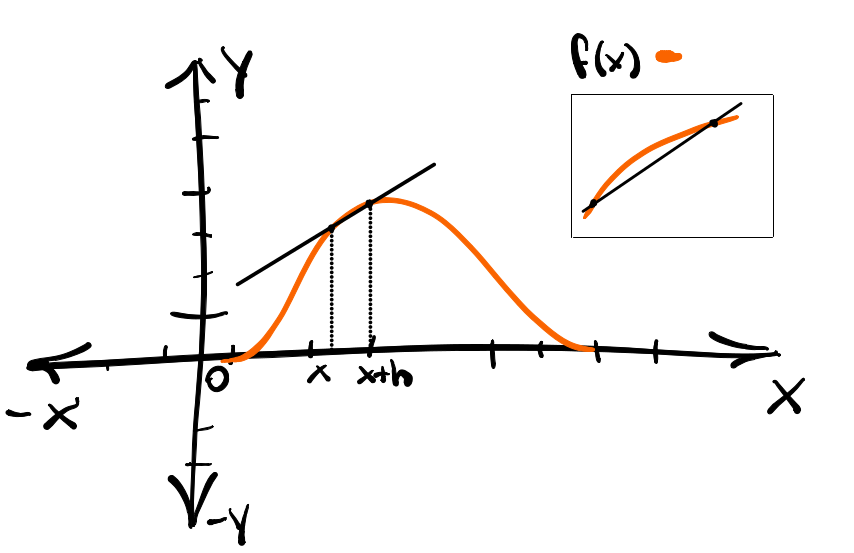
\includegraphics[scale=0.35]{cocientefn.png}
\caption[Cociente de diferencia.]{Cociente de diferencia. La línea naranja continua representa la función, la línea negra continua representa la recta de los puntos y las líneas punteadas muestran la diferencia entre los puntos (la distancia es representada por $h$). El gráfico insertado amplía la función y la recta, donde para los dos puntos hay una distancia $h$.} \label{cocifn}
\end{figure}
\end{center}
\section{Funciones inversas}
En un principio, vimos en (\ref{fn00}) que las funciones son una correspondencia entre un dominio $X$ y una imagen $Y$. Siempre a un elemento $x_{i}$ del dominio se le asocia un elemento $y_{i}$ de la imagen y por más que haya casos en que hay más de un elemento del dominio para un mismo $y_{i}$ (por ejemplo las funciones del tipo $x^{2}$), las funciones que por cada elemento del dominio tienen un solo elemento de la imagen se llaman funciones uno a uno.

\begin{mydef}
\textbf{Función uno a uno.} Sea una función $f(x)$ definida en los números reales, es uno a uno o biunívoca si cada número en el rango de $f(x)$ está asociado con exactamente con \textbf{un} número en su dominio $X$.  
\end{mydef}

La forma \textit{gráfica} de ver si una función es uno a uno es trazar una línea horizontalmente, si la línea toca dos puntos, entonces no es una función biunívoca, en caso contrario si lo es.\\
Al momento definir este tipo de funciones, se puede hacer en función de los elementos de dominio.

\begin{mydef}
\textbf{Función uno a uno.} Una función es uno a uno si y solo si $f(x_{1})=f(x_{2})$ implica que $x_{1}=x_{2}$ para toda $x_{1}$ y $x_{2}$ en el dominio de f.
\end{mydef}

%%%%%
\begin{center}
\begin{figure}[h!]
\centering
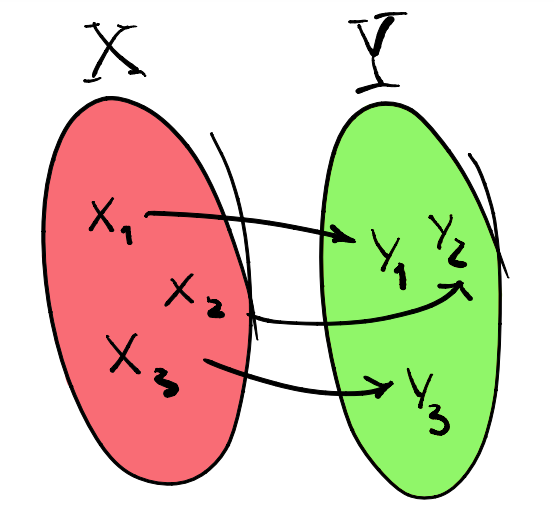
\includegraphics[scale=0.4]{unoaunofn.png}
\caption[Función uno a uno.]{Función uno a uno. Los óvalos rojos y verde representan el dominio e imagen de la función $f(x)$. Las flechas muestran que cada elemento $x_{i}$ $(i=1,2,3)$ del dominio tiene un elemento $y_{i}$ $(i=1,2,3)$ de la imagen.} \label{unafn}
\end{figure}
\end{center}
\begin{myexample}
Sea $f(x)=x+1$, comprobar si es una función uno a uno.
\begin{eqnarray*}
x_{1}+1&=&x_{2}+1 \hspace{10px} \slash -1 \\
x_{1}&=&x_{2}
\end{eqnarray*}
Como $x_{1}=x_{2}$ implica que $f(x_{1})=f(x_{2})$, por lo tanto $f(x)$ es una función uno a uno.
\end{myexample}

\begin{myexample}
Sea $f(x)=x^{2}+1$, comprobar si es una función uno a uno.

\begin{eqnarray*}
x_{1}^{2}+1&=&x_{2}^{2}+1 \hspace{10px} \slash -1 \\
x_{1}^{2}&=&x_{2}^{2}  \hspace{10px} \slash \sqrt{•}\\
\sqrt{x_{1}^{2}}&=&\sqrt{x_{2}^{2}}\\
|x_{1}|&=&|x_{2}|\\
\end{eqnarray*}
Como ambos $x_{i}$ están con valor absoluto, puede dar el caso de que $x_{1}=-x_{2}$ o $-x_{1}=x_{2}$, por lo tanto no se cumplen las condiciones de una función biunívoca. Entonces, como $x_{1}\neq x_{2}$ implica que $f(x_{1})\neq f(x_{2})$ y $f(x)$ no es una función uno a uno.
\end{myexample}

Si imaginamos que el tomar un elemento $x_{1}$ del dominio $X$ de la función $f(x)$ es un \textit{camino de ida} y que además esta función es uno a uno, podemos hacer el \textit{camino de vuelta} para pasar de un elemento de la imagen $y_{i}$ al elemento del dominio $x_{i}$. Esto implica aplicar una función (desconocida hasta el momento) que pase los elementos de la imagen al dominio de la función, esa función se llama función inversa.

\begin{mydef}
\textbf{Función inversa.} Sea f(x) una función uno a uno, con dominio $X$ e Imagen $Y$. La inversa de f(x) es la función denotada por $f^{-1}$, cuyo dominio es $Y$ e imagen $X$.

\noindent i) $f(f^{-1}(x))=x$ para toda $x$ en $Y$.\\
\noindent ii) $f^{-1}(f(x))=y$ para toda $y$ en $X$.\\
\end{mydef}

\begin{mydef}
\textbf{Propiedades de las funciones inversas.} Sea $f(x)$ una función en los números reales.\\

\noindent i) $Dom(f^{-1}(x))=Img(f(x))$. \\

\noindent ii) $Dom(f(x))=Img(f^{-1}(x))$. \\

\noindent iii) $y=f(x)$ equivale a $x=f^{-1}(y)$. \\

\noindent iv) La función inversa $f^{-1}$ es uno a uno. \\

\noindent v) La función inversa de $f(x)$ es $f^{-1}(x)$, entonces $f^{-1}(f^{-1}(x))=f(x)$ . \\

\noindent vi) La inversa de $f(x)$ es única. \\
\label{propinv}
\end{mydef}

\begin{center}
\begin{figure}[h!]
\centering
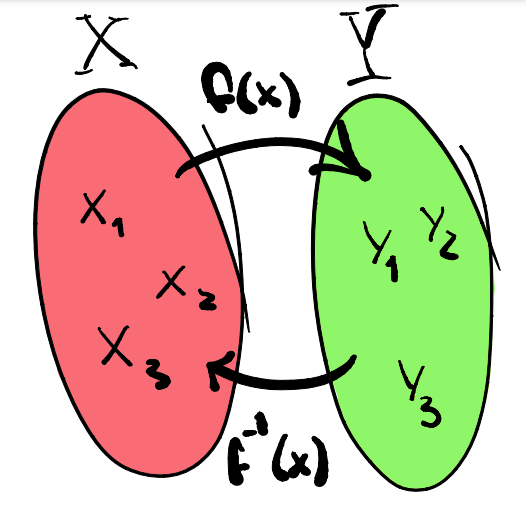
\includegraphics[scale=0.4]{inversafn.png}
\caption[Función inversa.]{Función inversa. Las flechas negras muestran que la función $f(x)$ va desde el dominio a la imagen y $f^{-1}$ va desde la imagen al dominio.} \label{inversafn}
\end{figure}
\end{center}

\begin{myexample}
Sea $f(x)=$, determinar la función inversa de $f(x)$. \\

\noindent Sol: En términos generales, se cambian los $'x'$ de la expresión por $f^{-1}(x)$ o por $'y'$ y luego se despeja dicha variable cambiada.\\
\begin{eqnarray*}
f(x)&=&\sqrt{x+3} \\
y=\sqrt{x+3}& \longrightarrow &x=\sqrt{y+3} \\
x&=&\sqrt{y+3}\\
x^{2}&=&y+3 \\
x^{2}-3 &=&y \hspace*{8px}\longleftarrow inversa\\
\end{eqnarray*}
El $Dom(f^{-1}(x))$ son todos los números reales, que a su vez es la imagen de $f(x)$.
\end{myexample}

\subsection{Gráficas de la función inversa}
En las propiedades vistas en las definiciones (\ref{propinv}) y en la figura (\ref{inversafn}) se ve que la función y su inversa son \textit{opuestas}. En términos gráficos, si los puntos $(x_{i},y_{i})$ del plano pertenecen a la función $f(x)$, los puntos de la inversa $f^{-1}(x)$ son ($y_{i},x_{i}$). Esto es que la representación de la función inversa  es una reflexión de la función original. \\
 


\begin{center}
\begin{figure}[h!]
\centering
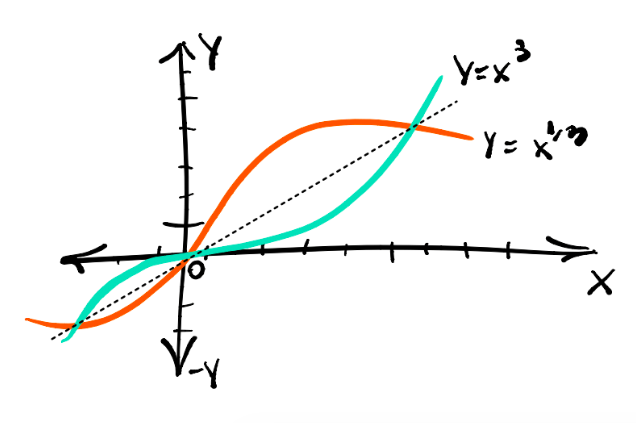
\includegraphics[scale=0.4]{invergrfn.png}
\caption[Grafico de una función inversa.]{Grafico de una función inversa. La función inversa es la reflexión con respecto al eje de simetría (representado por la linea negra punteada).} \label{Graficofnin}
\end{figure}
\end{center}

%\section{Problemas con enunciado}
%En esta sección juntaremos los conceptos para acercarlos a problemas con enunciado. Usualmente, como veremos ahora y durante este curso en general son situaciones ideales, es decir, no consideramos todas variables o son situaciones ficticias para ejercitar los tópicos. 
%
%%inversa,cociente de diferencia, fn combinadas, función escalón,interseccion con los ejes, transformaciones y deformaciones, funcion par e impar
%Resolver los siguientes problemas:\\
%
%\noindent 1) El consumo de mascarillas en el año 2016 tuvo la forma $5x+60$ y en el 2020 fue $10x-90$. Si $x$ representa los días del año ($x=1,2,3,...,365$), responda las siguientes preguntas:\\
%
%\noindent 1.a) ¿ Qué función cruza el eje $y$ en su parte positiva?
%\noindent \textit{Sol:} $f(x)=5x+60$ \\
%
%\noindent 1.b) ¿ Qué función cruza el eje $x$ en su parte positiva? 
%\noindent \textit{Sol:} $f(x)=10x-90$\\
%
%\noindent 1.c) ¿ En que año se utilizaron más mascarillas en diciembre?\\
%\noindent \textit{Sol:} Una pista se puede deducir por la pendiente de la función del año 2020, que es mayor, entonces ese es el año de mayor uso en diciembre. Lo segundo es reemplazar un número de $x$ que equivaldría a estar en diciembre \\
%\begin{eqnarray*}
%5x+60 \hspace{8px} &vs& \hspace{8px} 10x-90 \\
%5(360)+60 \hspace{8px} &vs& \hspace{8px} 10(360)-90 \\
%1860 \hspace{8px} &< & \hspace{8px} 3510 
%\end{eqnarray*}
%Se concluye que en el año 2020 se utilizaron mas mascarillas.\\
%
%\noindent 1.d) ¿ En que día del año se ocuparon el mismo número de mascarillas?
%
%\noindent \textit{Sol:} Si se ocuparon el mismo número, nos dice que ambas rectas tuvieron la misma imagen (número de mascarillas). Entonces, se deben interceptar ambas ecuaciones lineales. \\
%\begin{eqnarray*}
%5x+60  &=&  10x-90 \\
%90+60  &=&  10x-5x\\
%150  &=&  5x\\
%x  &=&  30
%\end{eqnarray*}
%
%\begin{center}
%\begin{figure}[h!]
%\centering
%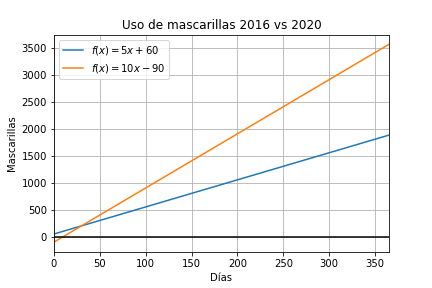
\includegraphics[scale=0.8]{mascarillas.png}
%\caption{Gráfica de las rectas del problema 1.} \label{prob1}
%\end{figure}
%\end{center}

\section{Funciones polinomiales}
En la sección (\ref{fnlincua}) se vio desde la función constante ($ax^{0}$) hasta la función cuadrática ($ax^{2}$), pero este tipo de funciones son parte de un conjunto más grande, las polinomiales. Ahora entraremos en detalles de como graficar este tipo de funciones. Recordar la ecuación (\ref{polfn}), donde el exponente es un número entero no negativo y en caso de que $n$ no cumpla estas condiciones, la función no es polinomial (Ejemplo: $x^{-1}$ o $x^{1/2}$).

Cuando hablamos de la función cuadrática tenemos en mente el $x^{2}$, de la misma manera pasa con el cúbico y su representación $x^{3}$. Cuando el exponente es mayor se le llama $n-$ésimo considerando el exponente mayor como nombre del polinomio (Ejemplo: $x^{8}+4$ polinomio de octavo orden). 

\begin{mydef}
\textbf{Funciones polinomiales.} Sea $f(x)$ una función polinomial definida en los números reales, se desprenden los siguientes casos:\\

\noindent i) Si $f(x)=a_{0}$ es una función polinomial constante.\\
\noindent ii) Si $f(x)=a_{1}x+a_{0}$ es una función polinomial lineal.\\
\noindent iii) Si $f(x)=a_{2}x^{2}+a_{1}x+a_{0}$ es una función polinomial cuadrática.\\
\noindent iv) Si $f(x)=a_{3}x^{3}+a_{2}x^{2}+a_{1}x+a_{0}$ es una función polinomial cúbica.\\
\noindent v) Si $f(x)=a_{n}x^{n}+a_{n-1}x^{n-1}+\cdots+a_{0}x^{0}$ es una función polinomial $n-$ésima.
\end{mydef}

En (\ref{linfn}) y (\ref{cuadfn}) se muestra la gráfica de las funciones lineales y cuadrática respectivamente, pero es más difícil a simple vista dilucidar las gráficas de órdenes mayores. Por lo mismo, hay que tener en consideración conceptos anteriores como traslaciones, deformaciones, simetrías o intersecciones con los ejes. \\

Lo más simple es partir por el caso en que la función es un solo término de la forma $x^{n}$, aquí se puede tener el caso en que $n$ es par o impar. \\

\begin{center}
\begin{figure}[h!]
\centering
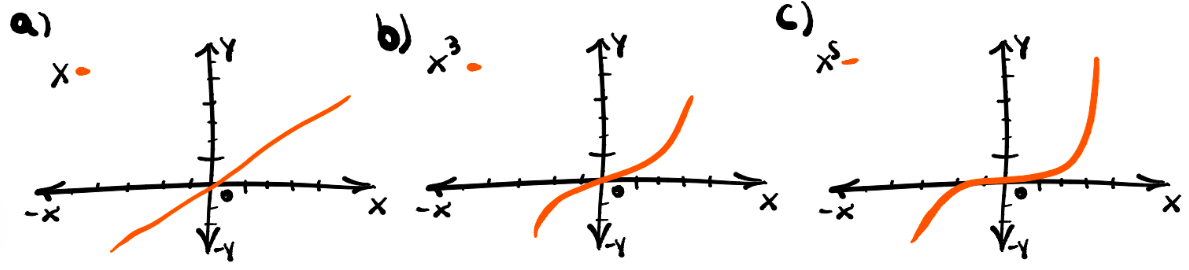
\includegraphics[scale=0.5]{fnimpares.png}
\caption[Ejemplo funciones impares.]{Ejemplo funciones impares. a) Es la función lineal y en los casos b) y c) se ve como se va aplanando la región que pasa por el origen del plano a medida que aumenta el $n$ de $x^{n}$.} \label{fnimp}
\end{figure}
\end{center}
 
 \begin{center}
\begin{figure}[h!]
\centering
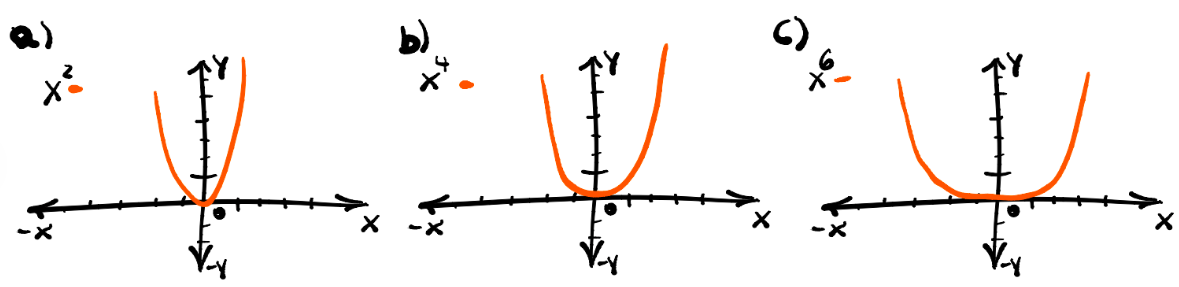
\includegraphics[scale=0.52]{fnpares.png}
\caption[Ejemplo funciones pares.]{Ejemplo funciones pares. a) Es la función cuadrática y en los casos b) y c) se ve como se va aplanando la región que pasa por el origen del plano, al igual que en el caso de los exponentes impares.} \label{fnpar}
\end{figure}
\end{center}

A estas funciones se debe sumar las variantes de las traslaciones, si se suma o resta una constante dentro o fuera del término principal, $x^{n}\pm c$ o $(x\pm c)^{n}+d$. \\
Por el momento, entraremos solo en el caso $x^{n}$ y debemos descifrar su comportamiento. En las figuras (\ref{fnimp}) y (\ref{fnpar}) se muestran todas las funciones cuando pasan por el origen, es decir, que los valores que toman los $x_{i}$ son muy bajos, pero ¿Qué ocurre cuando $x$ es muy grande? Lo que nos dirá esta respuesta es como se comporta la función muy lejos del origen.\\
El tomar valores altos del dominio de la función, es decir, que $x\longrightarrow +\infty$ o $x\longrightarrow -\infty$ hace ver como se comporta la función en \textbf{los extremos}.

\begin{mydef}
\label{extrefn0}
\textbf{Comportamiento de los extremos.} Cuando $x\longrightarrow\pm\infty$ la gráfica de una función polinomial\footnote{El símbolo $\rightarrow$ significa `tiende'. Es ponerse en caso en que la variable toma valores muy grandes.}
\begin{eqnarray*}
f(x)&=&a_{n}x^{n}+a_{n-1}x^{n-1}+a_{n-2}x^{n-2}+\cdots +a_{0} \\
\end{eqnarray*}
se asemeja a la gráfica $f(x)=a_{n}x^{n}$. Esto se debe a que los términos que le siguen aportan muy poco a la gráfica, en consecuencia la alteran muy poco.
\end{mydef}

\begin{myexample}
Sea $f(x)=7x^{3}+5x-20$, mostrar a que gráfica se asemeja esta función.
\begin{eqnarray*}
f(x)&=& 7x^{3}+5x-20 \\
f(x)&=& x^{3}\left(7+\dfrac{5x}{x^{3}}-\dfrac{20}{x^{3}} \right)\\
f(x)&=& x^{3}\left(7+\dfrac{5}{x^{2}} -\dfrac{20}{x^{3}}\right) \hspace{8px} x\longrightarrow \pm\infty\\
f(x)&=& 7x^{3}
\end{eqnarray*}
\end{myexample}
Visto el ejemplo anterior, se puede tener cuatro posibilidades en los extremos y dependen si el exponente es par o impar. Si consideramos el polinomio de la forma definida en (\ref{extrefn0}) y usando la aproximación del coeficiente principal obtenemos la siguiente información de la función polinomial.
\begin{table}[h!]
\begin{center}
		\begin{tabular}{|c|c|c|}
		\hline
		& $a_{n}<0$ & $a_{n}>0$ \\ 
		\hline
		Exponente par & $f(x<0)\longrightarrow -\infty$, $f(x>0)\longrightarrow -\infty$ &  $f(x<0)\longrightarrow \infty$, $f(x>0)\longrightarrow \infty$ \\
		\hline
		Exponente impar & $f(x<0)\longrightarrow \infty$, $f(x>0)\longrightarrow -\infty$ &  $f(x<0)\longrightarrow -\infty$, $f(x>0)\longrightarrow \infty$ \\
		\hline
		\end{tabular}
		\caption[Tabla de los extremos de una función polinomial.]{Tabla de los extremos de una función polinomial.}
\end{center}
\end{table}


\section{Funciones racionales}
\label{funrac0}
%300
Al igual que los números, los polinomios tienen sus operaciones y forman nuevas funciones, para el caso de la división son las funciones racionales. \\

\begin{mydef}
\textbf{Función racional. }Una función racional $y=f(x)$ es una función que tiene la forma:
\begin{eqnarray}
f(x)=\dfrac{P(x)}{Q(x)}
\end{eqnarray}
en donde $P(x)$ y $Q(x)$ son funciones polinomiales. Además, el denominador debe seer distinto de cero, $Q(x)\neq 0$.
\end{mydef}

Al momento de graficar las funciones racionales no es tan trivial, por lo que hay que sumar herramientas a las ya conocidas (Simetrías, intersecciones con los ejes, desplazamiento, etc.) para modelar las funciones, es por ellos que entraremos en detalle con las \textit{asíntotas}.\\

Una asíntota es una función lineal (una recta) que se aproxima de forma continua a la gráfica de una función $f(x)$, en otras palabras, la función $f(x)$ tiende al valor de la asíntota. La notación que introduciremos cuando $x$ se aproxima a un número $a$ o tiende a $\pm\infty$ es la siguiente:
\begin{itemize}
	\item $x\rightarrow a^{-}$, la variable $x$ tiende a $a$ desde la izquierda, es decir, a través de números más pequeños que $a$.\\
	\item $x\rightarrow a^{+}$, la variable $x$ tiende a $a$ desde la derecha, es decir, a través de números más grandes que $a$.\\
	\item $x\rightarrow a$, la variable $x$ tiende a $a$ desde la derecha y la izquierda.\\
	\item $x\rightarrow -\infty$, la variable $x$ tiende a $-\infty$, es decir, se vuelve no acotado en dirección negativa.\\
	\item $x\rightarrow \infty$, la variable $x$ tiende a $\infty$, es decir, se vuelve no acotado en dirección positiva.\\
\end{itemize}

\subsection{Asíntotas verticales}
Ocuparemos la notación introducida para definir los casos de asíntotas. Aquí veremos dos casos, horizontales y verticales. Como su nombre lo dice, las asíntotas verticales es una línea vertical que cruza por el eje $x$ y que nunca toca a la gráfica.

\begin{mydef}
\label{asintvert}
\textbf{Asíntotas verticales. } Se dice que una recta $x=a$ es una asíntota vertical de la gráfica de una función $f(x)$, si se cumple al menos una de estas seis condiciones:
\begin{itemize}
	\item $f(x)\rightarrow -\infty$ cuando $x\rightarrow a^{-}$ \\
	\item $f(x)\rightarrow -\infty$ cuando $x\rightarrow a^{+}$ \\
	\item $f(x)\rightarrow -\infty$ cuando $x\rightarrow a$ \\
	\item $f(x)\rightarrow +\infty$ cuando $x\rightarrow a^{-}$ \\
	\item $f(x)\rightarrow +\infty$ cuando $x\rightarrow a^{+}$ \\
	\item $f(x)\rightarrow +\infty$ cuando $x\rightarrow a$ \\
\end{itemize}
\end{mydef}

La definición (\ref{asintvert}) explica que cuando uno se acerca a las asíntotas, se puede hacer por la izquierda o por la derecha. Luego de acercarse por ambos lados puede darse el caso en que coincidan, entonces nace el concepto de una \textit{función continua} en el punto que uno se acerca. Si la función tiene una asíntota es una función discontinua, en palabras simples, es una función continua si puedo dibujar la gráfica sin levantar el lápiz.

 \begin{center}
\begin{figure}[h!]
\centering
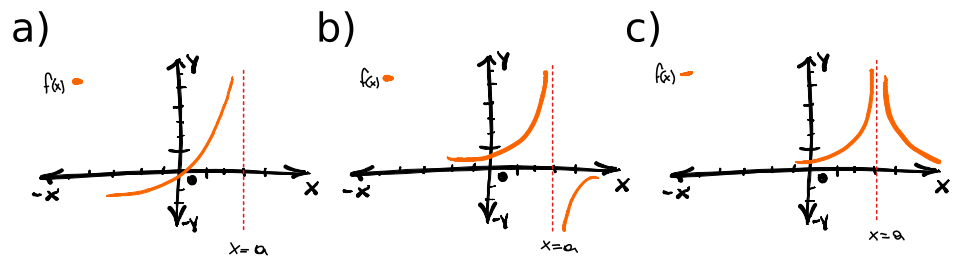
\includegraphics[scale=0.6]{asintvert.png}
\caption[Asíntotas verticales.]{Asíntotas verticales. a) Se ve en la gráfica que cuando me acerco por la izquierda la función tiende a $+\infty$, es decir, que $f(x)\rightarrow +\infty$ cuando $x\rightarrow a^{-}$.  b) $f(x)\rightarrow +\infty$ cuando $x\rightarrow a^{-}$ y $f(x)\rightarrow -\infty$ cuando $x\rightarrow a^{+}$. c) $f(x)\rightarrow \infty$ cuando $x\rightarrow a$. } \label{asintvert0}
\end{figure}
\end{center}

Ahora, ¿Las funciones de la figura (\ref{asintvert0}) son continuas?. La respuesta es si y no ¿Como?, si uno analiza la función completa claro que no es continua, porque tiene una asíntota de por medio, pero si uno toma un solo tramo (por ejemplo los casos b y c) de las funciones si lo son. Entonces la conclusión es que la función $f(x)$ es continua o discontinua según el tramo que se analice.

\subsubsection{Determinación de asíntotas verticales}

Para determinar las asíntotas se debe analizar la función racional de formar general
\begin{eqnarray}
\dfrac{P(x)}{Q(x)}=\dfrac{a_{n}x^{n}+a_{n-1}x^{x-1}+\cdots +a_{1}x+a_{0}}{b_{m}x^{m}+b_{m-1}x^{m-1}+\cdots + b_{1}x+b_{0}}
\label{fracpol}
\end{eqnarray}

Ahora supongamos que los polinomios $P(x)$ y $Q(x)$ de la ecuación (\ref{fracpol}) no tienen factores comunes (que no se pueden simplificar más). En este caso: \\

\textit{Si a es un número real tal que Q(a)=0, la recta x=a es una asíntota vertical de la gráfica de f(x).}\\

Entonces las soluciones de la ecuación del polinomio $Q(x)$ son las asíntotas verticales. Como el polinomio $Q(x)$ puede tener hasta $m$ raíces reales, entonces la gráfica puede tener hasta $m$ asíntotas verticales 
\begin{myexample}
Sea $f(x)$ una función definida en los números reales. Encontrar las asíntotas verticales de $f(x)$.
\begin{eqnarray*}
f(x)=\dfrac{P(x)}{Q(x)}&=&\dfrac{x^{2}+2}{x-2} \\
&=& x-2=0\\
x &=& 2
\end{eqnarray*}
$f(x)$ tiene una asíntota en $x=2$.

 \begin{center}
\begin{figure}[h!]
\centering
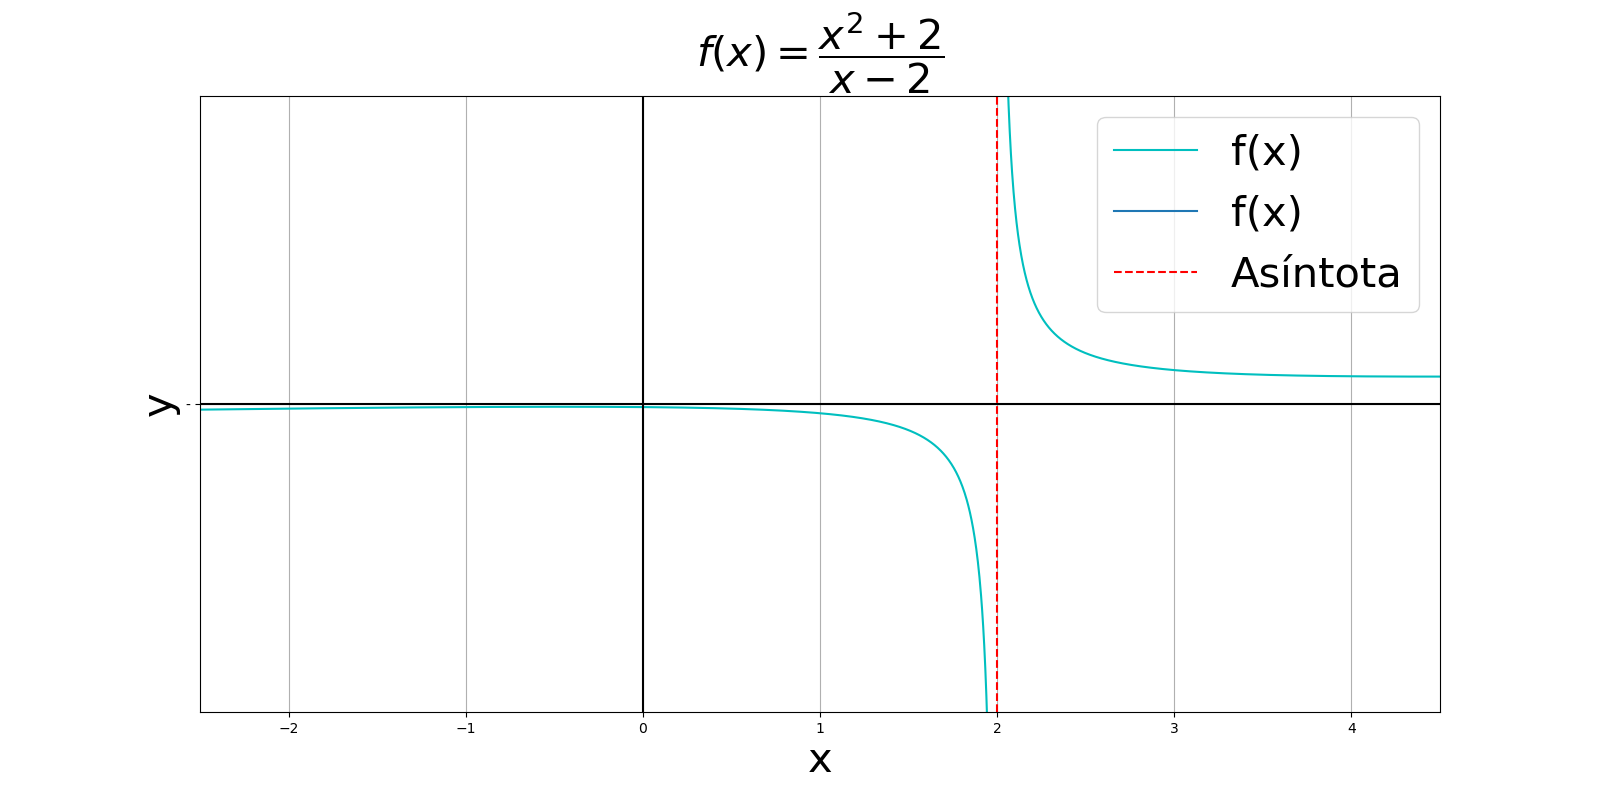
\includegraphics[scale=0.30]{asintver.png}
\caption{Gráfica de la función $f(x)$ con su asíntota en $x=2$.} \label{asintvert1}
\end{figure}
\end{center}
\end{myexample}

\subsection{Asíntotas horizontales}
Al igual que el caso vertical, existen asíntotas horizontales, pero ahora es una recta de valor constante. En este tipo de asíntotas muestran una diferencia con las verticales y es que se puede cruzar por la grafica.

\begin{mydef}
\textbf{Asíntotas horizontales. } Se dice que una recta $y=c$ es una asíntota horizontal de la gráfica de una función $f(x)$, si
\begin{itemize}
	\item $f(x)\rightarrow c$ cuando $x\rightarrow -\infty $ o si $f(x)\rightarrow c$ cuando $x\rightarrow +\infty $
\end{itemize}
\end{mydef}


\subsubsection{Determinación de asíntotas horizontales}
 Para el cálculo de las asíntotas horizontales se debe recurrir nuevamente al polinomio (\ref{fracpol}) con el detalle visto en la definición (\ref{extrefn0}). Recordando la definición, nos dice que a valores muy grandes de $x$ ($x\rightarrow \pm\infty$) la gráfica tiene la forma del término con el grado más alto del polinomio. Entonces, como los grados menores no aportan en los extremos, se reduce la expresión racional al primer termino del numerador y denominador. 

\begin{eqnarray}
f(x)&=&\dfrac{a_{n}x^{n}+a_{n-1}x^{x-1}+\cdots +a_{1}x+a_{0}}{b_{m}x^{m}+b_{m-1}x^{m-1}+\cdots + b_{1}x+b_{0}}\nonumber\\
&\approx &\dfrac{a_{n}x^{n}}{b_{m}x^{m}}\nonumber\\
&\approx & \dfrac{a_{n}}{b_{m}}x^{n-m}
\label{asinh0}
\end{eqnarray}

De la ecuación (\ref{asinh0}) se desprenden 3 casos:\\

\noindent a) Si $n=m$, $f(x)\approx \dfrac{a_{n}}{b_{m}}x^{n-m}\rightarrow \dfrac{a_{n}}{b_{m}}$ cuando $x\rightarrow \pm\infty$\\

\noindent b) Si $n<m$, $f(x)\approx \dfrac{a_{n}}{b_{m}}x^{n-m}= \dfrac{a_{n}}{b_{m}x^{n-m}}\rightarrow 0$ cuando $x\rightarrow \pm\infty$\\

\noindent c) Si $n>m$, $f(x)\approx \dfrac{a_{n}}{b_{m}}x^{n-m}= \dfrac{a_{n}x^{n-m}}{b_{m}}\rightarrow \infty$ cuando $x\rightarrow \pm\infty$\\

En resumen, el caso a) la asíntota es una recta horizontal donde $y= a_{n}/b_{m}$, el b) la asíntota es una recta $y=0$ y el caso c) no hay asíntota, pues diverge (se va a infinito) la función.
\begin{myexample}
Sea $f(x)$ una función definida en los números reales. Calcule la asíntota horizontal:
\begin{eqnarray*}
f(x)&=&\dfrac{8x}{x^{2}-2x+1}\\
&=&\dfrac{8x}{x^{2}\left(1-2\dfrac{1}{x}+\dfrac{1}{x^{2}}\right) }\\
&=&\dfrac{8x}{x^{2} }\\
&=&\dfrac{8}{x}, \hspace{10px} x\rightarrow \infty\\
y &=& 0 
\end{eqnarray*}

 \begin{center}
\begin{figure}[h!]
\centering
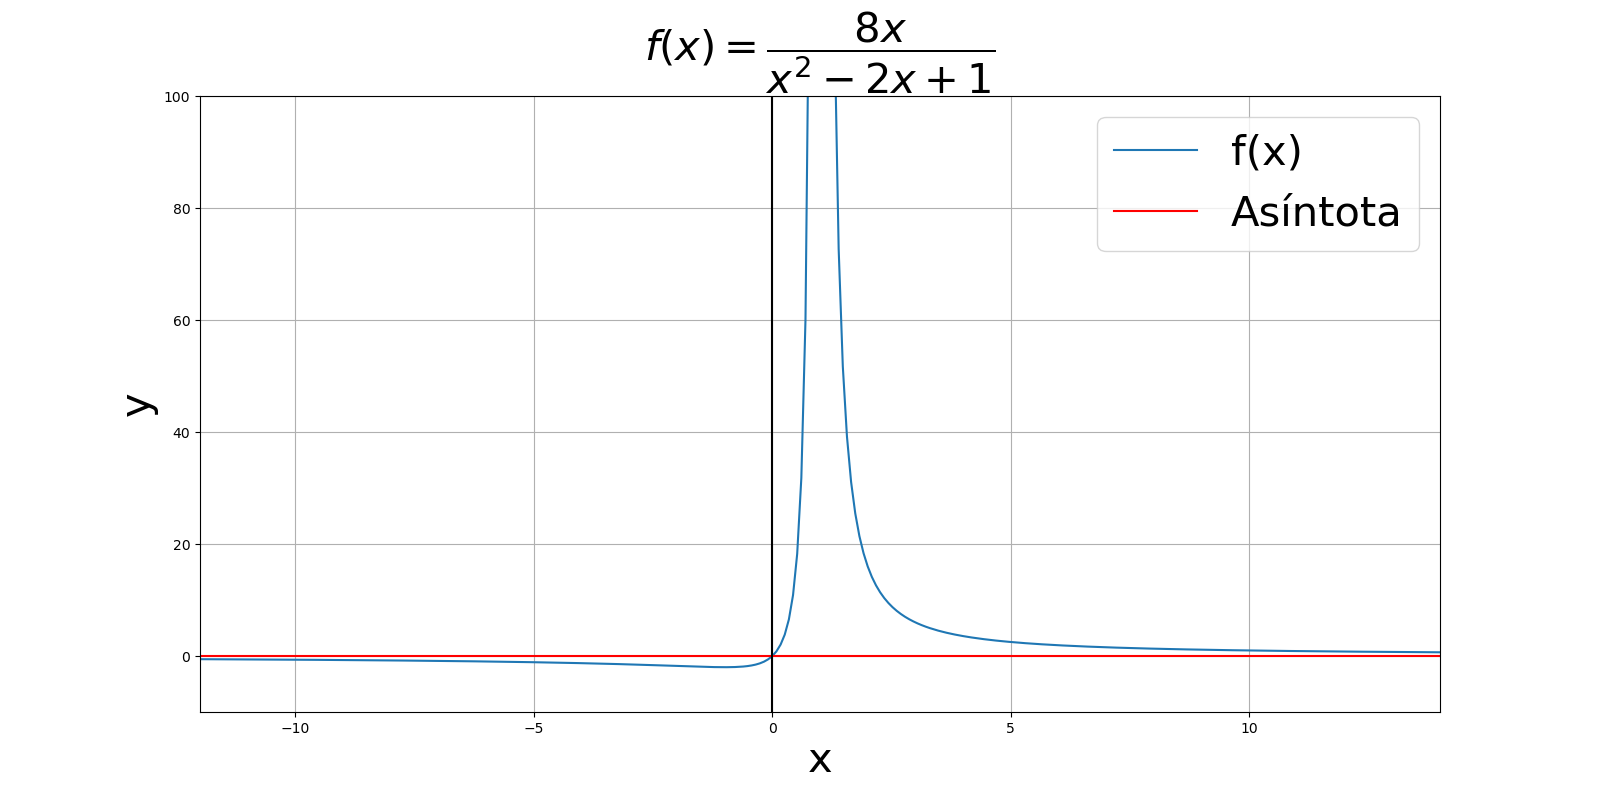
\includegraphics[scale=0.3]{asinth.png}
\caption[Gráfica de la función $f(x)$ con su asíntota horizontal en $y=0$.]{Gráfica de la función $f(x)$ con su asíntota horizontal en $y=0$. Notar que la función tiene una asíntota vertical, pero en este caso no es calculada.} \label{asintvert1}
\end{figure}
\end{center}
\end{myexample}
\newpage
\section{Funciones exponenciales}
En las secciones anteriores la variable es elevada a un número entero o decimal, para este caso veremos cuando un número es  elevado a la incógnita
\begin{mydef}
\textbf{Función exponencial.} Si $b>0$ y $b\neq 1$, una función exponencial $y=f(x)$ tiene la forma\\
\begin{eqnarray}
f(x)=b^{x}
\label{exp0}
\end{eqnarray}
El número b se llama base y x se llama exponente.
\end{mydef}
La condición en (\ref{exp0}) de que la base $b$ sea mayor que cero es para que $b^{x}$ sea un número real. Además, para el caso $x=0$ se tiene $f(0)=b^{0}=1$.\\

En la sección (\ref{exponentes}) se revisó las leyes de los exponentes enteros y decimales. Se puede mostrar que las leyes de los exponentes rigen a todos los exponentes reales. 
\begin{eqnarray}
x^{m}x^{n}&=&x^{m+n}\\
\left(\dfrac{x}{y}\right)^{n}&=&\dfrac{x^{n}}{y^{n}}\\
(x^{m})^{n}&=&x^{mn}\\
\dfrac{x^{m}}{x^{n}}&=&x^{m-n}\\
(xy)^{n}&=&x^{n}y^{n}
\end{eqnarray}
Reformularemos las ecuaciones ubicando la incógnita en el exponente. Notar que se necesita una base igual para poder realizar las operaciones entre exponentes. 

\begin{myexample}
Manipular la siguiente función
\begin{eqnarray}
f(x)=4^{-2x}=(4^{-2})^{x}=\left(\dfrac{1}{4^{2}} \right)^{x}=\left(\dfrac{1}{16} \right)^{x}
\end{eqnarray}
\end{myexample}

\subsection{Gráfica de una función exponencial}
Al momento de graficar las funciones exponenciales se desprenden dos casos. Esta división se hace dependiendo del valor de la base $b$. Un caso es para $b>1$ y el otro cuando $0<b<1$, se ve que para los números decimales $'0,...'$ elevado a $x$ tienen un comportamiento diferente a las expresiones con base más grande que uno. Además, se puede agregar que para ningún $x$ la expresión será cero, ya que el caso con menor exponente es $a^{0}=1$ (recordando que los exponentes negativos pasan a ser el parte del denominador), entonces las gráficas no intersectan el eje $x$.\\

En términos de las reflexiones, las funciones $b^{x}$ y $b^{-x}$ muestran ser opuestas en torno al eje $y$. Por otro lado, se menciona que las funciones exponenciales no traspasan el eje $x$ por lo que ese eje pasa a ser una asíntota horizontal para ambos casos ($y=0$). Utilizado la notación se expresa de la siguiente manera:
\begin{eqnarray}
b  > 1\nonumber\\
f(x)&=& b^{x}\rightarrow 0 \hspace{6px} cuando \hspace{6px} x\rightarrow -\infty\\
0< b  <1\nonumber\\
f(x)&=& b^{x}\rightarrow 0 \hspace{6px} cuando \hspace{6px} x\rightarrow \infty
\end{eqnarray}

 \begin{center}
\begin{figure}[h!]
\centering
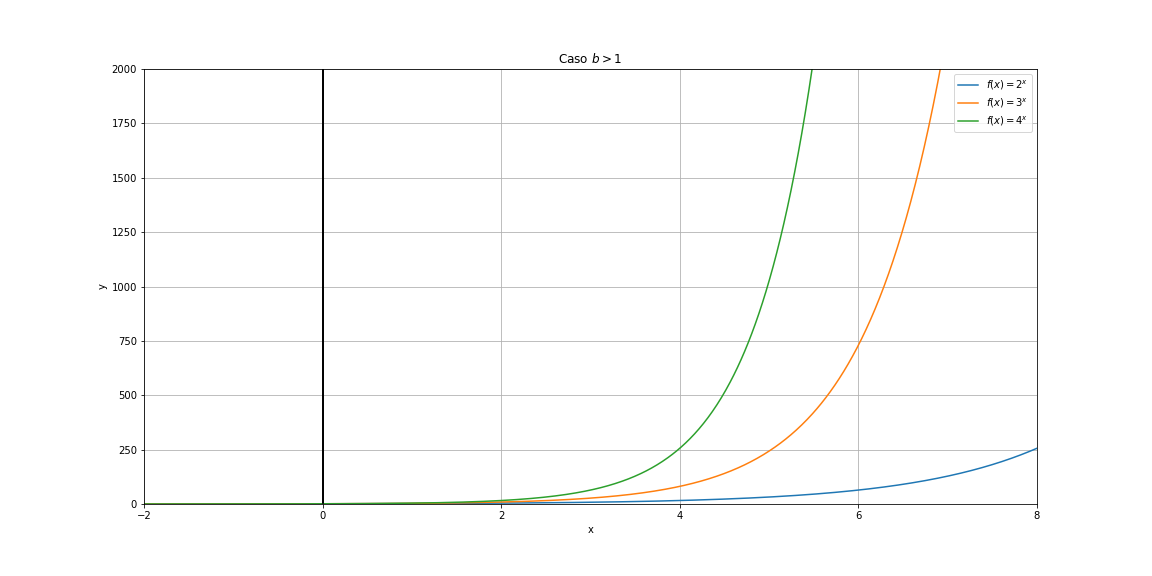
\includegraphics[scale=0.35]{expb0.png}
\caption[Gráfica de funciones exponenciales para el caso de la base $b>1$.]{Gráfica de funciones exponenciales para el caso de la base $b>1$. Se ve una función siempre creciente. El dominio son todos los reales y la imagen los reales positivos.} \label{expb0}
\end{figure}
\end{center}

 \begin{center}
\begin{figure}[h!]
\centering
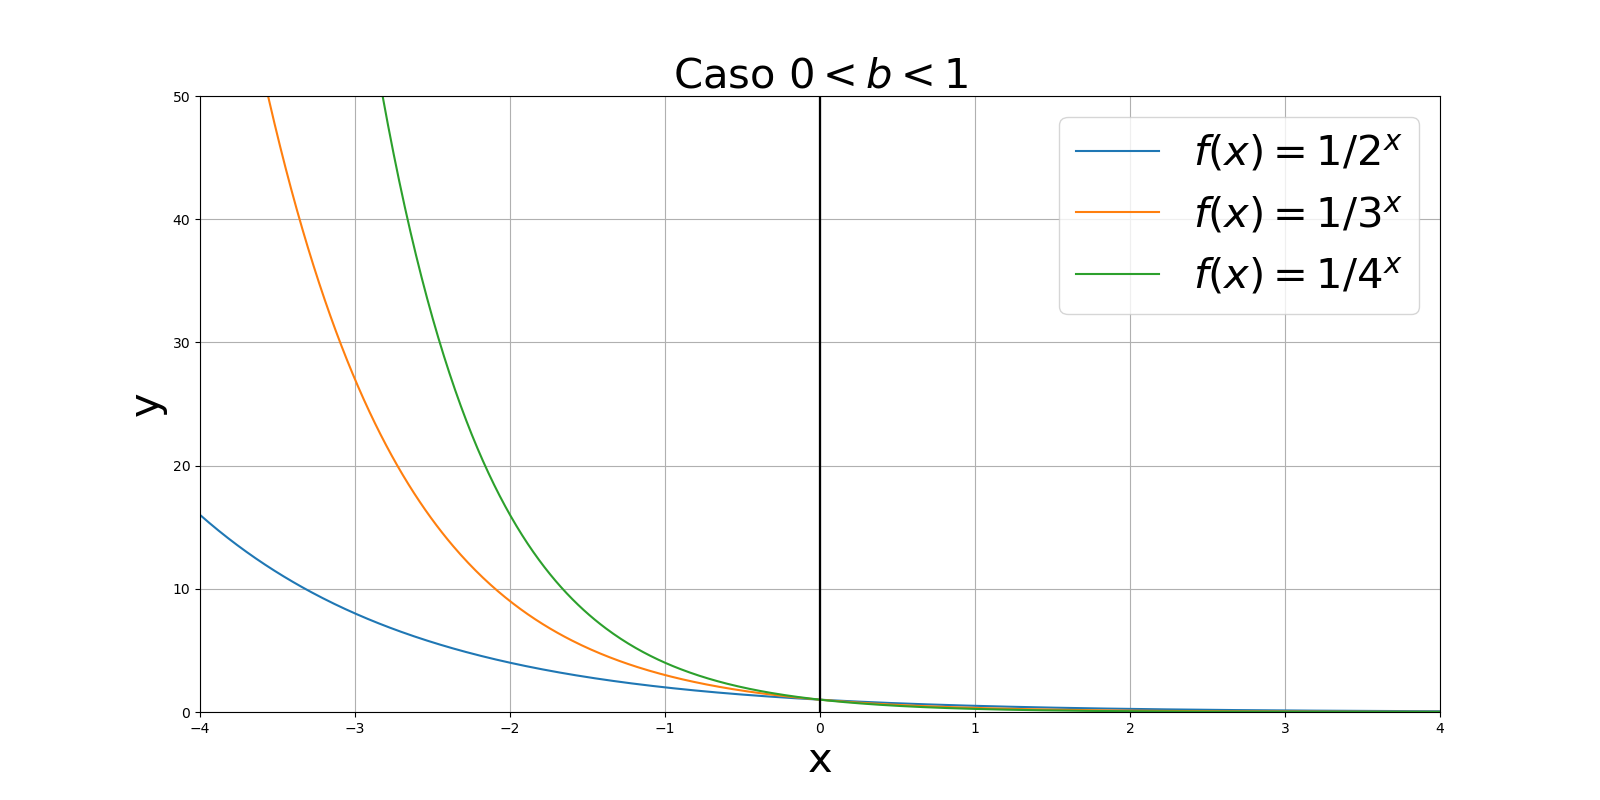
\includegraphics[scale=0.35]{expb1.png}
\caption[Gráfica de funciones exponenciales para el caso de la base $0<b<1$]{Gráfica de funciones exponenciales para el caso de la base $0<b<1$. Se ve una función siempre decreciente. El dominio son todos los reales y la imagen los reales positivos.} \label{expb1}
\end{figure}
\end{center}

De las figuras (\ref{expb0}) y (\ref{expb1}) se ve que las funciones exponenciales son uno a uno, continuas y que no cruzan el eje $x$. Adicionalmente, se puede dar el caso en que la función se desplaza, es decir, que al exponente se le suma un número, por ejemplo $4^{x+3}$ es una función desplazada de $4^{x}$. Dependiendo del caso, la función desplazada crece o decrece más rápido que la original.
\newpage
\subsection{Número e}

Un caso particular de base es el número $e$, que junto a $\pi$ son números particulares, ya que tienen decimales no repetitivos e infinitos. Una formar de representar estos números son series. Las series son sumas infinitas (se suman infinitos términos) de términos por medio de una expresión en común. 
\begin{eqnarray*}
e&=&1 + \dfrac{1}{1} + \dfrac{1}{1\cdot 2} + \dfrac{1}{1\cdot 2\cdot 3} + \dfrac{1}{1\cdot 2\cdot 3\cdot 4}+\cdots \\
&=&\dfrac{1}{0!} + \dfrac{1}{1!} + \dfrac{1}{ 2!} + \dfrac{1}{3!} + \dfrac{1}{4!}+\cdots \\
&=&\sum_{n=0}^{\infty}\dfrac{1}{n!}
\end{eqnarray*}
La notación $n!$ se le llama factorial y es la multiplicación de todos los números que hay desde $n$ hasta el $1$, el caso particular del del cero es $0!=1$. Para $n$ muy muy grandes ($n\rightarrow \infty$) el número $e$ tiende a la función
\begin{eqnarray*}
e&\rightarrow &\left(1+\dfrac{1}{x}\right)^{x} \\
e&=&2,7182818...
\end{eqnarray*} 
Por lo visto hay más de una forma para mostrar un simple número decimal (porque no deja de ser eso, un simple número decimal), pero muestra la importancia del número $e$ en la matemática.

\begin{mydef}
\textbf{Función exponencial natural. } Sea b la base de la función exponencial, entonces se elije $b=e$ y la función queda definida
\begin{eqnarray}
f(x)=e^{x}
\end{eqnarray}
\end{mydef}
Las gráficas de la función natural siguen la misma lógica de las figuras (\ref{expb0}) y (\ref{expb1}) cuando la base es $e$ y $1/e$ respectivamente. Puede ser desplazada verticalmente si se agrega una constante, por ejemplo $f(x)=c\pm e^{x}$.

Un caso en donde es muy usado el número $e$ es la en la función gaussiana, que en su forma más simple es $e^{-x^2}$. No cruza el eje $x$ y es simétrica  con respecto al eje $y$.
%Gráfica
\section{Funciones logarítmicas}

Las funciones exponenciales son uno a uno, por lo que debe existir una función vaya desde la imagen al dominio, es decir, una función inversa. Se introduce el concepto de logaritmo, por lo que la función logarítmica queda de la forma
\begin{mydef}
\textbf{Función logarítmica. } Con la base $b>0$, $b\neq 1$ se define por
\begin{eqnarray}
y=log_{b}(x), \hspace{10px} ssi \hspace{6px} x=b^{y}
\label{funlog0}
\end{eqnarray}
La abreviatura `ssi' es por la frase `si y solo si'. La función (\ref{funlog0})  se lee \textbf{y es el logaritmo de la base b que da como resultado x}.
\end{mydef}

En la función logarítmica $b>0$ no hay exponente $y$ que haga que la expresión $b^{y}$ sea menor que cero, en consecuencia, $x$ es mayor que cero. Entonces, el dominio de la función logarítmica son los números reales positivos.\\

Por el lado de las gráficas, ocurre igual que en las funciones exponenciales y se separan en dos casos según el valor de la base $b$. Se debe recordar que el dominio de las funciones exponenciales son todos los números reales y la imagen son los reales positivos. Entonces, como la función logarítmica es la inversa  de la función exponencial, los papeles se invierten.

 \begin{center}
\begin{figure}[h!]
\centering
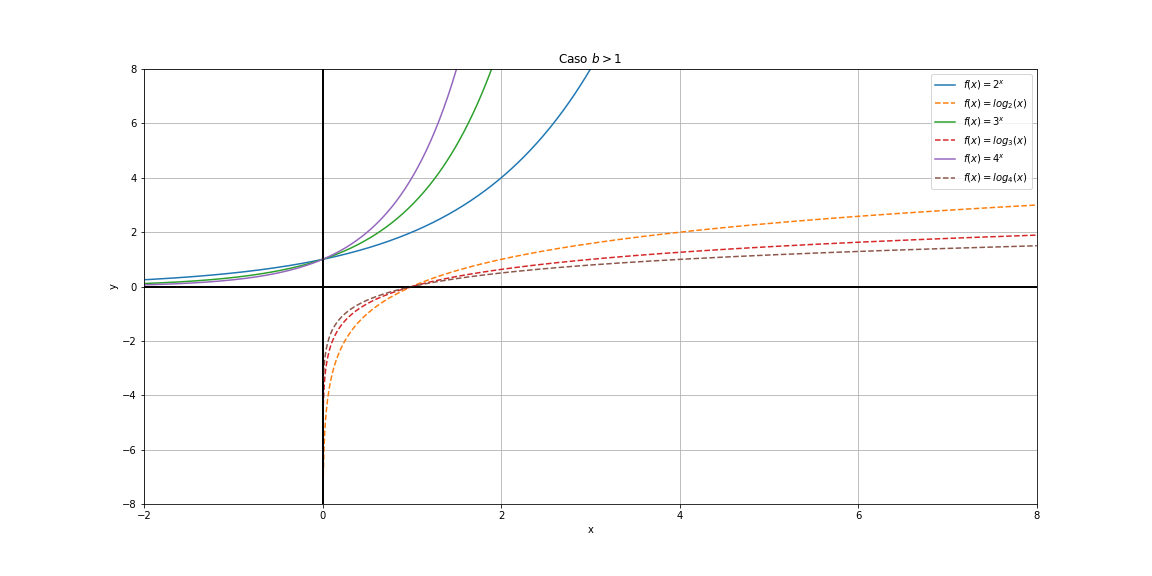
\includegraphics[scale=0.3]{logb0.png}
\caption[Gráfica de funciones logarítmicas para el caso de la base $b>1$]{Gráfica de funciones Logarítmicas para el caso de la base $b>1$. Notar que que se invierte el dominio con la imagen.} \label{logb0}
\end{figure}
\end{center}

 \begin{center}
\begin{figure}[h!]
\centering
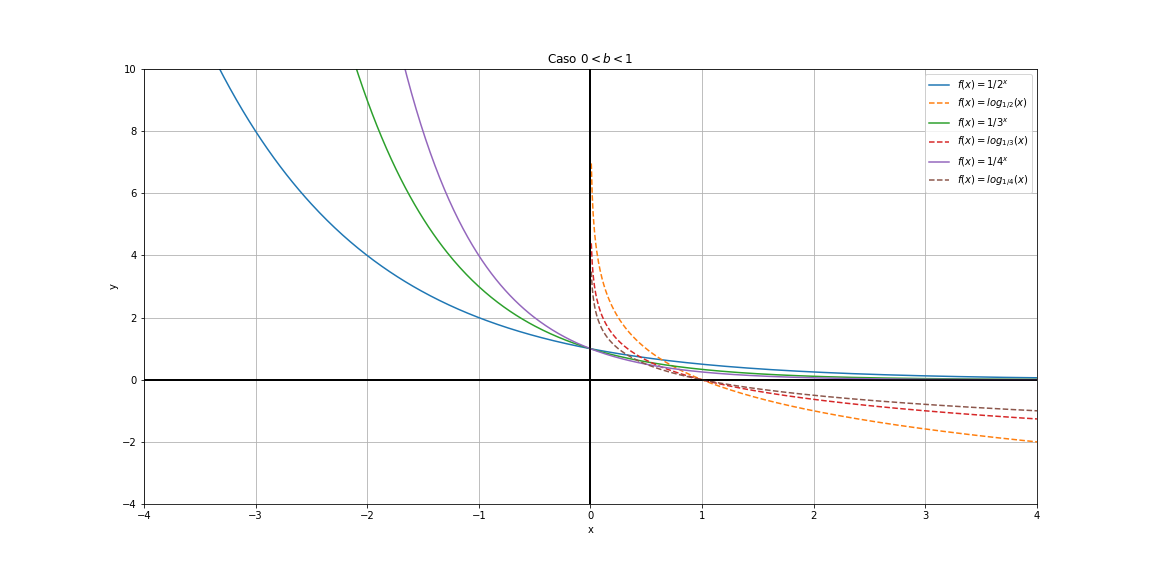
\includegraphics[scale=0.3]{logb1.png}
\caption[Gráfica de funciones logarítmicas para el caso de la base $0<b<1$]{Gráfica de funciones logarítmicas para el caso de la base $0<b<1$. Notar que se invierte el dominio con la imagen.} \label{logb1}
\end{figure}
\end{center}

Del las figuras (\ref{logb0}) y (\ref{logb1}) se ve que el eje $y$ es una asíntota vertical. Además, cuando el primer caso se va a $-\infty$ cuando se acerca el cero, mientras que para el segundo caso se va a $+\infty$. Entonces, algunas propiedades de la función logarítmica es que es uno a uno, es una función continua en el intervalo $]0,+\infty[$ y la intersección con el eje $x$ está en el punto $(1,0)$.\\

Hay un caso particular dentro del caso de la base $b>1$. Así como los logaritmos de base $10$ ($b=10$) se les llama comunes, a los logaritmos de base $e$ se les llama logaritmos naturales y su notación es $log_{e}(x)=ln(x)$. Entonces, ocurre que la expresión $ln(e)=1$ ya que $e^{1}=e$. Es una muestra más de que la función exponencial y la logarítmica son funciones inversas y las identidades quedan de la forma:
\begin{eqnarray}
x&=&e^{ln(x)}\\
y&=&ln(e^{y})
\end{eqnarray}
Lo que en palabras simples se traduce en que si tengo una función logarítmicas la puede eliminar con una función exponencial y viceversa. Para finalizar, mostraremos las leyes de los logaritmos
\newpage
\begin{mydef}
\textbf{Leyes de los logaritmos. } Para toda base $b>0$, $b\neq 1$, y para todos los números positivos $M$ y $N$.
\begin{itemize}
	\item $log_{b}(MN)=log_{b}(M)+log_{b}(N)$
	\item $log_{b}\left(\dfrac{M}{N}\right)=log_{b}(M)-log_{b}(N)$
	\item $log_{b}(M^{c})=c\cdot log_{b}(M)$, para cualquier número real c.\\
\end{itemize}
\end{mydef}

\begin{myexample}
Reducir el siguiente logaritmo:\\
\noindent\textit{i)}
\begin{eqnarray*}
ln(\sqrt{e})=ln(e^{1/2})=\dfrac{1}{2}ln(e)=\dfrac{1}{2}\cdot 1=\dfrac{1}{2}
\end{eqnarray*}
\noindent\textit{ii)}
\begin{eqnarray*}
log_{10}2\sqrt{2\sqrt{2\sqrt{2}}} &=&log_{10}2\left( 2\sqrt{2\sqrt{2}}\right)^{1/2}\\
 &=& log_{10}(2)+ log_{10}\left( 2\sqrt{2\sqrt{2}}\right)^{1/2}\\
 &=& log_{10}(2)+\dfrac{1}{2} log_{10}\left( 2\sqrt{2\sqrt{2}}\right)\\
  &=& log_{10}(2)+\dfrac{1}{2}\left[ log_{10}(2)+log_{10}\left( \sqrt{2\sqrt{2}}\right)\right]\\
    &=& log_{10}(2)+\dfrac{1}{2} log_{10}(2)+\dfrac{1}{2} log_{10}\left( \sqrt{2\sqrt{2}}\right)\\
    &=& log_{10}(2)+\dfrac{1}{2} log_{10}(2)+\dfrac{1}{2} log_{10}\left( 2\sqrt{2}\right)^{1/2}\\
     &=& \dfrac{3}{2} log_{10}(2)+\dfrac{1}{4} log_{10}\left( 2\sqrt{2}\right)\\
      &=& \dfrac{3}{2} log_{10}(2)+\dfrac{1}{4} log_{10}(2)+\dfrac{1}{4}log_{10}(2)^{1/2}\\
      &=& \dfrac{3}{2} log_{10}(2)+\dfrac{1}{4} log_{10}(2)+\dfrac{1}{8}log_{10}(2)\\
      &=& log_{10}(2)\left[\dfrac{3}{2}+\dfrac{1}{4}+\dfrac{1}{8} \right]\\
      &=& \dfrac{15}{8} log_{10}(2)\\
\end{eqnarray*}
\noindent\textit{iii)}
\begin{eqnarray*}
log_{10}\left(\dfrac{x^{4}y(w+z)}{wz} \right)&=& log_{10}\left(x^{4}y(w+z) \right)-log_{10}\left(wz \right)\\
&=& log_{10}(x^{4}y)+ log_{10}(w+z)-log_{10}\left(wz \right)\\
&=& log_{10}(x^{4})+log_{10}(y)+ log_{10}(w+z)-\left[ log_{10}(w)+log_{10}(z) \right]\\
&=& 4log_{10}(x)+log_{10}(y)+ log_{10}(w+z)-log_{10}(w)-log_{10}(z) \\
\end{eqnarray*}
\end{myexample}

\section{Ecuaciones exponenciales y logarítmicas}
Vistas las gráficas y propiedades de las funciones exponenciales y logarítmicas, ahora toca dar un paso adelante y es trabajar con las expresiones, pero agregando incógnitas. 

\begin{myexample}
Resolver la ecuación $e^{10x}=7$, encontrar el valor de x:\\

\noindent Sol: Primero, como la incógnita está en el exponente debemos encontrar una función que elimine la función exponencial, justamente es la logarítmica.
\begin{eqnarray*}
e^{10x}&=&7\\
10x&=&ln(7)\\
x&=&\dfrac{1}{10}ln(7)
\end{eqnarray*}
\end{myexample}

Una propiedad importante que viene de que las funciones logarítmicas y exponenciales son uno a uno es que $f(x_{1})=f(x_{2})$. Se puede utilizar esta herramienta para igualar términos y encontrar la incógnita.

\begin{mydef}
\textbf{Propiedades uno a uno de las funciones exponenciales y logarítmicas.} Sea $b$ la base de la función exponencial, con $b>0$, $b\neq 1$ y la función logarítmica $y=log_{b}(x)$. Se cumple que:
\begin{eqnarray}
Si\hspace{4px} b^{x_{1}} &=& b^{x_{2}},\hspace{4px} entonces\hspace{4px} x_{1}=x_{2}\\
Si\hspace{4px} log_{b}(x_{1})&=&log_{b}(x_{2}),\hspace{4px} entonces\hspace{4px} x_{1}=x_{2}
\end{eqnarray}
\end{mydef}

\begin{myexample}
Encontrar el valor de x de las siguientes ecuaciones:\\

\noindent\textit{i)}
\begin{eqnarray*}
7^{2(x+1)}&=&343\\
7^{2(x+1)}&=&7^{3}\\
2(x+1)&=&3\\
2x+2&=&3\\
2x&=&1\\
x&=&\dfrac{1}{2}
\end{eqnarray*}
\end{myexample}
\noindent\textit{ii)}
\begin{eqnarray*}
ln(2)+ln(4x-1)&=&ln(2x+5)\\
ln(2(4x-1))&=&ln(2x+5)\\
2(4x-1)&=&2x+5\\
8x-2&=&2x+5\\
6x&=&7\\
6x&=&7\\
x&=&\dfrac{7}{6}\\
\end{eqnarray*}

\section{Modelos matemáticos exponenciales y logarítmicos}

El paso que corona los conceptos vistos en las secciones anteriores, son los modelos matemáticos que se usan con estas funciones. Primero, para entender lo que es un modelo en palabras simples, es una expresión que \textit{intenta} describir matemáticamente un fenómeno. Este suceso no tiene por qué ser representando al $100\%$ por el modelo, porque puede estar echo para hacer cálculos futuros o tener una idea simple de lo que ocurre. Los modelos pueden ser tan simples o tan complejos como uno quiera y un factor que ayuda a los modelos son los \textit{parámetros}. Estas variables pueden ser constantes universalmente conocidas o números que cambian en el modelo según el caso que uno considere, dando un grado de realidad al modelo.

\subsection{Modelos matemáticos exponenciales}
Si hablamos de modelos exponenciales, es porque  la incógnita se encuentra en el exponente y un fenómeno descrito por estas funciones es el crecimiento de una población. Se debe agregar las constantes que condiciona la situación.
\begin{eqnarray}
P(t)=P_{0}e^{kt}, \hspace{6px} k>0 
\end{eqnarray} 
El término $P(t)$ nos dice que la incógnita es $t$, es decir, el tiempo. Por lo que el modelo nos dice cuanta población habrá en un tiempo determinado. La constante $P(0)$ se llama población inicial y se condiciona a la cantidad población que hay en el tiempo cero ($t=0$). Por último, la constante $k$ se llama tasa de crecimiento y nos dice que tan rápido crece, notar que si $k<0$ sería de decrecimiento. 
\newpage
\begin{myexample}
La bacteria Escherichia coli (E. coli) duplica su población en 20 minutos. Usar el modelo exponencial para calcular la población de bacterias después de 6 horas.\\

\noindent Sol: Lo primero en todo problema es asegurarse que todos los datos estén en la misma unidad de medida, entonces pasaremos los minutos a horas. Tiempo de duplicación de población $20min=1/3h$. Por otro lado, en este problema no se especifica nada sobre la población inicial, por lo que la dejaremos con el símbolo.\\

Notar que en $t=1/3$ la bacteria duplica su población, es decir, $P(1/3)=2P_{0}$ y reemplazando $t$ en el modelo queda:
\begin{eqnarray*}
P(1/3)&=&  2P_{0}\\
P_{0}e^{k/3}&=&2P_{0}\\
e^{k/3}&=&2\\
\dfrac{k}{3}&=&ln(2)\\
k&=&3\cdot ln(2)\\
\end{eqnarray*}
Ahora ya tenemos el valor de la constante $k$, entonces lo reemplazamos en el modelo
\begin{eqnarray*}
P(t)&=&P_{0}e^{3\cdot ln(2)\cdot t}\\
P(t=6)&=&P_{0}e^{3\cdot ln(2)\cdot 6}\\
P(t=6)&=&P_{0}e^{18\cdot ln(2) }\\
P(t=6)&=&P_{0}\cdot 262144
\end{eqnarray*}
Ahora uno puede poner casos particulares de la población inicial ($P_{0}$) y multiplicarlo por $262144$, que es la población de la bacteria luego de $6$ $horas$.
\end{myexample}

\begin{myexample}
Se necesita estudiar el crecimiento de dos tipos de bacterias, $P_{1}$ y $P_{2}$. La primera alcanza la población de $10.000$ en $4$ horas y la segunda comienza con el doble de la población respecto a la primera, además la segunda alcanza la población de $10.000$ en $3$ horas. Con el modelo exponencial encuentre la población inicial ($P_{0}$) de cada bacteria. Se asume el parámetro de crecimiento $k$ es el mismo para ambas bacterias
\end{myexample}
Expresiones para ambas bacterias:
\begin{eqnarray}
P_{1}(t)= P_{0}e^{kt} &y& P_{2}=2P_{0}e^{kt}
\label{bac}
\end{eqnarray}
Expresiones en que la población de ambas bacterias es de $10.000$:
\begin{eqnarray*}
P_{1}(t=4)=10000 &y& P_{2}(t=3)=10000 \\
P_{0}e^{4k}&=&2P_{0}e^{3k}=10000\\
e^{4k}&=&2e^{3k}\hspace*{90px} / \cdot e^{-3k}\\
e^{k}&=&2\hspace*{105px} / ln()\\
ln(e^{k})&=&ln(2)\\
k&=& ln(2)
\end{eqnarray*}
Encontrado el parámetro k (que es el mismo para ambas bacterias), se reemplaza en (\ref{bac}) y se obtiene:
\begin{eqnarray*}
P_{1}(t)= P_{0}e^{ln(2)t} &y& P_{2}=2P_{0}e^{ln(2)t}
\end{eqnarray*}
y las expresiones cuando alcanzar las $10000$ bacterias son:
\begin{eqnarray*}
10000= P_{0}e^{4\cdot ln(2)} &y& 10000=2P_{0}e^{3\cdot ln(2)}\\
10000= P_{0}e^{4\cdot ln(2)} &y& 5000=P_{0}e^{3\cdot ln(2)}\\
10000= P_{0}e^{ ln(16)} &y& 5000=P_{0}e^{ln(8)}\\
P_{0}=\dfrac{10000}{e^{ln(16)}} &y& P_{0}=\dfrac{5000}{e^{ln(8)}}\\
P_{0}&=&625
\end{eqnarray*}
Como la población inicial es $P_{0}=625$ unidades. Entonces la bacteria uno, $P_{1}$, comenzó con $625$ de población inicial y la bacteria dos, $P_{2}$, con $1250$ unidades.
\subsection{Modelos matemáticos logarítmicos}

Una aplicación muy interesante donde aplicar los logaritmos, en base 10 en este caso, es en la escala de Ricther. Esta escala compara las energías de distintos sismos. 
\begin{eqnarray}
M=log_{10}\left(\dfrac{A}{A_{0}}\right)
\end{eqnarray}
M es la magnitud del sismo y $A_{0}$ es una amplitud de referencia que corresponde a la magnitud $M=0$

\begin{mydef}
En el año 1960 en la ciudad de Valdivia en Chile, ocurrió un terremoto de grado $9,6$ en la escala de Richter. En el año 2010 en Concepción en Chile, hubo un terremoto de grado $8,8$. Entonces ¿Cuántas veces más intenso fue el terremoto del año 1960 con respecto al del 2010?\\

\noindent Sol: Primero definimos las expresiones que le corresponde a cada terremoto
\begin{eqnarray*}
9,6=log_{10}\left(\dfrac{A}{A_{0}}\right)_{1960} \hspace{5px} y \hspace{5px}8,8=log_{10}\left(\dfrac{A}{A_{0}}\right)_{2010}
\end{eqnarray*}
Si se aplica la función logarítmica los términos queda de la forma
\begin{eqnarray*}
\left(\dfrac{A}{A_{0}}\right)_{1960}&=&10^{9,6} \hspace{5px} y \hspace{5px} \left(\dfrac{A}{A_{0}}\right)_{2010} = 10^{8,8}\\
\left(\dfrac{A}{A_{0}}\right)_{1960}&=&10^{9,6}=10^{8,8}\cdot 10^{0,8}\\
\left(\dfrac{A}{A_{0}}\right)_{1960}&=&10^{0,8}\left(\dfrac{A}{A_{0}}\right)_{2010}\\
\left(\dfrac{A}{A_{0}}\right)_{1960}&\approx & 6,3\left(\dfrac{A}{A_{0}}\right)_{2010}
\end{eqnarray*}
Entonces, el terremoto del año $1960$ en Valdivia fue más de $6$ veces más fuerte que el terremoto del año $2010$ en Concepción.
\end{mydef}

\subsection{Escalas logarítmicas y lineales}
Al ver las funciones logarítmicas y exponenciales se puede notar que no siempre es lo más optimo ocupar la \textit{escala usual}.  Comúnmente se una la escala lineal en los gráficos, que tiene la misma distancia entre los puntos que delimitan el gráfico (la distancia que hay entre en 1 y el 2, es la misma que hay entre el 2 y el 3 y así sucesivamente). Hay otras escalas que representan mejor algunas funciones, como por ejemplo las logarítmicas. Esta escala tiene como etiquetas los números $10^{n}$, siendo $n$ un número entero positivo o negativo, por lo que la etiqueta es siempre positiva.\\
Como resumen de estas escalas, es que son importante o son útiles usarlas cuando el rango de los datos es muy amplia.\\

A continuación mostramos algunos ejemplos de diferentes funciones graficadas en cuatros escalas distintas. De izquierda a derecha y de arriba a abajo es: Escala lineal, escala logarítmica en $x$ o semilog en $x$ (esto quiere decir que se utiliza escala logarítmica solo en el eje $x$), escala logarítmica en $y$ o semilog $y$ y escala logarítmica (escala logarítmica tanto en $x$ como en $y$).\\



 \begin{center}
\begin{figure}[h!]
\centering
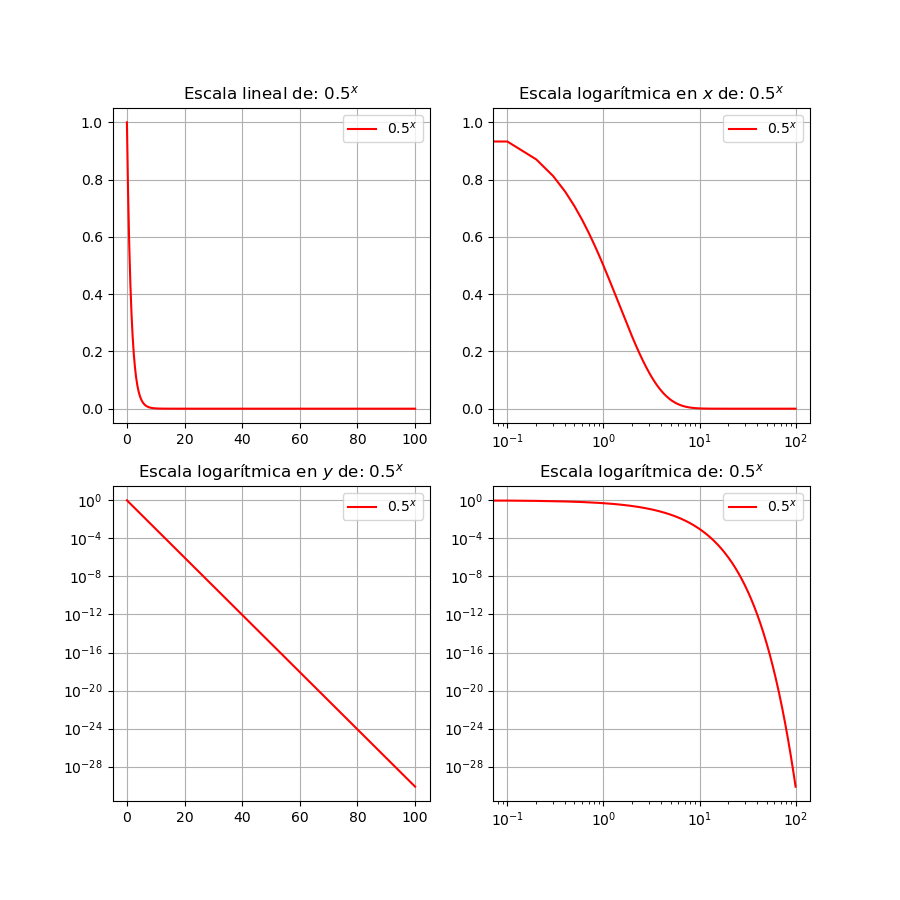
\includegraphics[scale=0.4]{Func0.png}
\caption[Cuatro escalas de la función $0.5^{x}$]{Cuatro escalas de la función $0.5^{x}$.} \label{func00}
\end{figure}
\end{center}

 \begin{center}
\begin{figure}[h!]
\centering
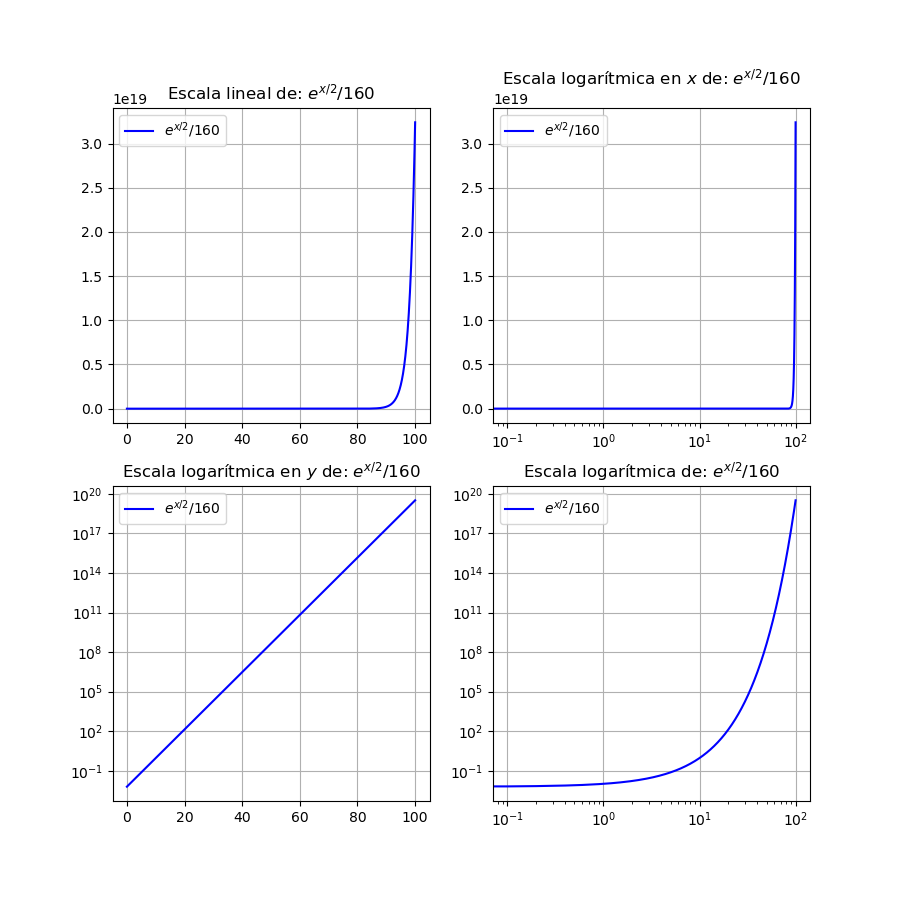
\includegraphics[scale=0.4]{Func1.png}
\caption[Cuatro escalas de la función $e^{x/2}/160$]{Cuatro escalas de la función $e^{x/2}/160$.} \label{func01}
\end{figure}
\end{center}

 \begin{center}
\begin{figure}[h!]
\centering
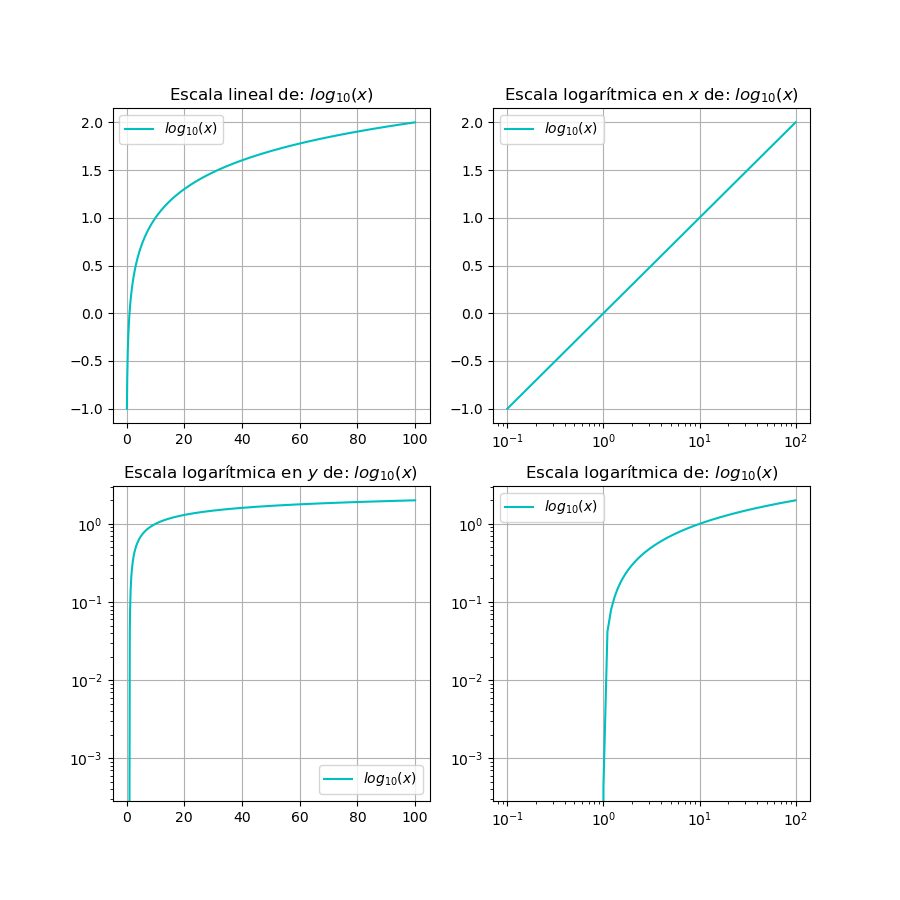
\includegraphics[scale=0.4]{Func2.png}
\caption[Cuatro escalas de la función $log_{10}(x)$]{Cuatro escalas de la función $log_{10}(x)$.} \label{func02}
\end{figure}
\end{center}

% \begin{center}
%\begin{figure}[h!]
%\centering
%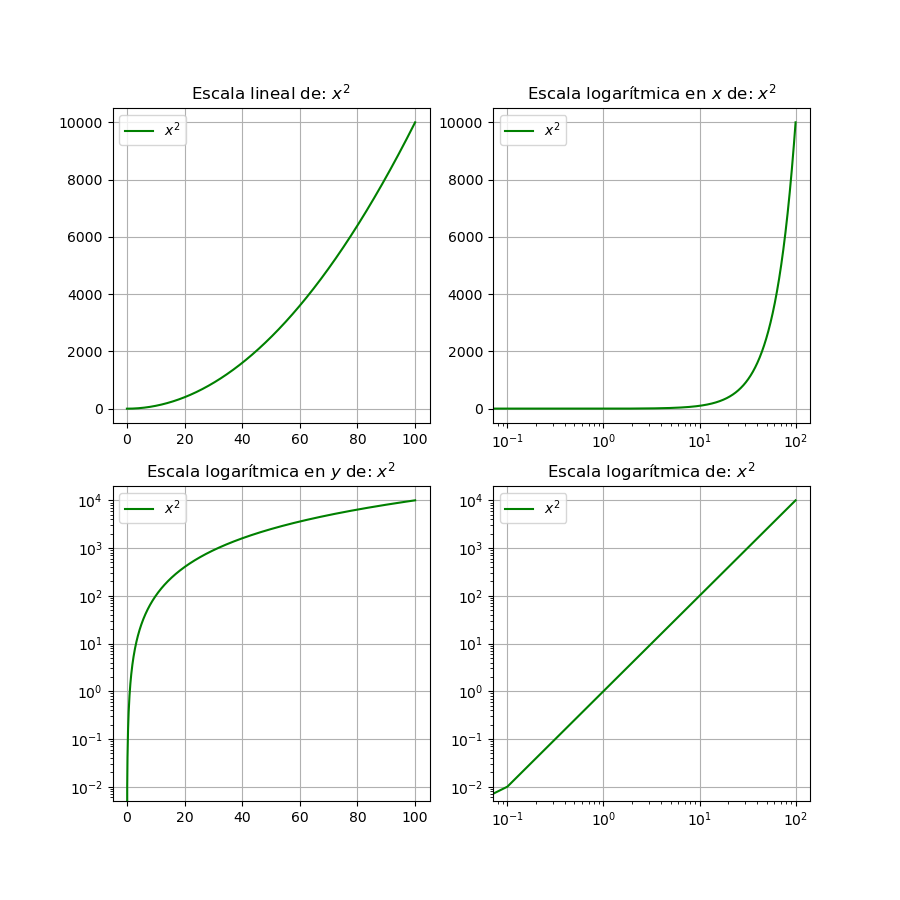
\includegraphics[scale=0.45]{Func3.png}
%\caption[Cuatro escalas de la función $x^{2}$]{Cuatro escalas de la función $x^{2}$.} \label{func03}
%\end{figure}
%\end{center}
	\rhead[\thepage]{\scriptsize{CAPÍTULO \thechapter}. \rightmark}
\lhead[CAPÍTULO \thechapter. \leftmark]{}
%======================================================================
\chapter{Cálculo vectorial}
\label{CV}
\markboth{Cálculo vectorial}{Cálculo vectorial}
%======================================================================

Este capítulo tiene como objetivo comprender el cálculo vectorial, que ayuda a tener una noción mayor sobre el espacio en donde se mueven las cosas. Un vector tiene como elementos que lo describen una magnitud y una dirección. Ejemplos del uso de vectores es muy amplio sobretodo en física, por ejemplo desplazamiento, velocidad, fuerza, etc.\\

Antes de llegar a los vectores como tal se debe ver ciertos temas, para tener una base sólida al momento de enfrentarse a problemas vectoriales, uno de ellos son los ángulos y su sentido.   
%----------------------------------------------------------------------
\section{Ángulos y su orientación}
\label{CV0}
%----------------------------------------------------------------------
El ángulo se forma con dos rectas con un punto en común que se llama \textit{vértice}. Uno puede imaginar que una de las rectas queda fija (lado inicial) y la otra recta (lado terminal) rota con respecto al vértice para formar el ángulo entre las dos rectas.\\
Cuando se forma el ángulo se puede medir en grados que van desde $0$ a $360$ grados y se considera positivo cuando va en sentido antihorario, por consiguiente, si va en sentido horario la medida será negativa.

 \begin{center}
\begin{figure}[h!]
\centering
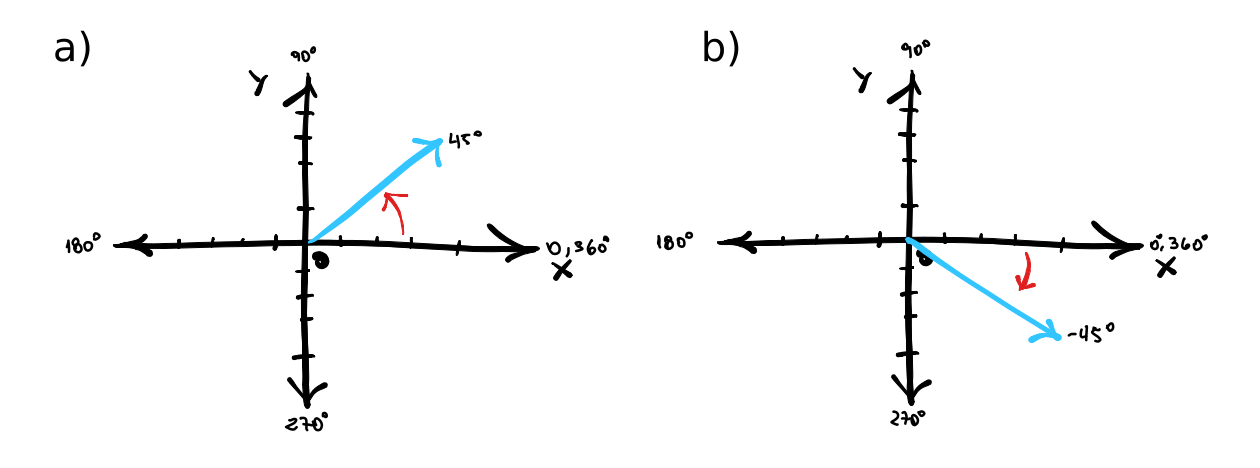
\includegraphics[scale=0.28]{ang0.png}
\caption[Figura de ángulos positivo y negativo]{Figura de ángulos positivo y negativo. a) Muestran un plano cartesiano de $x$ e $y$ donde hay un vector en $45^{o}$ en sentido positivo. b) Es un vector en el mismo plano cartesiano y también es de $45^{o}$, pero es negativo.} \label{grados0}
\end{figure}
\end{center}
Así como un ángulo se puede medir en grados, igual está la opción de medirlos en radianes. Esta unidad se basa en la longitud de un arco del un circulo centrado en el origen y de radio $1$.
\begin{eqnarray}
x^{2}+y^{2}=1
\end{eqnarray}
La convención en radianes son las mismas que en los ángulos, es decir, el sentido positivo y negativo son los mismos. Los radianes van desde $0$ a $2\pi$.

 \begin{center}
\begin{figure}[h!]
\centering
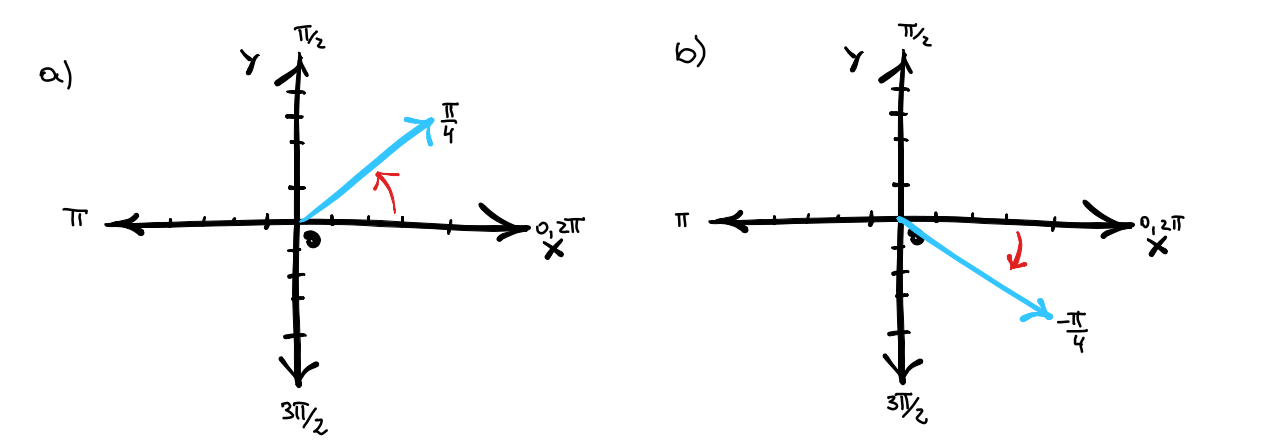
\includegraphics[scale=0.28]{ang1.png}
\caption[Figura de radianes positivo y negativo]{Figura de ángulos positivo y negativo. a) Muestran un plano cartesiano de $x$ e $y$ donde hay un vector en $\pi/4$ radianes en sentido positivo. b) Es un vector en el mismo plano cartesiano y también es de $\pi/4$ radianes, pero es negativo.} \label{grados0}
\end{figure}
\end{center}

La forma para pasar de un sistema al otro es hacer una regla de tres simples, siempre teniendo en cuenta que las equivalencias son las siguientes:
\begin{eqnarray*}
2\pi\rightarrow 360^{o}\\
x\rightarrow 45^{0}
\end{eqnarray*}
Por ejemplo, en esta regla de tres simples se quiere pasar de grados a radianes, entonces la incógnita es a cuantos radianes equivalen $45^{o}$. La respuesta es $x=\pi/4$.

El resumen de los ángulos más importantes se ven en la siguiente tabla;


\begin{table}[h!]
\begin{center}
 \begin{tabular}{|c|c|c|c|c|c|c|c|c|c|}
 \hline
 Grados $[^{o}]$ &$0$&$30$&$45$&$60$&$90$&$180$&$270$&$360$ \\
 \hline
 Radianes $[rad]$ &$0$&$\dfrac{\pi}{6}$&$\dfrac{\pi}{4}$&$\dfrac{\pi}{3}$&$\dfrac{\pi}{2}$&$\pi$&$\dfrac{3\pi}{2}$&$2\pi$ \\
 \hline
 \end{tabular}
 \caption{Tabla resumen de los ángulos más comunes en grados y su equivalente en radianes.}
 \end{center}
\end{table}

\section{Trigonometría}

Utilizaremos los ángulos mostrados en la sección anterior en funciones trigonométricas, que se pueden calcular en base a los lados de un triángulo rectángulo.\\
El triángulo rectángulo consta de 3 lados etiquetados con las letras $a$, $b$ y $c$. Además, se etiqueta un ángulo con la letra griega \textit{theta} $\theta$. El lado opuesto al ángulo recto se llama hipotenusa, el cateto que se une en un vértice con la hipotenusa y además contiene el ángulo $\theta$ se llama cateto adyacente y el cateto que no contiene al ángulo $\theta$ es el cateto opuesto.

\begin{center}
\begin{figure}[h!]
\centering
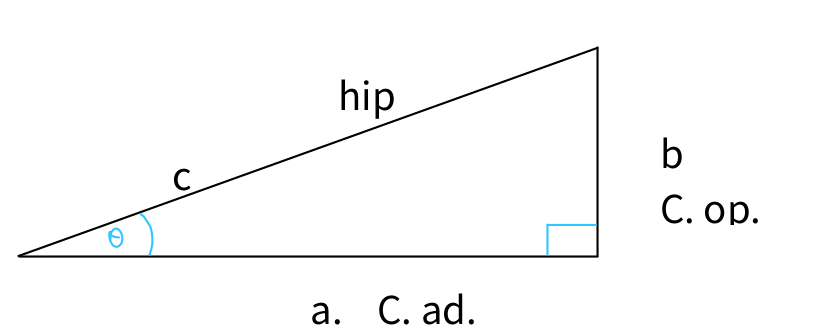
\includegraphics[scale=0.30]{trig0.png}
\caption[Triangulo rectángulo con las etiquetas sus catetos e hipotenusa]{Triángulo rectángulo con las etiquetas sus catetos e hipotenusa. El lado a es el cateto adyacente, b es el cateto opuesto y c es la hipotenusa. El ángulo entre el cateto adyacente y la hipotenusa se etiqueta con $\theta$. } \label{trig0}
\end{figure}
\end{center}

\begin{mydef}
\textbf{Funciones trigonométricas. }En base al triangulo de la figura (\ref{trig0}) se definen las siguientes funciones trigonométricas:
\begin{eqnarray}
sen(\theta)&=&\dfrac{C. op.}{hip}\\
cos(\theta)&=&\dfrac{C. ad.}{hip}\\
tan(\theta)&=&\dfrac{C. op}{C. ad}=\dfrac{sen(\theta)}{cos(\theta)}\\
cot(\theta)&=&\dfrac{C. ad}{C. op}=\dfrac{1}{tan(\theta)}\\
sec(\theta)&=&\dfrac{hip}{C. ad.}=\dfrac{1}{cos(\theta)}\\
csc(\theta)&=&\dfrac{hip}{C. op}=\dfrac{1}{sen(\theta)}
\end{eqnarray}
Las abreviaciones son las siguientes: sen=seno, cos=coseno, tan=tangente, cot=cotangente, sec=secante y csc=cosecante.
\end{mydef}

El triángulo de la figura (\ref{trig0}) al ser rectángulo cumple el teorema de Pitágoras, entonces se puede usar para formular las soguientes identidades trigonométricas. 
\begin{eqnarray}
a^{2}+b^{2}=c^{c}
\label{pitagoras}
\end{eqnarray} 
Si (\ref{pitagoras}) lo dividimos por $a^{2}$, $b^{2}$ y $c^{c}$ se obtienen las siguientes ecuaciones.\\

\noindent a) Dividir por $c^{2}:$
\begin{eqnarray}
a^{2}+b^{2}=c^{c} \\
\left(\dfrac{a}{c}\right)^{2}+\left(\dfrac{b}{c}\right)^{2}=1
\end{eqnarray}

\noindent a) Dividir por $b^{2}:$
\begin{eqnarray}
a^{2}+b^{2}=c^{c} \\
\left(\dfrac{a}{b}\right)^{2}+1=\left(\dfrac{c}{b}\right)^{2}
\end{eqnarray}

\noindent a) Dividir por $a^{2}:$
\begin{eqnarray}
a^{2}+b^{2}=c^{c} \\
1+\left(\dfrac{b}{a}\right)^{2}=\left(\dfrac{c}{a}\right)^{2}
\end{eqnarray}
Si las ecuaciones anteriores lo pasamos a funciones trigonométricas se forman las siguientes identidades

\begin{mydef}
\textbf{Identidades trigonométricas. }
\begin{eqnarray}
sen^{2}(\theta)+cos^{2}(\theta)=1\\
1+tan^{2}(\theta)=sec^{2}(\theta)\\
cot^{2}(\theta)+1=csc^{2}(\theta)
\end{eqnarray}
\end{mydef}

Si se junta las funciones trigonométricas con lo visto de los ángulos en grados y radianes se puede resumir en una tabla con los valores más comunes.

\begin{table}[h!]
\begin{center}
 \begin{tabular}{|c|c|c|c|c|c|c|c|}
 \hline
Grados &$0^{o}$&$30^{o}=\pi/6$&$45^{o}=\pi/4$&$60^{o}=\pi/3$&$90^{o}=\pi/2$&$270^{o}=3\pi/2$ \\
 \hline
 $sen(\theta)$&$0$&$\dfrac{1}{2}$&$\dfrac{\sqrt{2}}{2}$&$\dfrac{\sqrt{3}}{2}$&$1$&$-1$ \\
 \hline
 $cos(\theta)$&$1$&$\dfrac{\sqrt{3}}{2}$&$\dfrac{\sqrt{2}}{2}$&$\dfrac{1}{2}$&$0$&$0$ \\
 \hline
 $tan(\theta)$&$0$&$\dfrac{\sqrt{3}}{3}$&$1$&$\sqrt{3}$&$\infty$&$\infty$ \\
 \hline
 \end{tabular}
 \caption{Tabla resumen de los valores mas comunes de las funciones trigonométricas.}
 \end{center}
\end{table}

\begin{myexample}
Encuentre el valor de la siguiente expresión:
\begin{eqnarray*}
cos(30^{o})\cdot tan(60^{o})=\dfrac{\sqrt{3}}{2}\cdot\sqrt{3}=\dfrac{3}{2}
\end{eqnarray*}
\end{myexample}

\section{Vectores}

Cuando uno se enfrenta a los problemas de mover cosas o desplazarse, uno hace un mapa o plano mental de como moverse y de forma inconsciente hacemos las direcciones. Si se plasma ese plano mental, naturalmente lo llevaremos a \textit{flechas} que nos direccionan a nuestro destino. Estas flechas con un largo y dirección lo llamaremos \textit{vector}.\\

Gráficamente, el vector es representado por una flecha entre dos puntos, donde tiene un punto inicial y final que define su dirección. Si los puntos que son $O$ y $P$ el trazo $OP$ forma el vector denotado por $\vec{A}$ y el largo del vector se llama magnitud y es denotado $|\vec{A}|$.\\

 \begin{center}
\begin{figure}[h!]
\centering
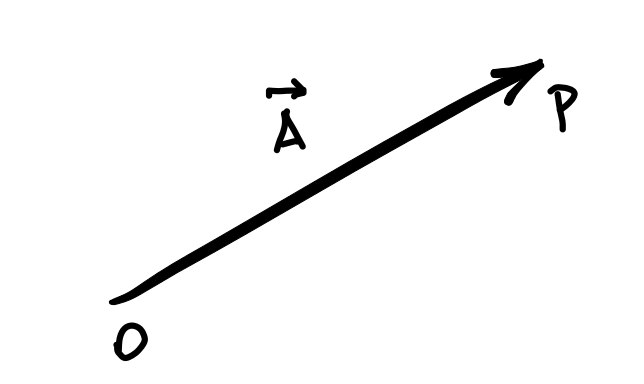
\includegraphics[scale=0.30]{vect0.png}
\caption[Representación de un vector.]{Representación de un vector. El punto inicial es el $O$, el punto final es el $P$ y el largo es la magnitud.} \label{vect0}
\end{figure}
\end{center}

La magnitud es un número y no tiene dirección, a estas cantidades se les llama \textit{escalares}. Ejemplos de magnitudes escalares son: La masa, largo, tiempo, temperatura y cualquier cantidad que sea un número real.

\begin{eqnarray}
\vec{A}=|\vec{A}|\cdot\vec{e}
\label{vector0}
\end{eqnarray}
El vector $\vec{A}$ cuenta con un número escalar que es la magnitud y un vector que le da la dirección. Un ejemplo que sirve por el momento es decir que uno se puede mover $10m$, pero es distinto decir que uno se moverá $10m$ al sur o al norte. El decir norte o sur da la dirección a la cual uno se desplazará.
\begin{itemize}
	\item Sea $\vec{A}$ y $\vec{B}$ dos vectores y se dicen que son iguales si tienen la misma magnitud y dirección sin importar sus puntos de inicio. Ver representación a) de la figura (\ref{vect1}).\\
	\item Un vector $\vec{A}$, pero con dirección opuesta y misma magnitud se denota como $-\vec{A}$. Ver representación b) de la figura (\ref{vect1}).
\end{itemize}

 \begin{center}
\begin{figure}[h!]
\centering
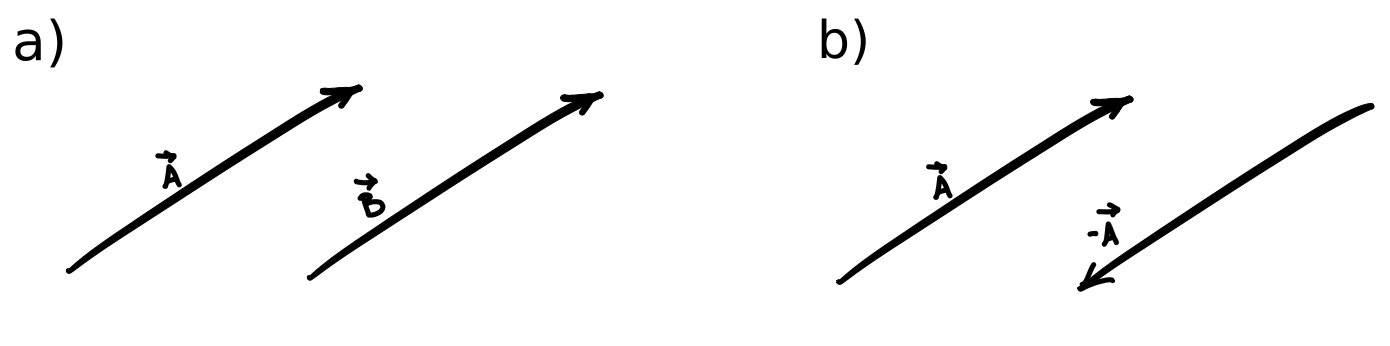
\includegraphics[scale=0.25]{vect1.png}
\caption[Representación 
Representación de vectores iguales y opuestos.]{Representación de vectores iguales y opuestos. a) Se muestran dos vectores iguales que son iguales en magnitud y sentido. b) Se muestran dos vectores opuestos que son iguales en magnitud pero distintos en sentido.} \label{vect1}
\end{figure}
\end{center}

Las operaciones posibles con los vectores son la suma, la resta y la multiplicación. Por parte de la suma de dos vectores se forma un vector resultante donde el inicio calza con el inicio del primer vector y termina con el punto final del segundo vector. En la resta se une ambos puntos finales de los vectores (ver figura \ref{vect2}).

 \begin{center}
\begin{figure}[h!]
\centering
\includegraphics[scale=0.25]{vect2.png}
\caption[Representación de la suma y resta de dos vectores.]{Representación de la suma y resta de dos vectores. Se muestran los vectores $\vec{A}$ y $\vec{B}$ donde son duplicados para mostrar como es el vector resultante de la suma y la resta de ellos mismo.} \label{vect2}
\end{figure}
\end{center}

En términos matemáticos, cuando se aplica la operación de suma o resta se debe aplicar en cada un de los elementos. La primera forma de ver un vector en más de una dimensión es un paréntesis donde cada número representa la magnitud que tiene en cada dirección. Entonces, considere dos vectores $\vec{v}_{1}=(x_{1},y_{1},z_{1})$ y $\vec{v}_{2}=(x_{2},y_{2},z_{2})$ donde la suma y la resta queda definida como:\\

\noindent a) Suma:\\
\begin{eqnarray}
\vec{v}_{1}+\vec{v}_{2}&=&(x_{1},y_{1},z_{1})+(x_{2},y_{2},z_{2})\\
&=&(x_{1}+x_{2},y_{1}+y_{2},z_{1}+z_{2})
\end{eqnarray}
\noindent a) Resta:\\
\begin{eqnarray}
\vec{v}_{1}-\vec{v}_{2}&=&(x_{1},y_{1},z_{1})-(x_{2},y_{2},z_{2})\\
&=&(x_{1}-x_{2},y_{1}-y_{2},z_{1}-z_{2})
\end{eqnarray}

\begin{mydef}
\textbf{Algebra de los vectores. }Si $\vec{A}$, $\vec{B}$ y $\vec{C}$ son vectores y $m$ y $n$ son escalares, entonces se cumple las siguientes leyes:
\end{mydef}
\begin{eqnarray}
\vec{A}+\vec{B}&=&\vec{B}+\vec{A}\\
\vec{A}+(\vec{B}+\vec{C})&=&(\vec{A}+\vec{B})+\vec{C}\\
m\vec{A}&=&\vec{A}m\\
m(n\vec{A})&=&(mn)\vec{A}\\
(m+n)\vec{A}&=&m\vec{A}+n\vec{A}\\
m(\vec{A}+\vec{B})&=&m\vec{A}+m\vec{B}
\end{eqnarray}



\subsection{Vectores unitarios}

En la ecuación (\ref{vector0}) presentamos a $\vec{e}$ que nos dice la dirección del vector. Este elemento se le llama vector unitarios, es decir, tiene largo uno.\\
Cuando creamos un plano en 2D o un espacio en 3D para colocar los vectores, cada eje tiene un vector unitario. A diferencia de cualquier vector, la notación de un vector unitario es $\hat{i}, \hat{j}$ y $\hat{k}$.

 \begin{center}
\begin{figure}[h!]
\centering
\includegraphics[scale=0.25]{vect3.png}
\caption[Representación de los vectores unitarios.]{Representación de los vectores unitarios. Se muestra que el largo de cada uno de los vectores es 1 partiendo desde el origen.} \label{vect3}
\end{figure}
\end{center}

\begin{myexample}
Sea $\vec{A}=5\hat{i}$, calcule el doble del vector $\vec{A}$.
\begin{eqnarray*}
\vec{A}&=&5\hat{i}\\
2\cdot\vec{A}&=&2\cdot 5\hat{i}\\
2\cdot\vec{A}&=&10\hat{i}\\
\end{eqnarray*}
\end{myexample}

Ahora cualquier vector se puede  volver un vector unitario. Si un vector $\vec{A}$ tiene una norma distinta de uno, se debe dividir por un escalar y es su propia magnitud.
\begin{eqnarray}
\vec{A}=\dfrac{\vec{A}}{|\vec{A}|}
\end{eqnarray}

\subsection{Componentes de un vector}

Así como en un principio se dijo que era importante decir la dirección del vector, si era sur o norte, pero que ocurre si la dirección es Noroeste. El vector tiene una parte hacia el norte y una parte hacia el oeste. En estos vectores se dice que tiene componentes en esas direcciones. Si generalizamos con los ejes que hemos planteado un vector puede tener componentes en los ejes $\hat{i}, \hat{j}$ y $\hat{k}$. Esto se puede extender a cuantas componentes nosotros queramos, pero para este curso veremos el caso de dos y tres dimensiones.
\begin{eqnarray}
\vec{A}=A_{1}\hat{i}+A_{2}\hat{j}+A_{3}\hat{k}
\label{vector1}
\end{eqnarray}
Lo importante de (\ref{vector1}) es que nos permite calcular la magnitud de un vector cualquiera en base a sus componentes.\\

 \begin{center}
\begin{figure}[h!]
\centering
\includegraphics[scale=0.25]{vect4.png}
\caption[Representación de las componentes de un vector.]{Representación de las componentes de un vector en tres dimensiones. El vector muestra componente los tres ejes etiquetados como $A_{1}$ en el eje $x$, $A_{2}$ en el eje $y$ y $A_{3}$ en el eje $z$.} \label{vect4}
\end{figure}
\end{center}


 Si suponemos que tenemos un vector llamado $\vec{r}$ con componentes $(x,$ $y$, $z)$ y queremos calcular su magnitud debemos hacer lo siguiente
\begin{eqnarray*}
\vec{r}&=&x\vec{i}+y\vec{j}+z\vec{k}\\
|\vec{r}|&=&\sqrt{x^{2}+y^{2}+z^{2}}
\end{eqnarray*} 

\begin{myexample}
Sea $\vec{v}=3\hat{i}+4\hat{j}+5\hat{k}$. Calcule la magnitud del vector $\vec{v}$
\begin{eqnarray*}
\vec{v}&=&3\hat{i}+4\hat{j}+5\hat{k}\\
|\vec{v}|&=&\sqrt{3^{2}+4^{2}+5^{2}}\\
|\vec{v}|&=&\sqrt{9+16+25}\\
|\vec{v}|&=&\sqrt{50}\\
|\vec{v}|&=&\sqrt{25\cdot 2}\\
|\vec{v}|&=&\sqrt{25}\cdot \sqrt{2}\\
|\vec{v}|&=&5\sqrt{2}\\
\end{eqnarray*}
\end{myexample}

\begin{myexample}
Sea $\vec{v}=3\hat{i}+4\hat{j}+5\hat{k}$. ormalice del vector $\vec{v}$:
\begin{eqnarray*}
\vec{v}&=&3\hat{i}+4\hat{j}+5\hat{k}\\
\hat{v}&=&\dfrac{\vec{v}}{|\vec{v}|}\\
\hat{v}&=&\dfrac{1}{5\sqrt{2}}\left( 3\hat{i}+4\hat{j}+5\hat{k}\right)\\
\end{eqnarray*}
Norma de $|\hat{v}|$
\begin{eqnarray*}
|\hat{v}|&=&\sqrt{\left(\dfrac{3}{5\sqrt{2}}\right)^{2}+\left(\dfrac{4}{5\sqrt{2}}\right)^{2}+\left(\dfrac{5}{5\sqrt{2}}\right)^{2}}\\
&=&\sqrt{\left(\dfrac{9}{25\cdot 2}\right)+\left(\dfrac{16}{25\cdot 2}\right)+\left(\dfrac{25}{25\cdot 2}\right)}\\
&=&\sqrt{\left(\dfrac{9}{50}\right)+\left(\dfrac{16}{50}\right)+\left(\dfrac{25}{50}\right)}\\
&=&\sqrt{\left(\dfrac{9+16+25}{50}\right)}\\
&=&\sqrt{\left(\dfrac{50}{50}\right)}\\
&=&\sqrt{\left(1\right)}\\
|\hat{v}|&=&1\\
\end{eqnarray*}
\end{myexample}




	\input{Chapters/5-Cálculo.tex}
	\input{Chapters/6-Apéndices.tex}
	% L I S T   O F   S Y M B O L S
% -----------------------------
% To include a Nomenclature section
%\addcontentsline{toc}{chapter}{\textbf{Nomenclature}}

\renewcommand{\nomname}{Nomenclature}
\renewcommand{\nomAname}{\textbf{\large Abbreviations}}
\renewcommand{\nomGname}{\textbf{\large Mathematical Symbols}}
\renewcommand{\nomXname}{\textbf{\large Superscripts}}
\renewcommand{\nomZname}{\textbf{\large Subscripts}}

\printnomenclature
\cleardoublepage
\phantomsection % allows hyperref to link to the correct page
% \newpage






%%% Local Variables: 
%%% mode: latex
%%% TeX-master: "../uottawa-thesis"
%%% End: 

\renewcommand*{\bibname}{Referencias}
% Add the References to the Table of Contents
\addcontentsline{toc}{chapter}{\textbf{Referencias}}
%------------------
% APPENDICES
%------------------	
\addcontentsline{toc}{chapter}{Apéndices} 
\appendix

\bibliographystyle{plain}
\ifthenelse{\boolean{PrintVersion}}{
\cleardoublepage % This is needed if the book class is used, to place the anchor in the correct page,
 % because the bibliography will start on its own page.
}{
\clearpage % Use \clearpage instead if the document class uses the "oneside" argument
}
\phantomsection  % With hyperref package, enables hyperlinking <from the table of contents to bibliography             
\bibliography{bibliography/BBM.bib}
%----------------------------------------------------------------------
\end{document}
	